\documentclass[11pt, a4paper, spanish]{article}

%Margenes de la pagina.  otra opcion, usar \usepackage{a4wide}
\usepackage[paper=a4paper, left=1.5cm, right=1.5cm, bottom=1.5cm, top=3.5cm]{geometry}

%Cambios para mejorar posicionamiento de floats
\renewcommand{\textfraction}{0.05}
\renewcommand{\topfraction}{0.8}
\renewcommand{\bottomfraction}{0.8}
\renewcommand{\floatpagefraction}{0.75}

%este paquete permite incluir acentos.  Notar que espera un formato ANSI-blah de archivo.  Si en lugar de eso se tiene un utf8 (usual en los linux), entonces usar \usepackage[utf8]{inputenc}
\usepackage[utf8]{inputenc}

%Este paquete es para que algunos titulos (como Tabla de Contenidos) esten en castellano
\usepackage[spanish,es-noshorthands,es-ucroman]{babel}

%El siguiente paquete permite escribir la caratula facilmente
\usepackage{caratula}

%este paquete es innecesario para el TP, aca lo uso para recuadrar
%\usepackage{framed}

%Paquetes para opciones comunes
\usepackage[pdftex]{graphicx}
\graphicspath{%
    {img/}%
    {img/caratula/}%
}
\usepackage[usenames,dvipsnames,table]{xcolor}
\usepackage{caption}
\usepackage{subcaption}
\usepackage{enumerate}
\usepackage{float}
\usepackage{amsmath}
\usepackage{comment}

% url – Ver­ba­tim with URL-sen­si­tive line breaks - para el formato de referencias
\usepackage{url}

%Para la Toc
\usepackage{hyperref} % hyperref - Para que la TOC sea interactiva

%configuro hyperref para que haya hiperlinks en la TOC
\hypersetup{%
	colorlinks=true,  	% false deja el texto en negro con los links metidos en cajas en rojo como la mayor parte de la documentacion de los paquetes de latex
	linkcolor=black,	% El default es rojo lo que implica la TOC en roo
	linktoc=all,		% Toda la TOC con hyperlinks
%	hidelinks=true 		% no funciona con mi version del paquete
	urlcolor=blue		% el default es rosa, si se sienten gay friendly, comentamos esta linea
}
\usepackage{nameref}

%Paquetes para hacer tablas especificas
\usepackage{multirow}

%Paquetes para dibujar grafos
\usepackage{tikz}
\usetikzlibrary{arrows,chains,shapes,matrix,trees,positioning,petri,topaths}
\usepackage{tkz-graph} %Especifico de grafos, muy facil, ver doc
\usepackage{tkz-berge} %especifico para grafos conocidos, arboles, caminos, etc
%\tikzstyle{vertex}=[circle,fill=black!25,minimum size=20pt,inner sep=0pt]
%\tikzstyle{selectedVertex} = [vertex, fill=red!50]
%\tikzstyle{edge} = [draw,thick,-]
%\tikzstyle{weight} = [font=\small]
%\tikzstyle{selectedEdge} = [draw,line width=5pt,-,red!50]
%\tikzstyle{ignoredEdge} = [draw,line width=5pt,-,black!20]
\usepackage{epstopdf}

%paquete para pseudocodigo con algorithmicx
\usepackage{algorithm}
\usepackage{algorithmicx} %Es cargado tambien por algpseudocode
\usepackage{algpseudocode}
\usepackage{fixltx2e}
\MakeRobust{\Call} %Para poder hacer llamadas a funciones como par\'ametro de funciones

%Para usar cuadros split'eables para los pseudocodigos y con footnotes lindos
\usepackage{footnote}
\usepackage[framemethod=tikz]{mdframed}

%\mdfdefinestyle{pseudocodigo}{%
    %linecolor = black!70,%
    %linewidth=1pt,%
    %roundcorner=15pt,%
    %backgroundcolor = gray!15,%
    %frametitle = {saraza},%
    %frametitlerule = true,%
    %repeatframetitle = true,%
    %footnoteinside = false%
%}

%\surroundwithmdframed[style=pseudocodigo]{algorithmic}

\newcounter{pseudo}%[section]
\newenvironment{pseudocodigo}[1][]{%
    \stepcounter{pseudo}%
    \ifstrempty{#1}{%
        \mdfsetup{%
            frametitle={%
                \tikz[baseline=(current bounding box.east),outer sep=0pt]
                \node[anchor=east,rectangle,fill=blue!20]
                {\strut Pseudocodigo~\thepseudo};
            },%
        }
    }{%
        \mdfsetup{%
            frametitle={%
                \tikz[baseline=(current bounding box.east),outer sep=0pt]
                \node[anchor=east,rectangle,fill=blue!20]
                {\strut Pseudocodigo~\thepseudo:~#1};
            }
        }
    }%
    \mdfsetup{%
        innertopmargin=10pt,%
        linecolor=blue!20,%
        linewidth=2pt,%
        topline=true,
        frametitleaboveskip=\dimexpr-\ht\strutbox\relax,%
    }
    \savenotes
    \begin{mdframed}[footnoteinside=false]\relax%
        \begin{algorithmic}[1]
}{%
        \end{algorithmic}
    \end{mdframed}
    \spewnotes
}

%configuro el paquete listings para C++
\usepackage{listings}
\lstdefinestyle{c++}{%
    belowcaptionskip=1\baselineskip,
    breaklines=true,
    frame=L,
    numbers=left,
    %numbersep=5pt,
    %xleftmargin=\parindent,
    xleftmargin=3em,
    language=C++,
    showstringspaces=false,
    basicstyle=\footnotesize\ttfamily,
    keywordstyle=\bfseries\color{green!40!black},
    commentstyle=\itshape\color{purple!40!black},
    identifierstyle=\color{blue},
    stringstyle=\color{orange},
}
\lstset{style=c++}

%Paquetes para encabezado y pie de página
\usepackage{fancyhdr}

\pagestyle{plain}
%\newcommand{\real}{\ensuremath{\mathbb{R}}}

% Encabezado y Pie de pagina
\pagestyle{fancy}
\fancyhf{}
\lfoot{\rightmark}
\lhead{Algoritmos y Estucturas de Datos III}
\rhead{Trabajo Pr\'actico 3}
\usepackage{lastpage}
\rfoot{\thepage\ de \pageref{LastPage}}

\begin{document}
    %Declaro layers para usar con tkiz
    %\pgfdeclarelayer{background}
    %\pgfsetlayers{background,main}

    %Para tener cosas en castellano en los pseudos
    \makeatletter\renewcommand{\ALG@name}{Algoritmo}
    \algrenewcommand\algorithmicwhile{\textbf{mientras}}
    \algrenewcommand\algorithmicdo{\textbf{hacer}}
    \algnewcommand\algorithmicto{\textbf{hasta}}
    \algrenewcommand\algorithmicend{\textbf{fin}}
    \algrenewcommand\algorithmicfor{\textbf{para}}
    \algrenewcommand\algorithmicforall{\textbf{para todo}}
    \algrenewcommand\algorithmicif{\textbf{si}}
    \algrenewcommand\algorithmicthen{\textbf{entonces}}
    \algrenewcommand\algorithmicelse{\textbf{en otro caso}}
    \algrenewcommand\algorithmicrepeat{\textbf{repetir}}
    \algrenewcommand\algorithmicuntil{\textbf{hasta}}
    \algrenewcommand\algorithmicrequire{\textbf{Entrada: }}
    \algrenewcommand\algorithmicensure{\textbf{Salida: }}
    \algrenewcommand\algorithmicreturn{\textbf{devuelvo}}
    \algrenewcommand\algorithmicfunction{\textbf{funci\'on}}
    \algrenewtext{For}[3]{\algorithmicfor\ #1 $\gets$ #2 \algorithmicto\ #3 \algorithmicdo}
    \algrenewtext{EndFor}{\algorithmicend\ \algorithmicfor}
    \algrenewtext{EndIf}{\algorithmicend\ \algorithmicif}
    \algrenewtext{EndWhile}{\algorithmicend\ \algorithmicwhile}
    \algblockdefx{ForEach}{EndForEach}[1]{\algorithmicfor\ \textbf{cada}\ #1 \algorithmicdo}{\algorithmicend}
    \algloopdefx{NoEndIf}[1]{\algorithmicif\ #1 \algorithmicthen}
    \algloopdefx{NoEndForEach}[1]{\algorithmicfor\ \textbf{cada}\ #1 \algorithmicdo}

    %esto construye la caratula y el \'indice
    % **************************************************************************
%
%  Package 'caratula', version 0.3 (para componer caratulas de TPs del DC).
%
%  En caso de dudas, problemas o sugerencias sobre este package escribir a
%  Brian J. Cardiff (bcardif arroba gmail.com).
%  Nico Rosner (nrosner arroba dc.uba.ar).
%
% **************************************************************************

% ----- Informacion sobre el package para el sistema -----------------------

\NeedsTeXFormat{LaTeX2e}
\ProvidesPackage{caratula}[2005/08/09 v0.4 Para componer caratulas de TPs del DC]
\RequirePackage{ifthen}
\usepackage[pdftex]{graphicx}

% ----- Imprimir un mensajito al procesar un .tex que use este package -----

\typeout{Cargando package 'caratula' v0.4 (2006/09/29)}

% ----- Algunas variables --------------------------------------------------

\let\Materia\relax
\let\Submateria\relax
\let\Titulo\relax
\let\Subtitulo\relax
\let\Grupo\relax
\let\Fecha\relax
\let\Logoimagefile\relax
\newcommand{\LabelIntegrantes}{}
\newboolean{showLU}
\newboolean{showDirectores}

% ----- Comandos para que el usuario defina las variables ------------------

\def\materia#1{\def\Materia{#1}}
\def\submateria#1{\def\Submateria{#1}}
\def\titulo#1{\def\Titulo{#1}}
\def\subtitulo#1{\def\Subtitulo{#1}}
\def\grupo#1{\def\Grupo{#1}}
\def\fecha#1{\def\Fecha{#1}}
\def\logoimagefile#1{\def\Logoimagefile{#1}}

% ----- Token list para los integrantes ------------------------------------

\newtoks\intlist\intlist={}

\newtoks\intlistSinLU\intlistSinLU={}

\newcounter{integrantesCount}
\setcounter{integrantesCount}{0}
\newtoks\intTabNombre\intTabNombre={}
\newtoks\intTabLU\intTabLU={}
\newtoks\intTabEmail\intTabEmail={}

\newcounter{directoresCount}
\setcounter{directoresCount}{0}
\newtoks\direcTabNombre\direcTabNombre={}
\newtoks\direcTabEmail\direcTabEmail={}

% ----- Comando para que el usuario agregue integrantes --------------------

\def\integrante#1#2#3{%
    \intlist=\expandafter{\the\intlist\rule{0pt}{1.2em}#1&#2&\tt #3\\[0.2em]}%
    \intlistSinLU=\expandafter{\the\intlistSinLU\rule{0pt}{1.2em}#1 & \tt #3\\[0.2em]}%
    %
    \ifthenelse{\value{integrantesCount} > 0}{%
        \intTabNombre=\expandafter{\the\intTabNombre & #1}%
        \intTabLU=\expandafter{\the\intTabLU & #2}%
        \intTabEmail=\expandafter{\the\intTabEmail & \tt #3}%
    }{
        \intTabNombre=\expandafter{\the\intTabNombre #1}%
        \intTabLU=\expandafter{\the\intTabLU #2}%
        \intTabEmail=\expandafter{\the\intTabEmail \tt #3}%
    }%
    \addtocounter{integrantesCount}{1}%
}

\def\director#1#2{%
    \ifthenelse{\value{directoresCount} > 0}{%
        \direcTabNombre=\expandafter{\the\direcTabNombre & #1}%
        \direcTabEmail=\expandafter{\the\direcTabEmail & \tt #2}%
    }{
        \direcTabNombre=\expandafter{\the\direcTabNombre #1}%
        \direcTabEmail=\expandafter{\the\direcTabEmail \tt #2}%
    }%
    \addtocounter{directoresCount}{1}%
}

% ----- Macro para generar la tabla de integrantes -------------------------

\newcommand{\tablaIntegrantes}{\ }

\newcommand{\tablaIntegrantesVertical}{%
\ifthenelse{\boolean{showLU}}{%
    \begin{tabular}[t]{| l @{\hspace{4ex}} c @{\hspace{4ex}} l|}
        \hline
        \multicolumn{1}{|c}{\rule{0pt}{1.2em} \LabelIntegrantes} & LU &  \multicolumn{1}{c|}{Correo electr\'onico} \\[0.2em]
        \hline \hline
        \the\intlist
        \hline
    \end{tabular}
}{
    \begin{tabular}[t]{| l @{\hspace{4ex}} @{\hspace{4ex}} l|}
        \hline
        \multicolumn{1}{|c}{\rule{0pt}{1.2em} \LabelIntegrantes} &  \multicolumn{1}{c|}{Correo electr\'onico} \\[0.2em]
        \hline \hline
        \the\intlistSinLU
        \hline
    \end{tabular}
    }%
}

\newcommand{\tablaIntegrantesHorizontal}{%
    \begin{tabular}[t]{ *{\value{integrantesCount}}{c} }
    \the\intTabNombre \\%
\ifthenelse{\boolean{showLU}}{
    \the\intTabLU \\%
}{}
    \the\intTabEmail %
    \end{tabular}%
}

\newcommand{\tablaDirectores}{%
\ifthenelse{\boolean{showDirectores}}{%
	\bigskip
	\textbf{Keywords:}

	\smallskip
    \begin{tabular}[t]{ *{\value{directoresCount}}{c} }
    \the\direcTabNombre \\%
    \the\direcTabEmail %
    \end{tabular}%
}{}%
}

% ----- Codigo para manejo de errores --------------------------------------

\def\se{\let\ifsetuperror\iftrue}
\def\ifsetuperror{%
    \let\ifsetuperror\iffalse
    \ifx\Materia\relax\se\errhelp={Te olvidaste de proveer una \materia{}.}\fi
    \ifx\Titulo\relax\se\errhelp={Te olvidaste de proveer un \titulo{}.}\fi
    \edef\mlist{\the\intlist}\ifx\mlist\empty\se%
    \errhelp={Tenes que proveer al menos un \integrante{nombre}{lu}{email}.}\fi
    \expandafter\ifsetuperror}


% ----- \maketitletxt correspondiente a la versi�n v0.2.1 (texto v0.2 + fecha ) ---------

\def\maketitletxt{%
    \ifsetuperror\errmessage{Faltan datos de la caratula! Ingresar 'h' para mas informacion.}\fi
    \thispagestyle{empty}
    \begin{center}
    \vspace*{\stretch{2}}
    {\LARGE\textbf{\Materia}}\\[1em]
    \ifx\Submateria\relax\else{\Large \Submateria}\\[0.5em]\fi
    \ifx\Fecha\relax\else{\Large \Fecha}\\[0.5em]\fi
    \par\vspace{\stretch{1}}
    {\large Departamento de Computaci\'on}\\[0.5em]
    {\large Facultad de Ciencias Exactas y Naturales}\\[0.5em]
    {\large Universidad de Buenos Aires}
    \par\vspace{\stretch{3}}
    {\Large \textbf{\Titulo}}\\[0.8em]
    {\Large \Subtitulo}
    \par\vspace{\stretch{3}}
    \ifx\Grupo\relax\else\textbf{\Grupo}\par\bigskip\fi
    \tablaIntegrantes
    \end{center}
    \vspace*{\stretch{3}}
    \newpage}

% ----- \maketitletxtlogo correspondiente v0.2.1 (texto con fecha y logo) ---------

\def\maketitletxtlogo{%
    \ifsetuperror\errmessage{Faltan datos de la caratula! Ingresar 'h' para mas informacion.}\fi
    \thispagestyle{empty}
    \begin{center}
    \ifx\Logoimagefile\relax\else\includegraphics{\Logoimagefile}\fi \hfill 
\includegraphics{img/caratula/logo_dc.jpg}\\[1em]
    \vspace*{\stretch{1}}
    {\LARGE\textbf{\Materia}}\\[1em]
    \ifx\Submateria\relax\else{\Large \Submateria}\\[3em]\fi
    \ifx\Fecha\relax\else{\large \Fecha}\\[0.5em]\fi
   \hrule height 2pt
    \par\vspace{\stretch{1}}
%    {\large Departamento de Computaci\'on}\\[0.5em]
%    {\large Facultad de Ciencias Exactas y Naturales}\\[0.5em]
%    {\large Universidad de Buenos Aires}
    \medskip%
        \ifx\Grupo\relax\else\textbf{\Grupo}\par\bigskip\fi
        \tablaIntegrantes
    \par\vspace{\stretch{1}}
    {\Large \textbf{\Titulo}}\\[0.8em]
    {\Large \Subtitulo}
    \par\vspace{\stretch{1}}



        \tablaDirectores
    \end{center}%
    \vfill%


    \newpage}



% ----- \maketitlegraf correspondiente a la versi�n v0.3 (gr�fica) -------------

\def\maketitlegraf{%
    \ifsetuperror\errmessage{Faltan datos de la caratula! Ingresar 'h' para mas informacion.}\fi
%
    \thispagestyle{empty}

    \ifx\Logoimagefile\relax\else\includegraphics{\Logoimagefile}\fi \hfill 
\includegraphics{img/caratula/logo_dc.jpg}

    \vspace*{.12 \textheight}

    \noindent \textbf{\huge \Titulo}  \medskip \\
    \ifx\Subtitulo\relax\else\noindent\textbf{\large \Subtitulo} \\ \fi%
    \noindent \rule{\textwidth}{1 pt}

    {\noindent\large\Fecha \hspace*\fill \Materia} \\
    \ifx\Submateria\relax\else{\noindent \hspace*\fill \Submateria}\fi%

    \medskip%
    \begin{center}
        \ifx\Grupo\relax\else\textbf{\Grupo}\par\bigskip\fi
        \tablaIntegrantes

        \tablaDirectores
    \end{center}%
    \vfill%
%
    \begin{minipage}[t]{\textwidth}
        \begin{minipage}[t]{.55 \textwidth}
            
\includegraphics{img/caratula/logo_uba.jpg}
        \end{minipage}%%
        \begin{minipage}[b]{.45 \textwidth}
            \textbf{\textsf{Facultad de Ciencias Exactas y Naturales}} \\
            \textsf{Universidad de Buenos Aires} \\
            {\scriptsize %
            Ciudad Universitaria - (Pabell\'on I/Planta Baja) \\
                Intendente G\"uiraldes 2160 - C1428EGA \\
            Ciudad Aut\'onoma de Buenos Aires - Rep. Argentina \\
                Tel/Fax: (54 11) 4576-3359 \\
            http://www.exactas.uba.ar \\
            }
        \end{minipage}
    \end{minipage}%
%
    \newpage}

% ----- Reemplazamos el comando \maketitle de LaTeX con el nuestro ---------
\renewcommand{\maketitle}{\maketitlegraf}

% ----- Dependiendo de las opciones ---------
%
% opciones:
%   txt     : caratula solo texto.
%   txtlogo : caratula txt con logo del DC y del grupo (opcional).
%   graf    : (default) caratula grafica con logo del DC, UBA y del grupo (opcional).
%
\@makeother\*% some package redefined it as a letter (as color.sty)
%
% Layout general de la caratula
%
\DeclareOption{txt}{\renewcommand{\maketitle}{\maketitletxt}}
\DeclareOption{txtlogo}{\renewcommand{\maketitle}{\maketitletxtlogo}}
\DeclareOption{graf}{\renewcommand{\maketitle}{\maketitlegraf}}
%
% Etiqueta Autores o Integrantes
%
\DeclareOption{integrante}{\renewcommand{\LabelIntegrantes}{Integrante}}
\DeclareOption{autor}{\renewcommand{\LabelIntegrantes}{Autor}}
%
% Formato tabla de integrantes
%
\DeclareOption{intVert}{\renewcommand{\tablaIntegrantes}{\tablaIntegrantesVertical}}
\DeclareOption{intHoriz}{\renewcommand{\tablaIntegrantes}{\tablaIntegrantesHorizontal}}
\DeclareOption{conLU}{\setboolean{showLU}{true}}
\DeclareOption{sinLU}{\setboolean{showLU}{false}}
\DeclareOption{showDirectores}{\setboolean{showDirectores}{true}}
\DeclareOption{hideDirectores}{\setboolean{showDirectores}{false}}
%
% Opciones predeterminadas
%
\ExecuteOptions{intVert}%
\ExecuteOptions{graf}%
%\ExecuteOptions{txtlogo}%
\ExecuteOptions{integrante}%
\ExecuteOptions{conLU}%
\ExecuteOptions{hideDirectores}%
%
\ProcessOptions\relax

    \maketitle

    \thispagestyle{empty}
    \tableofcontents
    \pagebreak

    \phantomsection
    \addcontentsline{toc}{section}{Introducci\'on y aclaraciones}
    \section*{Introducci\'on y Aclaraciones}
        \label{notas_preliminares}
\phantomsection
\addcontentsline{toc}{subsection}{Sobre la nomenclatura}
\subsection*{Sobre la nomenclatura}
\par En este trabajo se utilizan algunos acr\'onimos los cuales es inc\'omodo
    aclarar en cada caso. Por lo tanto presentamos aqu\'i una lista de ellos
    de manera que queden ya explicados para la extensi\'on de todo este
    documento.

\begin{description}
    \item[G: ] Nos referimos a un grafo no dirigido y sin pesos en los ejes
        cualquiera.

    \item[n: ] Se refiere a la cantidad de nodos de un grafo $G$.

    \item[m: ] Se refiere a la cantidad de aristas de un grafo $G$.

    \item[V(G): ] Es el conjunto de nodos de un grafo $G$.

    \item[E(G): ] Es el conjunto de ejes de un grafo $G$.

    \item[CMF: ] Se refiere a una clique de frontera maximal en un grafo $G$.

    \item[$\delta$(K): ] Es la frontera de una clique $K$ en un grafo $G$.

    \item[$|$G'$|$: ] Es la cantidad de nodos de un subgrafo inducido $G'$ en un grafo $G$.

    \item[K$_k$: ] Es un grafo completo $K$ de $k$ v\'ertices.

    \item[d(v): ] Sea $v \in V(G)$, $d(v)$ es el grado de este en $G$.

    \item[K+v: ] Sea $v \in V(G)$, y $K \subset V(G)$ tal que induce un grafo
        $K$\footnote{Peque\~no abuso de notaci\'on, nos referimos a $K$ como el
        (sub)conjunto de nodos as\'i como al subgrafo que induce en $G$.}, decimos
        entonces que $K+v$ es agregar al nodo $v$ a $K$.
\end{description}

\phantomsection
\addcontentsline{toc}{subsection}{Sobre las referencias de este documento}
\subsection*{Sobre las referencias de este documento}
\par A lo largo de este informe existen referencias tanto a \emph{papers}
    encontrados durante la elaboraci\'on de las resoluciones como as\'i
    referencias a cap\'itulos espec\'ificos de libros que son parte de la
    bibliograf\'ia de la materia.

\par Los mismos han sido puestos a disposici\'on del corrector en un repositorio
    de archivos \emph{online}, cuya direcci\'on \emph{web} est\'a inclu\'ida
    en los archivos provistos con este documento.

\phantomsection
\addcontentsline{toc}{subsection}{Sobre los grafos no conexos}
\subsection*{Sobre los grafos no conexos\label{notas:conexos}}
\par Durante todo este trabajo se asumen que todos los grafos de entrada son
    grafos conexos. Esto lo hacemos ya que utilizando alg\'un algoritmo que recorra
    grafos (como por ejemplo \emph{DFS} o \emph{BFS}) se podr\'ian identificar
    las componentes conexas y luego resolver el problema para cada componente
    por separado, y al terminar quedarnos con la mejor soluci\'on, siendo esta
    la \emph{CMF} de todo el grafo.

\par En t\'erminos de complejidad, todos los algoritmos/heur\'isticas aqu\'i
    presentados tienen una complejidad mayor a $\mathcal O(n+m)$, que es
    la complejidad de los algoritmos que nos permiten identificar las componentes
    conexas de un grafo cualquiera. Por lo tanto, asint\'oticamente hablando,
    la complejidad de nuestros algoritmos no se ve afectada.

\par Por falta de tiempo, no se implement\'o esta rutina que identifica las componentes
    conexas, pero considerando que en la complejidad asint\'otica temporal no se
    ve influ\'ida, se decidi\'o hacer esta aclaraci\'on y asumir para todos los algoritmos que
    los grafos de entrada son conexos.

\phantomsection
\addcontentsline{toc}{subsection}{Sobre el c\'alculo de la frontera de una clique}
\subsection*{Sobre el c\'alculo de la frontera de una clique\label{notas:calc_front}}
\par Sea $K$ una clique de un grafo $G$, entonces su frontera depender\'a de los
    grados de los nodos que la componen. Sabemos que $K$ por ser clique, debe inducir
    un subgrafo completo en $G$, por lo cual cada nodo suma a la frontera
    todas sus aristas incidentes salvo aquellas que se usan para formar la
    clique, es decir que un nodo $v \in K$ le suma a $\delta(K)$ una cantidad
    de aristas expresable como $d(v)-(|K|-1)$.

\bigskip
\par Entonces, $\delta(K)$, es expresable como $\displaystyle\sum_{v \in K}d(v) - (|K|-1)$.
\bigskip

\par Como la cantidad de nodos en $K$ es justamente $|K|$, la expresi\'on
    que nos queda es:

\bigskip
\par $\delta(K) = -|K|(|K|-1)\displaystyle\sum_{v \in K}d(v)$
\bigskip

\par M\'as a\'un, de aqu\'i podemos tambi\'en calcular cuantas aristas
    incrementar\'ia un nodo al ser a\~nadido a una clique $|K|$. Supongamos
    que tenemos un nodo $v$ que puede ser agregado a $K$ tales que $K+v$
    es clique. Sea $\delta(K)$ la frontera de $K$. Entonces, como ya explicamos,
    $v$ le agrega $d(v)-(|K+v|-1)$ nodos a esta nueva clique $K+v$. Pero $|K+v|$
    no es otra cosa que $|K|+1$, quedando entonces que $v$ le a\~nade
    $d(v)-|K|$ aristas.

\par Pero al agreg\'arsele un nodo a $K$, esta pierde $|K|$ aristas de su frontera,
    que son las utilizadas para poder incluir a $v$ en $K+v$ y no perder la
    condici\'on de clique. Entonces, podemos expresar la frontera de $\delta(K+v)$
    en funci\'on de la frontera de $K$, las aristas que se pierden y ganan por agregar
    a $v$:

\bigskip

\par $\delta(K+v) = \delta(K) + \underbrace{d(v)-|K|}_{\text{Lo que se gana}}
    - \underbrace{|K|}_{Lo que se pierde} = \delta(K) + d(v) - 2|K|$

\phantomsection
\addcontentsline{toc}{subsection}{Sobre la complejidad de instanciar un grafo en la implementaci\'on}
\subsection*{Sobre la complejidad de instanciar un grafo en la implementaci\'on}\label{grafo:estructuras}
\par Entre los archivos fuente provistos junto con este trabajo, se opt\'o por
    crear una clase \emph{Graph} de \emph{C++} que encapsulase todos los algoritmos
    requeridos por este trabajo.

\par Ahora bien, esta clase contiene ciertas estructuras internas de datos
    para modelar los grafos de entrada. Las mismas en cuesti\'on son listas/\emph{deques}
    de adyacencias y una matriz de adyacencia. Si bien ambas estructuras nos
    brindan la misma informaci\'on (es decir, son redundantes), a la hora
    de implementar nuestros algoritmos, tener ambas estructuras nos brindan
    mayor comodidad seg\'un la operaci\'on que estemos realizando. No es lo
    mismo verificar si dos nodos son adyacentes en una matriz de adyacencia que
    recorrer la lista de adyacencia de uno de los nodos (la complejidad en
    el primer caso es $\mathcal O(1)$ y en el segundo $\mathcal O(n)$).

\par Sin entrar mucho en detalles, se puede prevenir al lector que la \emph{%
    instanciaci\'on} de dichas estructuras tendr\'a un costo de $\mathcal O%
    (n^2)$ (instanciar una matriz de $n^2$ posiciones, sumado a $n$ listas/\emph{deques} de
    hasta $n$ elementos) el cual no se considera en el c\'alculo de la complejidad
    asint\'otica temporal de los algoritmos dise\~nados durante el curso de este
    documento ya que todos estos superan dicha complejidad.

\par A su vez, en la estructura interna de esta clase \emph{Graph}, se tiene
    un vector\footnote{\url{http://www.cplusplus.com/reference/vector/vector/}}
    que contiene punteros a nodos (donde \emph{nodo} es un \emph{struct} definido
    por nosotros) que nos da acceso en tiempo constante a la lista de adyacencia
    de dicho nodo, a su "id" y a su grado en $G$.

\par En algunas de las variantes de los algoritmos presentados aqu\'i, se decide
    a su vez ordenar las listas de adyacencia con un cierto criterio (explicado
    en cada caso en particular), pasando la complejidad de la instanciaci\'on
    de esta clase de $\mathcal O(n^2)$ a $\mathcal O(n^2 \cdot log(n))$, y
    en algunos casos esta complejidad si ha de tenerse en cuenta para los algorimos
    propuestos. Estos casos est\'an aclarados apropiadamente en caso de ser
    necesario.

\par Por \'ultimo, entre las estructuras tambi\'en se guarda la cantidad
    de nodos y de ejes en dos \emph{unsigned int} para poder acceder a dicha
    informaci\'on en tiempo constante.

\phantomsection
\addcontentsline{toc}{subsection}{Sobre la compilaci\'on de los archivos fuente}
\subsection*{Sobre la compilaci\'on de los archivos fuente}
\par En los archivos provistos junto con este trabajo se pueden distinguir dos
    directorios donde hay archivos fuentes compilables: \emph{src} y
    \emph{experimentaci\'on}. En ambos hay ya un archivo \emph{Makefile} con el
    cual se pueden compilar todos los binarios desarrollados y utilizados en
    el marco de este trabajo.

\par Cabe destacar, que en la implementaci\'on provista, se permite compilar
    dichos binarios con un dise\~no \emph{multi-thread}\footnote{\url{%
    http://www.openmp.org}}, donde cada \emph{hilo} de ejecuci\'on tomar\'a
    una instancia distinta del problema provista por el \emph{standard input}
    y la resolver\'a con el algoritmo correspondiente en paralelo. Esto nos
    permite ejecutar muchas instancias en simult\'aneo, pero sin afectar
    el tiempo medido (ya que cada \emph{thread} es resuelta en un procesador
    diferente). En caso de querer compilar de esta manera los binarios, se
    debe ejecutar el siguiente comando desde el directorio \emph{src} o
    \emph{experimentaci\'on}:

\bigskip
\par make EXTRACXXFLAGS=-fopenmp
\bigskip

\par Para poder compilar el binario de esta manera, se requiere tener la 4.4
    o superior del compilador \emph{GNU Compiler Collection}\footnote{\url{%
    http://gcc.gnu.org/}}.

\bigskip
\par A su vez, dada la cantidad de variantes por heur\'istica que se
    proveen, existen reglas para compilar los binarios relacionados
    \'unicamente con una heur\'istica particular. Estas reglas son:

\begin{itemize}
    \item \textbf{backtracking: } Compila el algoritmo exacto.
    \item \textbf{golosa: } Compila las heur\'isticas golosas.
    \item \textbf{busqueda: } Compila las heur\'isticas de b\'usqueda local.
    \item \textbf{tabu: } Compila las heur\'isticas de b\'usqueda tab\'u\footnote{%
        Un total de 54 binarios para esta opci\'on. Compilar con paciencia}.
\end{itemize}.

\par Por ejemplo, si s\'olo se quisiera compilar el algoritmo exacto
    y la heur\'istica constructiva-golosa, habr\'ia que ejecutar:

\bigskip
\par make backtracking golosa
\bigskip

\bigskip
\par O, si se quiere habilitar la funcionalidad \emph{multi-thread}:
\bigskip
\par make EXTRACXXFLAGS=-fopenmp backtracking golosa

\phantomsection
\addcontentsline{toc}{subsection}{Sobre los generadores de instancias aleatorias}
\subsection*{Sobre los generadores de instancias aleatorias}
\par Una vez que se implementaron los algoritmos que resuelven los problemas
    presentados por el enunciado de este trabajo, se llega a la etapa de
    an\'alisis/experimentaci\'on donde se quieren verificar los resultados
    te\'oricos obtenidos con informaci\'on emp\'irica. Para ello, en cada caso/%
    algoritmo, se hizo un an\'alisis sobre alg\'un subconjunto/familia de grafos
    de inter\'es (explicado en cada caso particular durante este informe). Luego,
    se implement\'o un generador de instancias aleatorias para estas familias
    (el cual es compilado seg\'un como se indica en el punto anterior) el cual,
    mediante una interfaz de men\'u por l\'inea de comando, nos permite seleccionar
    la familia, el tama\~no de las instancias a generar, cuantas instancias por
    tama\~no generar y el archivo donde se desea guardar toda esta informaci\'on%
    \footnote{Puede ocurrir que para ciertas familias se requiera alg\'un otro dato,
    el cual ser\'a demandado al usuario por la pantalla.}.

\par El concepto de aleatoriedad en estos generadores ocurre a la hora de elegir
    los extremos de las aristas (siempre preservando la estructura de la familia
    elegida). Para poder hacer esta selecci\'on aleatoria, se utilizaron funciones
    del a \emph{STL} de \emph{C} portadas a \emph{C++}\footnote{%
    \url{http://www.cplusplus.com/reference/cstdlib/rand/}} y algunas de la
    \emph{STL} nativa de \emph{C++}\footnote{%
    \url{http://www.cplusplus.com/reference/algorithm/random_shuffle/}}.

\par A su vez, hay que mencionar que uno de los objetivos principales de este
    trabajo es poder comparar distintas formas de resolver el problema
    presentado. Entonces, es razonable pretender usar siempre el mismo conjunto
    de instancias de la familia que se desea comparar en los algoritmos. Por
    ello, si bien usamos instancias generadas aleatoriamente, decidimos guardar
    estas instancias en un archivo que luego puede ser utilizado m\'ultiples
    veces o en distintos algoritmos. Como estos archivos contienen miles de
    instancias que van incrementando su tama\~no, estos archivos adquierieron
    un gran tama\~no, por lo cual se decidi\'o dejarlos a disposici\'on del
    corrector tal como se hizo con con las referencias utilizadas en este
    documento: mediante un repositorio \emph{online} de archivos. La direcci\'on
    \emph{web} del mismo puede ser encontrada dentro del directorio \emph{%
    experimentaci\'on} de los archivos provistos junto con este trabajo.

\par Por cada familia fueron creadas 10 instancias aleatorias distintas para
    cara tama\~no, para as\'i poder tener una muestra un poco m\'as amplia 
    de los distintos tipos de grafos del mismo tama\~no dentro de una misma familia
    \footnote{Consideramos como medida de tama\~no de un grafo como su cantidad
    de nodos/v\'ertices.}.

\par Hay una familia de grafos particular que merece una menci\'on aparte dada
    la manera en la que implementamos su generador. Esta es la familia de los
    grafos \emph{planares}\footnote{Claude Berge. Planar Graphs. \emph{The Theory
    of Graphs}, 21:207-2013, 1966.}. La generaci\'on de esta familia conlleva
    una mayor dificultad, m\'as a\'un, es un problema en si mismo que ha sido
    y es estudiado a\'un\footnote{\'Eric Fusy. Uniform Random Sampling Of Planar
    Graphs in Linear Time.}. Por este motivo, se decidi\'o utilizar una
    biblioteca de funciones de \emph{C++} que ya nos provee dicho generador
    de grafos aleatorios\footnote{\url{http://www.ogdf.net/}}. Sus archivos
    fuentes son provistos junto con este trabajo como as\'i tambi\'en su
    compilaci\'on fue configurada en los \emph{Makefile}'s ya mencionados en
    esta secci\'on.\footnote{La versi\'on de \emph{python} 2.7 es requerida para
    que esto funcione sin ninguna modificaci\'on.}.

\phantomsection
\addcontentsline{toc}{subsection}{Sobre la experimentaci\'on}
\subsection*{Sobre la experimentaci\'on}
\par Llegados a esta instancia del ejercicio, lo que nos importa es poder
    comprobar emp\'iricamente las conclusiones te\'oricas, particularmente
    las relacionadas con la complejidad temporal y "cuan bueno" son los
    algoritmos/heur\'isticas.

\par Entonces nos encontramos en la situaci\'on de tratar de "medir"
    la complejidad del algoritmo propuesto e implementado. Solo que aqu\'i ya no podremos
    comprobar que el resultado devuelto por el algoritmo es correcto por dos
    motivos en especial: llegaremos a un punto donde probaremos con instancias
    muy grandes como para saber a ciencia cierta cual debe ser el resultado y
    pues decidimos darle un grado importante (sino principal) de aletoriedad
    a la selecci\'on/generaci\'on de estas intancias.

\par Para medir la complejidad se decidi\'o usar el \emph{clock} del sistema,
    el mismo es un n\'umero global relacionado al hardware/sistema operativo
    que se incrementa con cada instrucci\'on ejecutada por el ordenador. La idea
    es tomar este n\'umero \footnote{%
    \url{http://www.cplusplus.com/reference/chrono/high_resolution_clock/now/}}
    justo antes e inmediatamente despu\'es de que corra nuestro algoritmo
    (dejando de lado -siguiendo las directivas del enunciado de este TP-
    todas aquellas funcionalidades encargadas de cosas ajenas, como
    por ejemplo el \emph{parseo}\footnote{%
    \url{http://es.wikipedia.org/wiki/Analizador_sint\%C3\%A1ctico}} de los datos
    de entrada/salida). Luego, alcanza con calcular la diferencia entre estos dos
    valores para saber cu\'anto tiempo insumi\'o el programa para arribar a una soluci\'on.

\par El problema de esta metodolog\'ia para medir la complejidad es que no
    toma en cuenta que junto con nuestro algoritmo se encuentra ejecut\'ando
    muchas otras aplicaciones (\emph{Winning Eleven, Mortal Kombat, etc}), las
    cuales "comparten" el tiempo de CPU. Es decir, el sistema operativo podr\'ia
    (m\'as a\'un, lo hace) desalojar nuestra tarea del procesador y pasar a
    ejecutar otras cosas. Luego ser\'a nuevamente el turno de nuestra
    aplicaci\'on, la que podr\'a terminar. Pero mientras todo esto ocurr\'ia,
    el contador global de "clock" del sistema sigui\'o increment\'andose. Es
    decir, no llegamos a una medida exacta de lo que tard\'o nuestro programa.

\par Por estos motivos decidimos, para cada instancia del problema, ejecutarla
    m\'as de una vez (5 veces, espec\'ificamente) y luego quedarnos con aquella
    ejecuci\'on que requiri\'o menos tiempo en terminar. As\'i
    conseguimos eliminar \emph{outliers} y poder decir que tenemos una medida
    lo suficientemente precisa.

\phantomsection
\addcontentsline{toc}{subsection}{Sobre el entorno de experimentaci\'on}
\subsection*{Sobre el entorno de experimentaci\'on}
\par A la hora de ejecutar los algoritmos con las \emph{suites} de testeo
    generadas aleatoriamente (y en orden de informar al lector en caso
    de querer reproducir los resultados obtenidos), se utiliz\'o la versi\'on
    de los binarios compilada con la opci\'on de \emph{multi-thread} sobre
    un \emph{HP ProLiant DL580 G5}\footnote{\url{%
    http://h20566.www2.hp.com/portal/site/hpsc/template.PAGE/action.process/public%
    /psi/learnUseDisplay/?sp4ts.oid=3454575&javax.portlet.action=true&spf_p.tpst=%
    psiContentDisplay&javax.portlet.begCacheTok=com.vignette.cachetoken&spf_p.prp_%
    psiContentDisplay=wsrp-interactionState\%3DdocId\%253Demr_na-c01154573\%257CdocLocale%
    \%253Den_US&javax.portlet.endCacheTok=com.vignette.cachetoken}} con 32GB
    de memoria RAM y 4 procesadores \emph{Intel Xeon X7460 (family 6, model 29)}
    de 6 n\'ucleos de 2.66GHZ.

\par Dicho \emph{hardware} contaba al momento de la experimentaci\'on con un 
    sistema operativo \emph{CentOS 6.4} x86\_64\footnote{\url{http://www.centos.org/}}.

        \pagebreak

% ------------ Ejercicios ----------
    \section{Situaciones de la Vida Real}
        Situaciones de la vida en las que puede aplicarse el problema
de \emph{Clique de Frontera M\'axima}.

\subsubsection{Una empresa nacional y popular}

Tenemos un conjunto de plataformas en alta mar en las
que hay abundancia de distintos recursos que las grandes
empresas ans\'ian explotar. Estas plataformas estan conectadas 
entre sí por pasarelas. 

Lamentablemente para las empresas con capacidad de explotaci\'on, 
las plataformas en las que se permite explotar el tipo de recurso
en el que la empresa se especializa, rara vez comparten una pasarela
directa, sin embargo la l\'ogistica de su negocio requiere que 
transporten distintos tipos de recursos (gente, maquinaria, divisas) 
entre los nodos que quieren adjudicarse.

Nuestra empresa particularmente se especializa solamente
en el chantaje y la extorsi\'on, recursos que a priori
ninguna de las plataformas permite explotar. Sin embargo
conociendo un poco de la historia reciente de nuestro pa\'is
se nos ocurre la idea de plantearle a la autoridad regulatoria
de la explotaci\'on, hacernos cargo del mantenimiento de las 
pasarelas bajo la contra-prestaci\'on de cobrar un peaje
a las otras empresas que utilicen la v\'ia.

Se nos autoriza a hacer este negocio, sin embargo como la 
autoridad regulatoria no es tan inocente/corrupta como los
sucesivos gobiernos argentinos (desde por lo menos 1810), 
nos exige que para poder efectuar nuestra maniobra seamos 
los concesionarios de al menos uno de los extremos de cada
una de estas pasarelas y hacernos cargo del mantenimiento
de dicha plataforma tambi\'en.

Este requerimiento, nos exige una inversi\'on mayor a la
que nos gustar\'ia efectuar, en principio el mantenimiento
de una plataforma es mucho mas oneroso que el de una pasarela,
ademas de tener que pagar el canon de la misma y estar limitados
a no poder cobrar peaje por el transito en la plataforma.

En nuestra desesperaci\'on se nos ocurre un plan viable:
sub-alquilaremos las plataformas que tengamos que mantener
a empresas que deseen explotarlas (nosotros no tenemos el 
m\'as m\'inimo inter\'es en, ni la capacidad para producir nada). 

Sin embargo dentro del mundillo empresario, tenemos muy 
mala reputaci\'on y los interesados potenciales en explotar
las plataformas s\'olo est\'an dispuestos a alquilarnos a
nosotros a precio reducido. 

Luego de hacer puntillosamente las predicciones econ\'omicas
vemos que aun podemos sacar una ventaja global pero en cada
una de las plataformas estaremos perdiendo dinero.

Ahi nos viene a la mente el trabajo pr\'actico de 
aquel infame segundo cuatrimestre de 2013 presentado por 
la c\'atedra de Algoritmos y Estructuras de Datos III 
en la facultad de Ciencias Exactas - U.B.A. \ldots
si s\'olo lo hubieramos hecho entonces \ldots


\subsubsection{Futuro posible o futuro ideal?}
Estamos en el a\~no $15000$ d.c y somos capitanes de una flota
de piratas espaciales. 

Tenemos un conocimiento muy limitado
de la geograf\'ia espacial, b\'asicamente estamos circunscriptos
a nuestro coto de saqu\'eos habitual. \'Ultimamente
empezamos a sospechar que hemos sobre-explotado el mismo con
lo que se dificulta una proyecci\'on ec\'onomica sustentable
(adem\'as de ver seriamente disminuidas nuestras chances de
obtener placer por medio de las actividades de amenaza, coerci\'on
y en definitiva tortura que tanto disfrutamos), a pesar de esto
con los a\~nos hemos acumulado una interesante capacidad 
armament\'istica y somos expertos en el campo de batalla.

En uno de nuestros saqu\'eos descubrimos un mapa muy limitado
de otra regi\'on espacial inexplorada por nosotros pero cuyo 
amplio detalle cartogr\'afico indica habitabilidad y una
gran prosperidad de sus habitantes, con lo que se nos hace 
agua la boca.

Nos encontramos en un punto de quiebre, hasta el momento
suponiamos que el universo se circunscrib\'ia a nuestro 
universo conocido, pero en este momento avizoramos un 
crisol de oportunidades para la continuidad y sustentabilidad
de nuestras ilimitadas perversiones.

Como no somos especialistas en la navegaci\'on interestelar, nos
procuramos la colaboraci\'on de un experto en topolog\'ia espacial
(lease, secuestramos un cerebrito) para que nos explique en 
detalle el mapa y los conceptos subyacentes tales como los 
agujeros de gusano indicados en el mismo. Este accede a explicarnos, 
luego de marat\'onicas sesiones de negociaci\'on (tortura unilateral), 
sobre la organizaci\'on de la red de planetas descripta en el mapa.

B\'asicamente, la forma de llegar a ese c\'umulo de planetas es
la navegaci\'on con nuestras naves a traves de esos agujeros de
gusano hacia alguna de las zonas m\'as densamente populadas. Nos
explica tambi\'en que se detallan numerosos agujeros de gusano
sin destino conocido y nos revela su sospecha de que conducen 
a otros cuadrantes espaciales menos densos pero no por ello
menos apetitosos para nuestras actividades. 

El experto en topolog\'ia nos presenta un modelo donde los planetas 
habitados son asimilados a nodos y las rutas espaciales que los conectan
son asimiladas a aristas en un grafo no dirigido. Con este modelo
armado nos recomienda hacer un estudio de donde nos conviene 
desplegar nuestro ataque inicialmente, evaluando nuestro poder de
fuego en relaci\'on con el beneficio que podemos obtener de 
dominar todas las rutas (tanto conodcidas como desconocidas) 
accesibles desde esos c\'umulos sociales.

Si bien nos sobra el poder de fuego para dominar por completo 
uno de estos c\'umulos, somos realistas y sabemos que potencialmente
tendremos bajas. Tenemos el conocimiento intuitivo de que a menor
cantidad de batallas menor cantidad de bajas por lo tanto buscamos
un equilibrio donde tengamos la mayor cantidad rutas con el menor
despliegue posible.

El experto en topolog\'ia espacial ya exhausto m\'as all\'a del punto
de no retorno, con su \'ultimo suspiro nos introduce el concepto de 
clique de frontera m\'axima como soluci\'on \'optima a nuestras ansias.

Lamentablemente, luego de soportar estoicamente varios meses de tortura
nuestro experto nos abandona para conocer a su creador y nos deja con el 
problema planteado pero sin haber sido resuelto.

Es ese el instante preciso en el que lamentamos no haber aprobado el 
tercer trabajo pr\'actido de Algoritmos y Estructuras de Datos III 
por haber estado demasiado ocupados fantaseando con el futuro hace
aproximadamente 13000 a\~nos. Sin embargo nuestra torva faz se contrae
en una media sonrisa al darnos cuenta de la iron\'ia que conlleva que 
a pesar de ello, en la actualidad detentamos el poder del miedo.

        \pagebreak

    \section{Algoritmo Exacto}
        \subsection{Resoluci\'on}
    \begin{algorithm}[H]
    \caption{Heur\'istica Golosa Constructiva 1 para \emph{CMF} - Descriptivo}
    \begin{algorithmic}[1]
        \Require\Statex
            \begin{itemize}
                \item Un grafo $G$ de $n$ v\'ertices y $m$ aristas.

                \item Una funci\'on $candidatos(K)$, que dado un conjunto de v\'ertices
                    $K$, devuelve el conjunto de v\'ertices de $G$ que son adjacentes
                    a todos los elementos de $K$, cuyo grado es mayor $2|K|$.
            \end{itemize}

        \Statex

        \Ensure Una \emph{clique} $K$ de $G$ con una frontera $\delta(K)$ que se
            espera que sea de cardinalidad cercana o igual a la de $\delta(K')$,
            siendo $K'$ la \emph{clique} de m\'axima frontera de $G$.

        \Statex

        \State Sea $v$ el v\'ertice de mayor grado en $G$.
        \State $K \gets \{v\}$
        \While{$candidatos(K) \neq \emptyset$}
            \State Sea $v'$ el v\'ertice de mayor grado en $candidatos(K)$.
            \State $K \gets K \cup \{v'\}$
        \EndWhile

        \State \Return{$K$}
    \end{algorithmic}
\end{algorithm}

\begin{algorithm}[H]
    \caption{Heur\'istica Golosa Constructiva 2 para \emph{CMF} - Descriptivo}
    \begin{algorithmic}[1]
        \Require Un grafo $G$ de $n$ v\'ertices y $m$ aristas.
        \Ensure Una \emph{clique} $K$ de $G$ con una frontera $\delta(K)$ que se
            espera que sea de cardinalidad cercana o igual a la de $\delta(K')$,
            siendo $K'$ la \emph{clique} de m\'axima frontera de $G$.

        \Statex

        \State $K \gets \emptyset$
        \State $\delta_{max} \gets 0$
        \State $Ks \gets $ Todos los conjuntos de 2 o 3 v\'ertices de $G$ que
            forman una \emph{clique}.
        \ForEach{$K' \in Ks$}
            \If{$\delta(K') > \delta_{max}$}
                \State $\delta_{max} \gets \delta(K')$
                \State $K \gets K'$

            \EndIf

        \EndForEach

        \State \Return{$K$}
    \end{algorithmic}
\end{algorithm}


\subsection{Complejidad}
    \subsubsection{Estructuras de Datos}

\subsubsection{Pseudoc\'odigo de complejidad}
\par Se presenta a continuaci\'on un pseudoc\'odigo m\'as espec\'ifico de la implementaci\'on
    de este algoritmo provista junto con este trabajo. El mismo tiene en cuenta
    las estructuras de datos explicadas en el punto anterior.

\par Luego del pseudoc\'odigo se justifican detalladamente las complejidades
    expuestas a continuaci\'on que no sean evidentes\footnote{Consideramos
    como "complejidades evidentes" las asignaciones de variables, operaciones
    m\'atematicas simples, asignaciones/inicializaci\'on de posiciones de
    un vector/\emph{deque} o cualquier contenedor de acceso aleatorio/arbitrario}.

\bigskip

\begin{pseudocodigo}[Heur\'istica de B\'usqueda Local para \emph{CMF} - Complejidad]
    \Require Un grafo $G$ con $n$ v\'ertices numerados de $1$ a $n$ y $m$ aristas. El mismo
        cuenta con las siguientes estructuras de datos que lo modelan:
        \begin{itemize}
            \item Vectores de adyacencia: Dado un vertice $v$, $vecinos(v)$ nos da todos los
                nodos adyacentes a $v$ en $G$.

            \item Matriz de adyacencia: Dados los v\'ertices $v$ y $w$, $adyacentes(v,w)$ y
                $adyacentes(w,v)$ nos devuelven $true$ si y s\'olo si $v$ es adyacente
                a $w$ en $G$.

            \item Vector de nodos de $G$.
        \end{itemize}
    \Ensure\Statex
        \begin{itemize}
            \item Un vector $K$ correspondiente a la \emph{clique} de m\'axima frontera
                encontrada por la heur\'istica.

            \item El cardinal de $\delta(K)$, siendo $K$ la \emph{clique} del item anterior.
        \end{itemize}
    \Statex

    \State $K \gets \emptyset$ \Compl{Brown}{}{$n$}{}
    \If{$m = \frac{n(n-1)}{2}$} \Compl{Blue}{}{$1$}{}
        \State $K \gets \left\{1;\dots;\left\lfloor\sfrac{n}{2}\right\rfloor\right\}$ \Compl{Blue}{}{$n$}{}
        \State $\delta_{max} \gets \left\lfloor\sfrac{n}{2}\right\rfloor\cdot
            \left\lceil\sfrac{n}{2}\right\rceil$ \Compl{Blue}{}{$1$}{}
        \Statex

    \Else
    \EndIf \Compl{Brown}{Costo \emph{si}: }{}{}

    \State \Return{$\delta(K)$, $K$} \Compl{Brown}{}{$1$\label{bl:return}}{}
    \Statex
    \Statex \Compl{Brown}{Costo Total de la Heur\'istica: }{}{}
\end{pseudocodigo}

\bigskip

\par


\subsection{Testeo y Casos Particulares de Estudio}
    En lo que sigue haremos un somero estudio de ciertas familias
para intentar anticipar los resultados arrojados en la etapa
de experimentaci\'on. El estudio an\'alitico ser\'a m\'inimo
con lo que se dejar\'an muchas alternativas fuera del mismo,
la idea es que en etapa de experimentaci\'on puedan verse
generalizaciones de lo que analicemos en esta etapa.

En general los an\'alisis se efectuaran sobre la heur\'istica
original, no sobre sus alternativas, excepto en los casos en 
los que a simple vista, tomar en cuenta las mismas arroje
resultados f\'acilmente analizables e intersantes a priori.

Retomaremos aqu\'i las familias especificadas para el estudio
de la heur\'istica golosa constructiva con el proposito de 
comparar a nivel anal\'itico en qu\'e casos la heur\'istica
de busqueda local funciona mejor, peor o igual que la constructiva
golosa, esto es a nivel resultado \'optimo versus resultado
sub-\'optimo.

Hay ciertas familias de las especificadas anteriormente para
las que no vale la pena ser demasiado puntillosos. 
Por ejemplo la familia de grafos completos, ya desde la 
descripci\'on del algoritmo de busqueda local puede verse que 
siempre devuelve un resultado \'optimo, ya que cualesquiera
$\left\lfloor \frac{n}{2} \right\rfloor$ nodos son un 
resultado \'optimo y escogerlos de este modo es exactamente 
lo que hace nuestra heur\'istica.

Los otros casos para los que la golosa funcionaba bien: estrellas,
ruedas, circulares y banana trees, la busqueda local tambi\'en 
lo har\'a. 

En el caso de estrellas, el nodo de partida ser\'a el mismo, el 
nodo central, dado que ninguno de los otros nodos tiene grado 
mayor o igual al grado promedio. Recordemos que la $CMF$ para
esta familia es exactamente el nodo central.

En el caso de grafos circulares tambi\'en es trivial, una vez 
hecho el estudio (ver secci\'on \ref{subsub:circulares}), todos los nodos
tienen el mismo grado y este es mayor o igual al grado promedio.

La familia de ruedas, es anal\'iticamente m\'as interesante. 
Para comprender por qu\'e el nodo que elige la busqueda local
es el nodo central de la estrella, llamemos $v$ a dicho nodo 
central y construyamos la rueda partiendo de un grafo circular.
Sabemos que en el grafo circular $n = m$, para este estudio
haremos un abuso de notaci\'on en el que la cantidad de nodos
ser\'a $n+1$ (recordemos que generalmente a la cantidad de nodos
la indicamos por $n$). Al agregar $v$ al grafo circular y 
conectarlo con los $n$ nodos, se obtiene la rueda buscada
y tenemos $n+1$ nodos, $d(v)=n$ y 
$\forall v_i \neq v: d(v_i) = 2 + 1 = 3$ (las dos aristas que 
ten\'ia cada uno de ellos en el circular m\'as la arista agregada 
que los conecta con $v$), adem\'as la cantidad de
aristas de la rueda es $m=2n$, con lo que el grado promedio
ser\'a: 
\[\frac{2 \times \text{\#aristas}}{\text{\#nodos}} = 
\frac{2 \times 2n}{n+1} =
\frac{4n}{n+1}\]
El nodo de partida de nuestra heur\'istica debe tener grado
mayor o igual a este promedio, analizando las condiciones
para que los nodos que originalmente eran parte del circular
cumplan tener grado mayor al promedio, debe suceder que:
\[ 3 \geq \frac{4n}{n+1} \]
\[ 3n +3 \geq 4n \]
\[ 3 \geq n \]
Luego $n \leq 3$, esto solo se cumple para el circular de 
3 nodos (el m\'inimo grafo circular que se puede generar),
al agregarle el nodo central nos queda $K_4$ con lo 
que el estudio se reduce al de los grafos completos.

Por descarte para cualquier rueda, el nodo que tendr\'a
grado mayor al grado promedio ser\'a $v$, no es dificil
comprobar esto, sabemos que $d(v)= n$ por construcci\'on, 
luego:
\[ n \geq \frac{4n}{n+1} \]
\[ n^2 + n \geq 4n \]
\[ n(n-3) \geq 3 \]
que solo se cumple cuando $n \geq 3$, esto es congruente
con nuestro estudio y muestra que en todas las ruedas
cuya cantidad de nodos en el circular sea mayor a 3, 
la heur\'istica, comenzar\'a por la clique formada solamente
por $v$. 
Es trivial, por la caracterizaci\'on de la familia, que 
la $CMF$ en una rueda sea el nodo central y alguno de los
del borde (ver secci\'on \ref{subsub:ruedas}). Que a este resultado 
llega la busqueda local se sigue directamente del algoritmo.

En el caso de los banana trees, la caracterizaci\'on tambi\'en
es lo suficientemente r\'igida para asegurar que el resultado
\'optimo tambi\'en se obtiene por medio de la busqueda local.
Al depender de dos parametros el an\'alisis de condiciones
estrictas sobre qu\'e nodo escoger\'a la busqueda local
es innecesariamente complicado. Basta notar que al ser una
familia de grafos conexos todos los nodos tienen grado
mayor o igual a uno, con lo que el grado promedio siempre
ser\'a mayor a uno en los casos en que exista al menos un nodo
adyacente a 2 o m\'as nodos (esto siempre se cumple en los
banana trees). De esto se sigue que la heur\'istica nunca
empieza por un nodo extremo, luego el resto de los nodos
pueden ser o bien, el que conecta a todos los cachos de banana 
(llamemosle $v$), o sus adyacentes. Viendo que por la 
naturaleza de la familia la $CMF$ es siempre $v$ y uno de 
sus adyacentes (ver secci\'on \ref{subsub:banana}), es indistinto cual
es el $K$ inicial de la busqueda local.

Por otra parte tenemos los grafos que a veces romp\'ian la
golosa constructiva.

Analizando el caso extremo que se mostr\'o para grafos bipartitos
en la figura \ref{fig:extremo_bipartito} puede verse que si bien
la heur\'istica puede arrojar los mismos resultados dependiendo 
del orden en el que esten los nodos y tambi\'en dependiendo de 
sus etiquetas, aparece una nueva variable que es la de llegar al
resultado correcto empezando por otro lado (esto es debido 
al planteo m\'as flexible del algoritmo de que no es necesario
comenzar por el nodo de mayor grado sino que basta con comenzar
por uno de grado mayor al grado promedio).
Veamoslo gr\'aficamente.

\begin{figure}[H]
\caption{Resultado \'optimo del ejemplo extremo para bipartitos - 
Forma alternativa}
\begin{center}
		\begin{tabular}{|c||c||c|}
		\hline
		Grafo de entrada & Paso 1 & Paso 2 \\ 
			\hline
			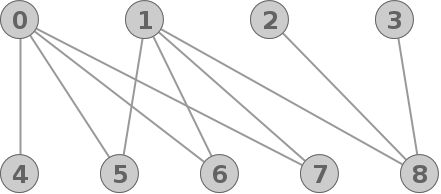
\includegraphics[scale = 0.2]{img/ej3/busqueda_local/k5,4Nocompleto_st0.png} &
			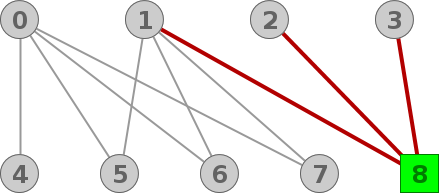
\includegraphics[scale = 0.2]{img/ej3/busqueda_local/k5,4Nocompleto_st1.png} & 
			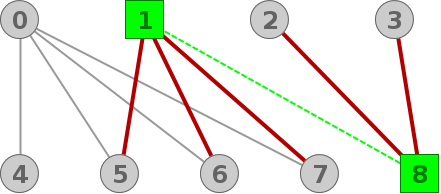
\includegraphics[scale = 0.2]{img/ej3/busqueda_local/k5,4Nocompleto_st2.png} \\
		\hline
		\end{tabular}
	\end{center}
\end{figure}
En este caso el grado promedio es $2,2$ con lo que podr\'ia suceder 
(con las etiquetas correctas) que la busqueda local comience con el
nodo marcado como $8$ en el ejemplo, cosa que en la golosa 
constructiva no pod\'ia suceder.

Para los \'arboles tambi\'en analizaremos el caso extremo presentado 
en la figura \ref{fig:extremo_arboles} y analizaremos nuevamente
la curiosidad de que debido a la relajaci\'on en el criterio de 
selecci\'on del primer nodo en busqueda local, existe una 
construccion alternativa de la clique devuelta por la heur\'istica
aunque sobre este ejemplo la respuesta ser\'a sub-optima.

\begin{figure}[H]
\caption{Resultado sub-\'optimo del ejemplo extremo para \'arboles - 
Forma alternativa}
\begin{center}
		\begin{tabular}{|c||c||c|}
		\hline
		Grafo de entrada & Paso 1 & Paso 2 \\ 
			\hline
			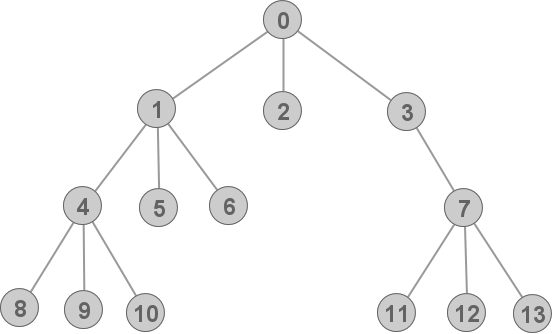
\includegraphics[scale = 0.2]{img/ej3/busqueda_local/extremetree_st0.png} &
			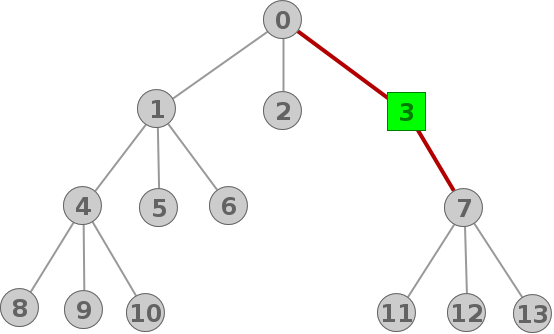
\includegraphics[scale = 0.2]{img/ej3/busqueda_local/extremetree_st11.png} & 
			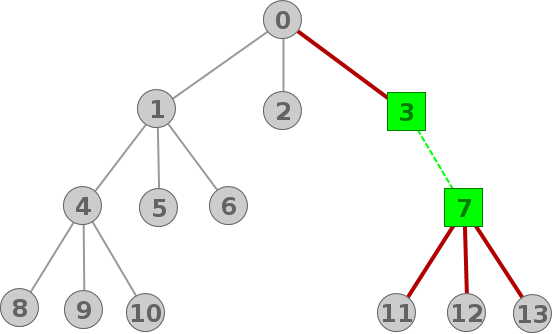
\includegraphics[scale = 0.2]{img/ej3/busqueda_local/extremetree_st12.png} \\
		\hline
		\end{tabular}
	\end{center}
\end{figure}
Notar que aqu\'i el grado promedio es aproximadamente $1,8$ con lo que 
el nodo identificado como $3$ en el ejemplo es elegible como
primer nodo de $K$ pues $2 > 1,8$.

\subsubsection{Estrella + Puente + CMF}

En esta familia, siguiendo con la idea de las \'ultimas dos analizadas
podemos ver que que para llegar a la soluci\'on \'optima hay muchos 
m\'as puntos de inicio que en la golosa constructiva. Por ejemplo
el primer nodo puede estar en $K_{\Delta -1}$ y no ser siquiera $v'$ 
(ver Figura \ref{fig:epcmf_carac}), en los casos en los que esto 
suceda, en la variante b\'asica, la busqueda local elegir\'a
$\left\lfloor \frac{\Delta -1}{2} \right\rfloor$ nodos de $K_{\Delta -1}$. 
Si estos nodos incluyen a $v'$, termina pues no quedan candidatos que
hagan crecer la soluci\'on parcial, si no lo incluyen hay dos posibilidades:

\begin{itemize}
	\item $\Delta$ par: La cantidad de nodos en $K_{\Delta -1}$ ser\'a impar 
	y entonces la soluci\'on crece hasta alcanzar
	$\left\lfloor \frac{\Delta -1}{2} \right\rfloor$ nodos que por hip\'otesis
	no incluyen a $v'$, en el siguiente paso el \'unico candidato restante
	que hace crecer la soluci\'on en una arista es $v'$ y por ello lo agrega 
	a la soluci\'on, terminando con una soluci\'on \'optima.
	\begin{center}
	\begin{tabular}{|c||c|}
		\hline
		Grafo entrada & 
		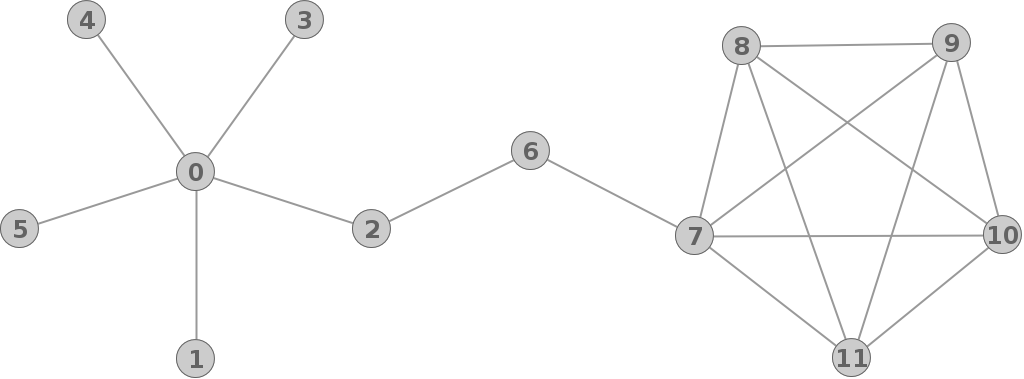
\includegraphics[scale = 0.2]{img/ej3/busqueda_local/estrellaPuenteCMFImpar.png} \\
		\hline
		Primer paso &
		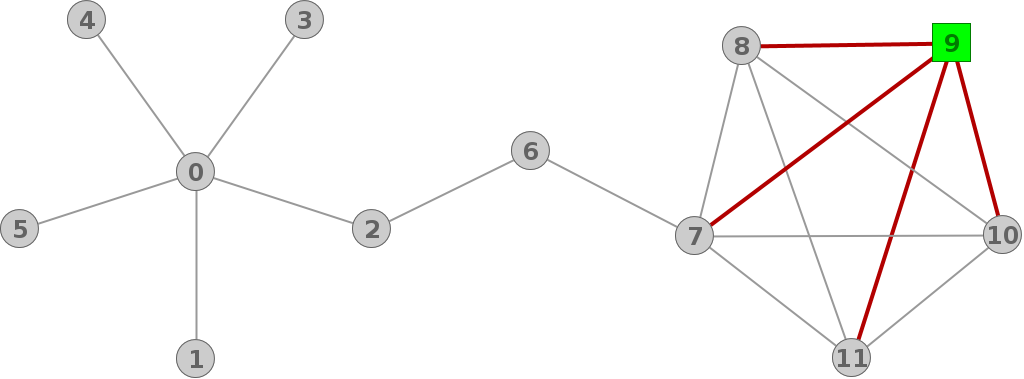
\includegraphics[scale = 0.2]{img/ej3/busqueda_local/estrellaPuenteCMFImpar_st01.png} \\
		\hline
		Segundo paso &
		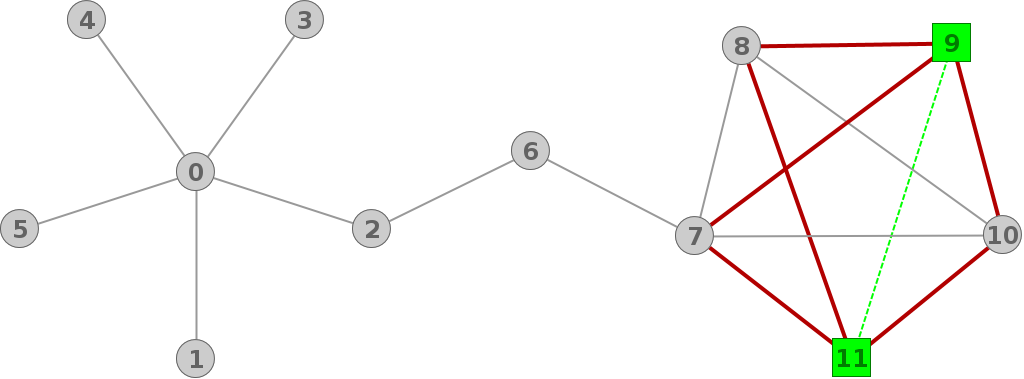
\includegraphics[scale = 0.2]{img/ej3/busqueda_local/estrellaPuenteCMFImpar_st02.png} \\
		\hline
		Tercer paso &
		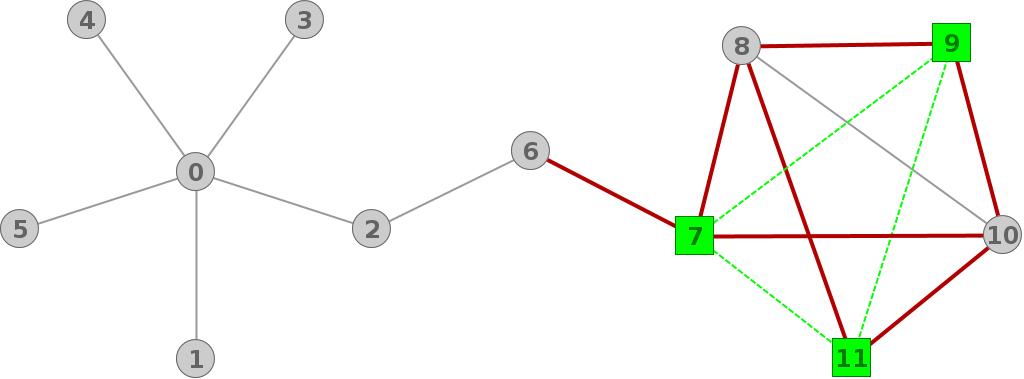
\includegraphics[scale = 0.2]{img/ej3/busqueda_local/estrellaPuenteCMFImpar_st03.png} \\
		\hline

	\end{tabular}
	\end{center}


	\item $\Delta$ impar: La cantidad de nodos en $K_{\Delta -1}$ ser\'a par, 
	en este caso la soluci\'on crece hasta alcanzar $\frac{\Delta -1}{2}$ nodos
	que no incluyen a $v'$, llegados a este punto la soluci\'on no puede crecer
	para incluir a $v'$ ya que de hacerlo la frontera de la soluci\'on ser\'ia
	la misma que en el paso anterior y el algoritmo no se comporta de esta manera.
	Por ende la soluci\'on devuelta es sub-\'optima.
	\begin{center}
	\begin{tabular}{|c||c|}
		\hline
		Grafo entrada & 
		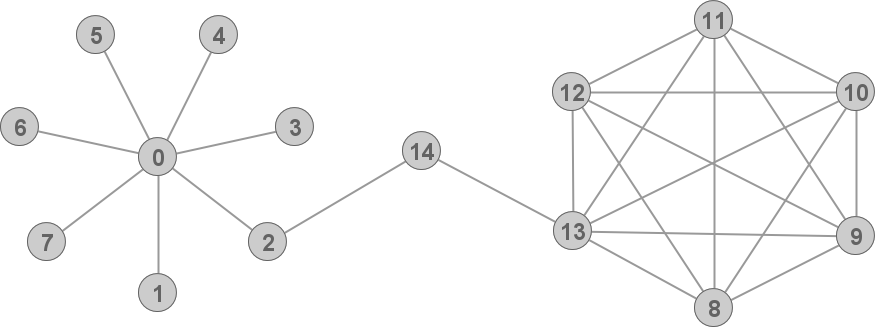
\includegraphics[scale = 0.2]{img/ej3/busqueda_local/estrellaPuenteCMFPar.png} \\
		\hline
		Primer paso &
		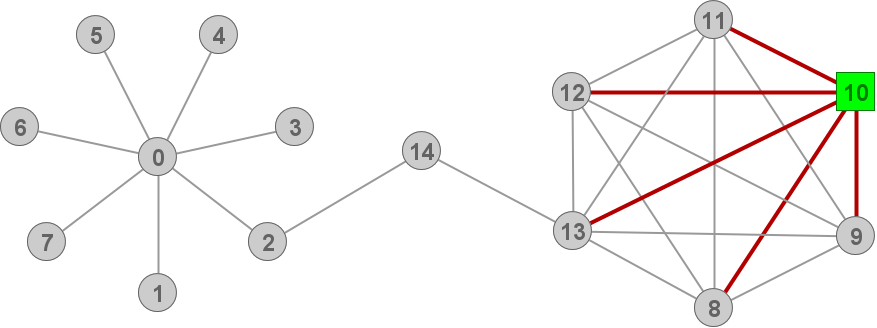
\includegraphics[scale = 0.2]{img/ej3/busqueda_local/estrellaPuenteCMFPar_st01.png} \\
		\hline
		Segundo paso &
		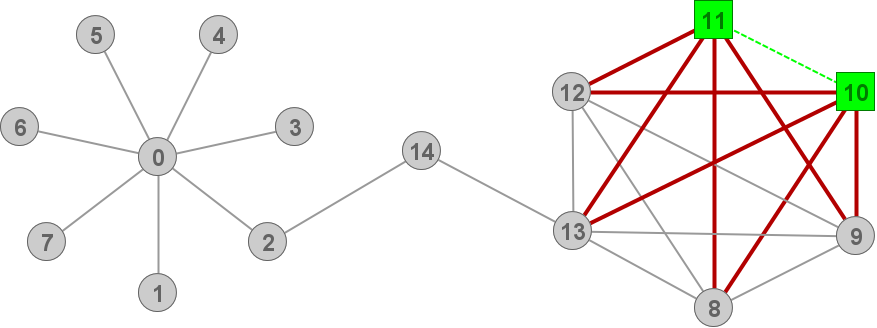
\includegraphics[scale = 0.2]{img/ej3/busqueda_local/estrellaPuenteCMFPar_st02.png} \\
		\hline
		Tercer paso &
		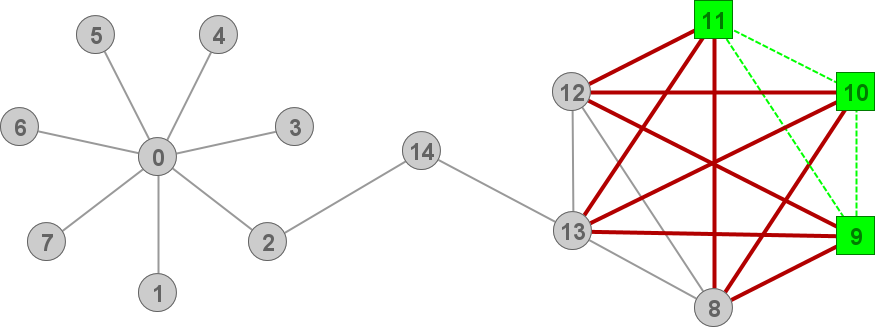
\includegraphics[scale = 0.2]{img/ej3/busqueda_local/estrellaPuenteCMFPar_st03.png} \\
		\hline

	\end{tabular}
	\end{center}


\end{itemize}

Notar que en la variante \emph{Mejor Vecino} evita el resultado sub-\'optimo en 
el \'ultimo caso (bajo las hip\'otesis del mismo).

Hay otros posibles comportamientos de la heur\'istica sobre la misma familia de
grafos, que el algoritmo comience la soluci\'on en uno de los nodos del puente o
que la comience en el centro de la estrella.

Que comience la soluci\'on sobre el puente es un caso que t\'ipicamente no va a 
suceder, si es un puente simple (camino simple) la \'unica forma de que sucediera
ser\'ia si el puente es lo suficientemente largo para bajar el grado promedio a
un valor menor a dos, si el puente no es un camino simple y en cambio tiene nodos
extra, el puente no tendr\'a que ser tan largo pero siempre se deber\'a cumplir
que el nodo inicial de la soluci\'on tenga grado mayor al grado promedio del grafo.

Cuando la soluci\'on se inicia en el centro de la estrella, la busqueda local 
se estanca en el m\'aximo local debido al puente que une la estrella con $K_{\Delta -1}$,
de hecho, esta familia fue dise\~nada con el objetivo de asegurar precisamente
este estancamiento.
		



\subsection{Experimentaci\'on}
    \subsubsection{Resultados}
\par Se presentan a continuaci\'on los resultados de la experimentaci\'on
    de la heur\'istica golosa constructiva para \emph{CMF}. La experimentaci\'on se realiz\'o
    con las instancias ya generadas (seg\'un se explica en \emph{\nameref{notas_preliminares},
    \nameref{notas:datasets}} y \emph{\nameref{notas:experimentacion}}).

\par Para recordar, se cuentan con 10 instancias aleatorias de cada tama\~no,
    las cuales fueron resueltas 5 veces cada una y nos quedamos con el menor tiempo
    requerido de esas 5 ejecuciones. Por \'ultimo, tomamos el promedio de este tiempo
    requerido calculado entre las instancias del mismo tama\~no (10, como se ha
    dicho).

\bigskip

\begin{figure}[H]
    \centering
    \fontsize{8}{10}\selectfont
    \resizebox{0.8\textwidth}{!}{% GNUPLOT: LaTeX picture with Postscript
\begingroup
  \makeatletter
  \providecommand\color[2][]{%
    \GenericError{(gnuplot) \space\space\space\@spaces}{%
      Package color not loaded in conjunction with
      terminal option `colourtext'%
    }{See the gnuplot documentation for explanation.%
    }{Either use 'blacktext' in gnuplot or load the package
      color.sty in LaTeX.}%
    \renewcommand\color[2][]{}%
  }%
  \providecommand\includegraphics[2][]{%
    \GenericError{(gnuplot) \space\space\space\@spaces}{%
      Package graphicx or graphics not loaded%
    }{See the gnuplot documentation for explanation.%
    }{The gnuplot epslatex terminal needs graphicx.sty or graphics.sty.}%
    \renewcommand\includegraphics[2][]{}%
  }%
  \providecommand\rotatebox[2]{#2}%
  \@ifundefined{ifGPcolor}{%
    \newif\ifGPcolor
    \GPcolortrue
  }{}%
  \@ifundefined{ifGPblacktext}{%
    \newif\ifGPblacktext
    \GPblacktexttrue
  }{}%
  % define a \g@addto@macro without @ in the name:
  \let\gplgaddtomacro\g@addto@macro
  % define empty templates for all commands taking text:
  \gdef\gplbacktext{}%
  \gdef\gplfronttext{}%
  \makeatother
  \ifGPblacktext
    % no textcolor at all
    \def\colorrgb#1{}%
    \def\colorgray#1{}%
  \else
    % gray or color?
    \ifGPcolor
      \def\colorrgb#1{\color[rgb]{#1}}%
      \def\colorgray#1{\color[gray]{#1}}%
      \expandafter\def\csname LTw\endcsname{\color{white}}%
      \expandafter\def\csname LTb\endcsname{\color{black}}%
      \expandafter\def\csname LTa\endcsname{\color{black}}%
      \expandafter\def\csname LT0\endcsname{\color[rgb]{1,0,0}}%
      \expandafter\def\csname LT1\endcsname{\color[rgb]{0,1,0}}%
      \expandafter\def\csname LT2\endcsname{\color[rgb]{0,0,1}}%
      \expandafter\def\csname LT3\endcsname{\color[rgb]{1,0,1}}%
      \expandafter\def\csname LT4\endcsname{\color[rgb]{0,1,1}}%
      \expandafter\def\csname LT5\endcsname{\color[rgb]{1,1,0}}%
      \expandafter\def\csname LT6\endcsname{\color[rgb]{0,0,0}}%
      \expandafter\def\csname LT7\endcsname{\color[rgb]{1,0.3,0}}%
      \expandafter\def\csname LT8\endcsname{\color[rgb]{0.5,0.5,0.5}}%
    \else
      % gray
      \def\colorrgb#1{\color{black}}%
      \def\colorgray#1{\color[gray]{#1}}%
      \expandafter\def\csname LTw\endcsname{\color{white}}%
      \expandafter\def\csname LTb\endcsname{\color{black}}%
      \expandafter\def\csname LTa\endcsname{\color{black}}%
      \expandafter\def\csname LT0\endcsname{\color{black}}%
      \expandafter\def\csname LT1\endcsname{\color{black}}%
      \expandafter\def\csname LT2\endcsname{\color{black}}%
      \expandafter\def\csname LT3\endcsname{\color{black}}%
      \expandafter\def\csname LT4\endcsname{\color{black}}%
      \expandafter\def\csname LT5\endcsname{\color{black}}%
      \expandafter\def\csname LT6\endcsname{\color{black}}%
      \expandafter\def\csname LT7\endcsname{\color{black}}%
      \expandafter\def\csname LT8\endcsname{\color{black}}%
    \fi
  \fi
  \setlength{\unitlength}{0.0500bp}%
  \begin{picture}(7200.00,5040.00)%
    \gplgaddtomacro\gplbacktext{%
      \csname LTb\endcsname%
      \put(1430,2244){\makebox(0,0)[r]{\strut{} 0}}%
      \csname LTb\endcsname%
      \put(1430,2549){\makebox(0,0)[r]{\strut{} 5000}}%
      \csname LTb\endcsname%
      \put(1430,2854){\makebox(0,0)[r]{\strut{} 10000}}%
      \csname LTb\endcsname%
      \put(1430,3159){\makebox(0,0)[r]{\strut{} 15000}}%
      \csname LTb\endcsname%
      \put(1430,3464){\makebox(0,0)[r]{\strut{} 20000}}%
      \csname LTb\endcsname%
      \put(1430,3769){\makebox(0,0)[r]{\strut{} 25000}}%
      \csname LTb\endcsname%
      \put(1430,4074){\makebox(0,0)[r]{\strut{} 30000}}%
      \csname LTb\endcsname%
      \put(1430,4379){\makebox(0,0)[r]{\strut{} 35000}}%
      \csname LTb\endcsname%
      \put(1562,2024){\makebox(0,0){\strut{} 0}}%
      \csname LTb\endcsname%
      \put(2086,2024){\makebox(0,0){\strut{} 500}}%
      \csname LTb\endcsname%
      \put(2610,2024){\makebox(0,0){\strut{} 1000}}%
      \csname LTb\endcsname%
      \put(3134,2024){\makebox(0,0){\strut{} 1500}}%
      \csname LTb\endcsname%
      \put(3658,2024){\makebox(0,0){\strut{} 2000}}%
      \csname LTb\endcsname%
      \put(4183,2024){\makebox(0,0){\strut{} 2500}}%
      \csname LTb\endcsname%
      \put(4707,2024){\makebox(0,0){\strut{} 3000}}%
      \csname LTb\endcsname%
      \put(5231,2024){\makebox(0,0){\strut{} 3500}}%
      \csname LTb\endcsname%
      \put(5755,2024){\makebox(0,0){\strut{} 4000}}%
      \csname LTb\endcsname%
      \put(6279,2024){\makebox(0,0){\strut{} 4500}}%
      \csname LTb\endcsname%
      \put(6803,2024){\makebox(0,0){\strut{} 5000}}%
      \put(176,3311){\rotatebox{-270}{\makebox(0,0){\strut{}Tiempo (nanosegundos)}}}%
      \put(396,3311){\rotatebox{-270}{\makebox(0,0){\strut{}(Escala Lineal)}}}%
      \put(4182,1694){\makebox(0,0){\strut{}Cantidad de Nodos}}%
      \put(4182,1474){\makebox(0,0){\strut{}(Escala Lineal)}}%
      \put(4182,4709){\makebox(0,0){\strut{}Tiempo de ejecución conforme aumenta la cantidad de nodos}}%
    }%
    \gplgaddtomacro\gplfronttext{%
      \csname LTb\endcsname%
      \put(5735,1053){\makebox(0,0)[r]{\strut{}Grafos Completos}}%
      \csname LTb\endcsname%
      \put(5735,833){\makebox(0,0)[r]{\strut{}Arboles}}%
      \csname LTb\endcsname%
      \put(5735,613){\makebox(0,0)[r]{\strut{}Circulares}}%
      \csname LTb\endcsname%
      \put(5735,393){\makebox(0,0)[r]{\strut{}Cota teórica superior $\mathcal O(n^2)$}}%
      \csname LTb\endcsname%
      \put(5735,173){\makebox(0,0)[r]{\strut{}Cota teórica superior $\mathcal O(n)$}}%
    }%
    \gplbacktext
    \put(0,0){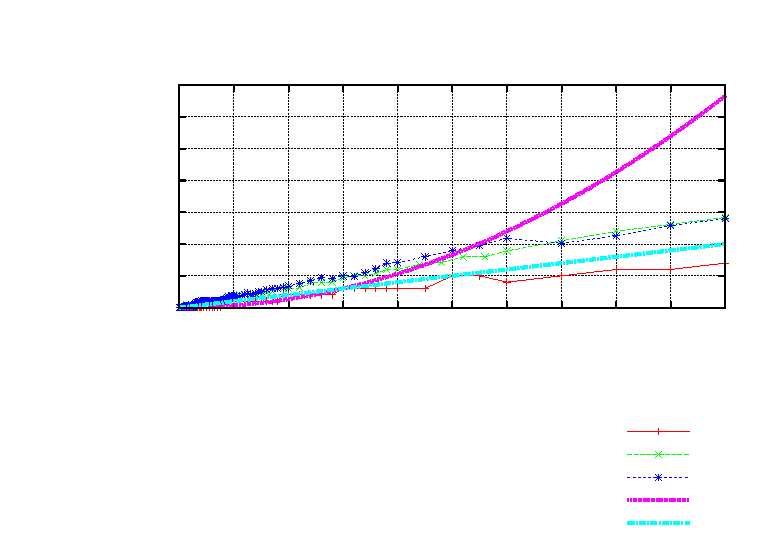
\includegraphics{ej3_nodos_completos_arboles_circulares}}%
    \gplfronttext
  \end{picture}%
\endgroup
}
    \caption{Complejidad temporal para grafos completos, \'arboles y circulares}
\end{figure}

\begin{figure}[H]
    \centering
    \fontsize{8}{10}\selectfont
    \resizebox{0.8\textwidth}{!}{% GNUPLOT: LaTeX picture with Postscript
\begingroup
  \makeatletter
  \providecommand\color[2][]{%
    \GenericError{(gnuplot) \space\space\space\@spaces}{%
      Package color not loaded in conjunction with
      terminal option `colourtext'%
    }{See the gnuplot documentation for explanation.%
    }{Either use 'blacktext' in gnuplot or load the package
      color.sty in LaTeX.}%
    \renewcommand\color[2][]{}%
  }%
  \providecommand\includegraphics[2][]{%
    \GenericError{(gnuplot) \space\space\space\@spaces}{%
      Package graphicx or graphics not loaded%
    }{See the gnuplot documentation for explanation.%
    }{The gnuplot epslatex terminal needs graphicx.sty or graphics.sty.}%
    \renewcommand\includegraphics[2][]{}%
  }%
  \providecommand\rotatebox[2]{#2}%
  \@ifundefined{ifGPcolor}{%
    \newif\ifGPcolor
    \GPcolortrue
  }{}%
  \@ifundefined{ifGPblacktext}{%
    \newif\ifGPblacktext
    \GPblacktexttrue
  }{}%
  % define a \g@addto@macro without @ in the name:
  \let\gplgaddtomacro\g@addto@macro
  % define empty templates for all commands taking text:
  \gdef\gplbacktext{}%
  \gdef\gplfronttext{}%
  \makeatother
  \ifGPblacktext
    % no textcolor at all
    \def\colorrgb#1{}%
    \def\colorgray#1{}%
  \else
    % gray or color?
    \ifGPcolor
      \def\colorrgb#1{\color[rgb]{#1}}%
      \def\colorgray#1{\color[gray]{#1}}%
      \expandafter\def\csname LTw\endcsname{\color{white}}%
      \expandafter\def\csname LTb\endcsname{\color{black}}%
      \expandafter\def\csname LTa\endcsname{\color{black}}%
      \expandafter\def\csname LT0\endcsname{\color[rgb]{1,0,0}}%
      \expandafter\def\csname LT1\endcsname{\color[rgb]{0,1,0}}%
      \expandafter\def\csname LT2\endcsname{\color[rgb]{0,0,1}}%
      \expandafter\def\csname LT3\endcsname{\color[rgb]{1,0,1}}%
      \expandafter\def\csname LT4\endcsname{\color[rgb]{0,1,1}}%
      \expandafter\def\csname LT5\endcsname{\color[rgb]{1,1,0}}%
      \expandafter\def\csname LT6\endcsname{\color[rgb]{0,0,0}}%
      \expandafter\def\csname LT7\endcsname{\color[rgb]{1,0.3,0}}%
      \expandafter\def\csname LT8\endcsname{\color[rgb]{0.5,0.5,0.5}}%
    \else
      % gray
      \def\colorrgb#1{\color{black}}%
      \def\colorgray#1{\color[gray]{#1}}%
      \expandafter\def\csname LTw\endcsname{\color{white}}%
      \expandafter\def\csname LTb\endcsname{\color{black}}%
      \expandafter\def\csname LTa\endcsname{\color{black}}%
      \expandafter\def\csname LT0\endcsname{\color{black}}%
      \expandafter\def\csname LT1\endcsname{\color{black}}%
      \expandafter\def\csname LT2\endcsname{\color{black}}%
      \expandafter\def\csname LT3\endcsname{\color{black}}%
      \expandafter\def\csname LT4\endcsname{\color{black}}%
      \expandafter\def\csname LT5\endcsname{\color{black}}%
      \expandafter\def\csname LT6\endcsname{\color{black}}%
      \expandafter\def\csname LT7\endcsname{\color{black}}%
      \expandafter\def\csname LT8\endcsname{\color{black}}%
    \fi
  \fi
  \setlength{\unitlength}{0.0500bp}%
  \begin{picture}(7200.00,5040.00)%
    \gplgaddtomacro\gplbacktext{%
      \csname LTb\endcsname%
      \put(1166,2244){\makebox(0,0)[r]{\strut{} 0}}%
      \csname LTb\endcsname%
      \put(1166,2511){\makebox(0,0)[r]{\strut{} 100}}%
      \csname LTb\endcsname%
      \put(1166,2778){\makebox(0,0)[r]{\strut{} 200}}%
      \csname LTb\endcsname%
      \put(1166,3045){\makebox(0,0)[r]{\strut{} 300}}%
      \csname LTb\endcsname%
      \put(1166,3312){\makebox(0,0)[r]{\strut{} 400}}%
      \csname LTb\endcsname%
      \put(1166,3578){\makebox(0,0)[r]{\strut{} 500}}%
      \csname LTb\endcsname%
      \put(1166,3845){\makebox(0,0)[r]{\strut{} 600}}%
      \csname LTb\endcsname%
      \put(1166,4112){\makebox(0,0)[r]{\strut{} 700}}%
      \csname LTb\endcsname%
      \put(1166,4379){\makebox(0,0)[r]{\strut{} 800}}%
      \csname LTb\endcsname%
      \put(1298,2024){\makebox(0,0){\strut{} 0}}%
      \csname LTb\endcsname%
      \put(1849,2024){\makebox(0,0){\strut{} 500}}%
      \csname LTb\endcsname%
      \put(2399,2024){\makebox(0,0){\strut{} 1000}}%
      \csname LTb\endcsname%
      \put(2950,2024){\makebox(0,0){\strut{} 1500}}%
      \csname LTb\endcsname%
      \put(3500,2024){\makebox(0,0){\strut{} 2000}}%
      \csname LTb\endcsname%
      \put(4051,2024){\makebox(0,0){\strut{} 2500}}%
      \csname LTb\endcsname%
      \put(4601,2024){\makebox(0,0){\strut{} 3000}}%
      \csname LTb\endcsname%
      \put(5152,2024){\makebox(0,0){\strut{} 3500}}%
      \csname LTb\endcsname%
      \put(5702,2024){\makebox(0,0){\strut{} 4000}}%
      \csname LTb\endcsname%
      \put(6253,2024){\makebox(0,0){\strut{} 4500}}%
      \csname LTb\endcsname%
      \put(6803,2024){\makebox(0,0){\strut{} 5000}}%
      \put(176,3311){\rotatebox{-270}{\makebox(0,0){\strut{}Tiempo (microsegundos)}}}%
      \put(396,3311){\rotatebox{-270}{\makebox(0,0){\strut{}(Escala Lineal)}}}%
      \put(4050,1694){\makebox(0,0){\strut{}Cantidad de Nodos}}%
      \put(4050,1474){\makebox(0,0){\strut{}(Escala Lineal)}}%
      \put(4050,4709){\makebox(0,0){\strut{}Tiempo de ejecución conforme aumenta la cantidad de nodos}}%
    }%
    \gplgaddtomacro\gplfronttext{%
      \csname LTb\endcsname%
      \put(5603,1053){\makebox(0,0)[r]{\strut{}Estrellas}}%
      \csname LTb\endcsname%
      \put(5603,833){\makebox(0,0)[r]{\strut{}Ruedas}}%
      \csname LTb\endcsname%
      \put(5603,613){\makebox(0,0)[r]{\strut{}Banana Tree}}%
      \csname LTb\endcsname%
      \put(5603,393){\makebox(0,0)[r]{\strut{}Bipartitos}}%
      \csname LTb\endcsname%
      \put(5603,173){\makebox(0,0)[r]{\strut{}Cota teórica superior $\mathcal O(n^2)$}}%
    }%
    \gplbacktext
    \put(0,0){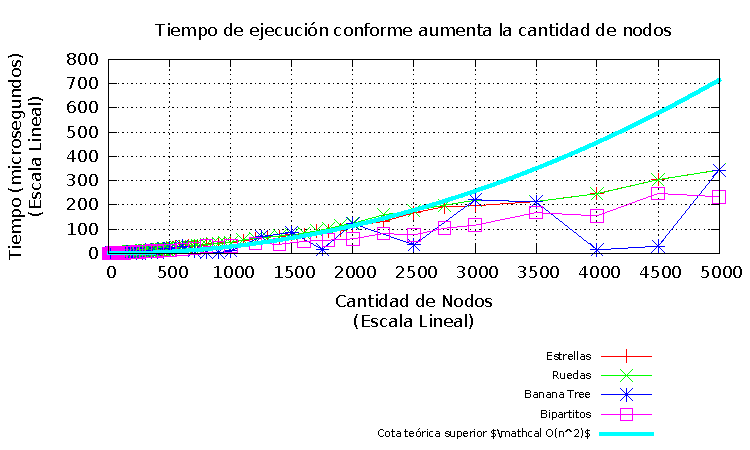
\includegraphics{ej3_nodos_estrella_rueda_banana_bipartito}}%
    \gplfronttext
  \end{picture}%
\endgroup
}
    \caption{Complejidad temporal para grafos estrella, rueda, banana tree y bipartitos}
\end{figure}

\begin{figure}[H]
    \centering
    \fontsize{8}{10}\selectfont
    \resizebox{0.8\textwidth}{!}{% GNUPLOT: LaTeX picture with Postscript
\begingroup
  \makeatletter
  \providecommand\color[2][]{%
    \GenericError{(gnuplot) \space\space\space\@spaces}{%
      Package color not loaded in conjunction with
      terminal option `colourtext'%
    }{See the gnuplot documentation for explanation.%
    }{Either use 'blacktext' in gnuplot or load the package
      color.sty in LaTeX.}%
    \renewcommand\color[2][]{}%
  }%
  \providecommand\includegraphics[2][]{%
    \GenericError{(gnuplot) \space\space\space\@spaces}{%
      Package graphicx or graphics not loaded%
    }{See the gnuplot documentation for explanation.%
    }{The gnuplot epslatex terminal needs graphicx.sty or graphics.sty.}%
    \renewcommand\includegraphics[2][]{}%
  }%
  \providecommand\rotatebox[2]{#2}%
  \@ifundefined{ifGPcolor}{%
    \newif\ifGPcolor
    \GPcolortrue
  }{}%
  \@ifundefined{ifGPblacktext}{%
    \newif\ifGPblacktext
    \GPblacktexttrue
  }{}%
  % define a \g@addto@macro without @ in the name:
  \let\gplgaddtomacro\g@addto@macro
  % define empty templates for all commands taking text:
  \gdef\gplbacktext{}%
  \gdef\gplfronttext{}%
  \makeatother
  \ifGPblacktext
    % no textcolor at all
    \def\colorrgb#1{}%
    \def\colorgray#1{}%
  \else
    % gray or color?
    \ifGPcolor
      \def\colorrgb#1{\color[rgb]{#1}}%
      \def\colorgray#1{\color[gray]{#1}}%
      \expandafter\def\csname LTw\endcsname{\color{white}}%
      \expandafter\def\csname LTb\endcsname{\color{black}}%
      \expandafter\def\csname LTa\endcsname{\color{black}}%
      \expandafter\def\csname LT0\endcsname{\color[rgb]{1,0,0}}%
      \expandafter\def\csname LT1\endcsname{\color[rgb]{0,1,0}}%
      \expandafter\def\csname LT2\endcsname{\color[rgb]{0,0,1}}%
      \expandafter\def\csname LT3\endcsname{\color[rgb]{1,0,1}}%
      \expandafter\def\csname LT4\endcsname{\color[rgb]{0,1,1}}%
      \expandafter\def\csname LT5\endcsname{\color[rgb]{1,1,0}}%
      \expandafter\def\csname LT6\endcsname{\color[rgb]{0,0,0}}%
      \expandafter\def\csname LT7\endcsname{\color[rgb]{1,0.3,0}}%
      \expandafter\def\csname LT8\endcsname{\color[rgb]{0.5,0.5,0.5}}%
    \else
      % gray
      \def\colorrgb#1{\color{black}}%
      \def\colorgray#1{\color[gray]{#1}}%
      \expandafter\def\csname LTw\endcsname{\color{white}}%
      \expandafter\def\csname LTb\endcsname{\color{black}}%
      \expandafter\def\csname LTa\endcsname{\color{black}}%
      \expandafter\def\csname LT0\endcsname{\color{black}}%
      \expandafter\def\csname LT1\endcsname{\color{black}}%
      \expandafter\def\csname LT2\endcsname{\color{black}}%
      \expandafter\def\csname LT3\endcsname{\color{black}}%
      \expandafter\def\csname LT4\endcsname{\color{black}}%
      \expandafter\def\csname LT5\endcsname{\color{black}}%
      \expandafter\def\csname LT6\endcsname{\color{black}}%
      \expandafter\def\csname LT7\endcsname{\color{black}}%
      \expandafter\def\csname LT8\endcsname{\color{black}}%
    \fi
  \fi
  \setlength{\unitlength}{0.0500bp}%
  \begin{picture}(7200.00,5040.00)%
    \gplgaddtomacro\gplbacktext{%
      \csname LTb\endcsname%
      \put(1166,1804){\makebox(0,0)[r]{\strut{} 0}}%
      \csname LTb\endcsname%
      \put(1166,2090){\makebox(0,0)[r]{\strut{} 50}}%
      \csname LTb\endcsname%
      \put(1166,2376){\makebox(0,0)[r]{\strut{} 100}}%
      \csname LTb\endcsname%
      \put(1166,2662){\makebox(0,0)[r]{\strut{} 150}}%
      \csname LTb\endcsname%
      \put(1166,2948){\makebox(0,0)[r]{\strut{} 200}}%
      \csname LTb\endcsname%
      \put(1166,3235){\makebox(0,0)[r]{\strut{} 250}}%
      \csname LTb\endcsname%
      \put(1166,3521){\makebox(0,0)[r]{\strut{} 300}}%
      \csname LTb\endcsname%
      \put(1166,3807){\makebox(0,0)[r]{\strut{} 350}}%
      \csname LTb\endcsname%
      \put(1166,4093){\makebox(0,0)[r]{\strut{} 400}}%
      \csname LTb\endcsname%
      \put(1166,4379){\makebox(0,0)[r]{\strut{} 450}}%
      \csname LTb\endcsname%
      \put(1298,1584){\makebox(0,0){\strut{} 0}}%
      \csname LTb\endcsname%
      \put(1849,1584){\makebox(0,0){\strut{} 500}}%
      \csname LTb\endcsname%
      \put(2399,1584){\makebox(0,0){\strut{} 1000}}%
      \csname LTb\endcsname%
      \put(2950,1584){\makebox(0,0){\strut{} 1500}}%
      \csname LTb\endcsname%
      \put(3500,1584){\makebox(0,0){\strut{} 2000}}%
      \csname LTb\endcsname%
      \put(4051,1584){\makebox(0,0){\strut{} 2500}}%
      \csname LTb\endcsname%
      \put(4601,1584){\makebox(0,0){\strut{} 3000}}%
      \csname LTb\endcsname%
      \put(5152,1584){\makebox(0,0){\strut{} 3500}}%
      \csname LTb\endcsname%
      \put(5702,1584){\makebox(0,0){\strut{} 4000}}%
      \csname LTb\endcsname%
      \put(6253,1584){\makebox(0,0){\strut{} 4500}}%
      \csname LTb\endcsname%
      \put(6803,1584){\makebox(0,0){\strut{} 5000}}%
      \put(176,3091){\rotatebox{-270}{\makebox(0,0){\strut{}Tiempo (microsegundos)}}}%
      \put(396,3091){\rotatebox{-270}{\makebox(0,0){\strut{}(Escala Lineal)}}}%
      \put(4050,1254){\makebox(0,0){\strut{}Cantidad de Nodos}}%
      \put(4050,1034){\makebox(0,0){\strut{}(Escala Lineal)}}%
      \put(4050,4709){\makebox(0,0){\strut{}Tiempo de ejecución conforme aumenta la cantidad de nodos}}%
    }%
    \gplgaddtomacro\gplfronttext{%
      \csname LTb\endcsname%
      \put(5603,613){\makebox(0,0)[r]{\strut{}Estrella+CMF}}%
      \csname LTb\endcsname%
      \put(5603,393){\makebox(0,0)[r]{\strut{}Estrella+Puente+CMF}}%
      \csname LTb\endcsname%
      \put(5603,173){\makebox(0,0)[r]{\strut{}Cota teórica superior $\mathcal O(n^2)$}}%
    }%
    \gplbacktext
    \put(0,0){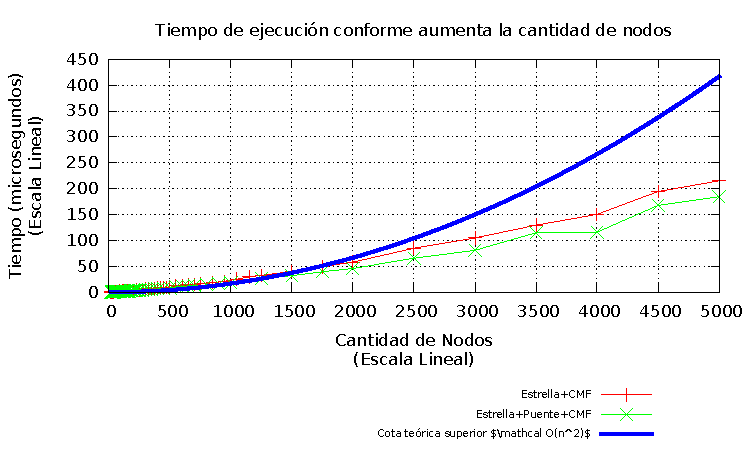
\includegraphics{ej3_nodos_disruptivas}}%
    \gplfronttext
  \end{picture}%
\endgroup
}
    \caption{Complejidad temporal para grafos Estrella+CMF, Estrella+Puente+CMF}
\end{figure}

\subsubsection{Conclusiones}
\par En los primeros 2 resultados se puede observar que la complejidad asint\'otica
    para las familias ``simples''\footnote{Consideramos a los grafos completos
    como una familia simple pues con los datos de entrada resolver el problema
    de \emph{CMF} es trivial.} (pocas aristas y con estructuras muy restrictivas)
    es similar. Si bien hay diferencias (en el orden de los nanosegundos), se
    destaca que todas cumplen con la complejidad asint\'otica temporal te\'orica
    calculada y a su vez se comportan de la misma manera en cuanto a crecimiento.

\par En el segundo gr\'afico, tambi\'en se cuentan con una serie de familias
    ``simples'', pero aqu\'i el comportamiento de nuestra heur\'istica resulta
    un tanto m\'as err\'atico, si bien sigue estando en el orden de complejidad
    calculado. Se puede observar que mientras que las familias de las 
    Rueadas y las estrellas (de estructuras muy similares) se comportan pr\'acticamente
    igual, para los grafos bipartitos se requiere menor tiempo para resolver
    instancias del mismo tama\~no. Esto es un tanto raro, ya que en las 3 familias
    (como ya se ha explicado) la \emph{CMF} tendr\'a el mismo tama\~no. S\'olo
    nos queda hipotetizar\footnote{Viernes 22 de Noviembre, 17:58 hs GMT-3} sobre los motivos.

\par En el caso de la familia de grafos \emph{Banana Tree}, suponemos que su comportamiento
    se debe que seg\'un el tama\~no de las estrellas que tenga en sus extremos, el nodo
    de mayor grado estar\'a en alguna estrella o en el nodo central que une a todas las estrellas.
    Este dato tendr\'a una influencia inmediata en la elecci\'on de los nodos candidatos
    a agregarse a la clique luego de haber encontrado el nodo de mayor grado del grafo (ya
    que si las estrellas/extremidades son de tama\~no considerable, las mismas
    deberan ser tenidas en cuenta, mientras que si solo se tiene una gran estrella (las
    ``bananas'' son de taman\~o 1), esto ser\'a m\'as eficiente.

\par Por \'ultimo, observamos que el comportamiento para las familias Estrella+CMF y
    Estrella+Puente+CMF es muy estable a medida que crece el taman\~o de las instancias.
    Quiz\'as lo m\'as interesantes de estas familias (aparte de comprobar que cumplen
    con la complejidad asint\'otica te\'orica) es comparar los resultados otorgados
    por la heur\'istica con el algoritmo exacto u las dem\'as heur\'isticas. Esto
    se efectua en la Secci\'on~\ref{experimentacion} de este trabajo.


        \pagebreak

    \section{Heur\'istica Constructiva Golosa}
        \subsection{Resoluci\'on}
    \begin{algorithm}[H]
    \caption{Heur\'istica Golosa Constructiva 1 para \emph{CMF} - Descriptivo}
    \begin{algorithmic}[1]
        \Require\Statex
            \begin{itemize}
                \item Un grafo $G$ de $n$ v\'ertices y $m$ aristas.

                \item Una funci\'on $candidatos(K)$, que dado un conjunto de v\'ertices
                    $K$, devuelve el conjunto de v\'ertices de $G$ que son adjacentes
                    a todos los elementos de $K$, cuyo grado es mayor $2|K|$.
            \end{itemize}

        \Statex

        \Ensure Una \emph{clique} $K$ de $G$ con una frontera $\delta(K)$ que se
            espera que sea de cardinalidad cercana o igual a la de $\delta(K')$,
            siendo $K'$ la \emph{clique} de m\'axima frontera de $G$.

        \Statex

        \State Sea $v$ el v\'ertice de mayor grado en $G$.
        \State $K \gets \{v\}$
        \While{$candidatos(K) \neq \emptyset$}
            \State Sea $v'$ el v\'ertice de mayor grado en $candidatos(K)$.
            \State $K \gets K \cup \{v'\}$
        \EndWhile

        \State \Return{$K$}
    \end{algorithmic}
\end{algorithm}

\begin{algorithm}[H]
    \caption{Heur\'istica Golosa Constructiva 2 para \emph{CMF} - Descriptivo}
    \begin{algorithmic}[1]
        \Require Un grafo $G$ de $n$ v\'ertices y $m$ aristas.
        \Ensure Una \emph{clique} $K$ de $G$ con una frontera $\delta(K)$ que se
            espera que sea de cardinalidad cercana o igual a la de $\delta(K')$,
            siendo $K'$ la \emph{clique} de m\'axima frontera de $G$.

        \Statex

        \State $K \gets \emptyset$
        \State $\delta_{max} \gets 0$
        \State $Ks \gets $ Todos los conjuntos de 2 o 3 v\'ertices de $G$ que
            forman una \emph{clique}.
        \ForEach{$K' \in Ks$}
            \If{$\delta(K') > \delta_{max}$}
                \State $\delta_{max} \gets \delta(K')$
                \State $K \gets K'$

            \EndIf

        \EndForEach

        \State \Return{$K$}
    \end{algorithmic}
\end{algorithm}


\subsection{Complejidad}
    \subsubsection{Estructuras de Datos}

\subsubsection{Pseudoc\'odigo de complejidad}
\par Se presenta a continuaci\'on un pseudoc\'odigo m\'as espec\'ifico de la implementaci\'on
    de este algoritmo provista junto con este trabajo. El mismo tiene en cuenta
    las estructuras de datos explicadas en el punto anterior.

\par Luego del pseudoc\'odigo se justifican detalladamente las complejidades
    expuestas a continuaci\'on que no sean evidentes\footnote{Consideramos
    como "complejidades evidentes" las asignaciones de variables, operaciones
    m\'atematicas simples, asignaciones/inicializaci\'on de posiciones de
    un vector/\emph{deque} o cualquier contenedor de acceso aleatorio/arbitrario}.

\bigskip

\begin{pseudocodigo}[Heur\'istica de B\'usqueda Local para \emph{CMF} - Complejidad]
    \Require Un grafo $G$ con $n$ v\'ertices numerados de $1$ a $n$ y $m$ aristas. El mismo
        cuenta con las siguientes estructuras de datos que lo modelan:
        \begin{itemize}
            \item Vectores de adyacencia: Dado un vertice $v$, $vecinos(v)$ nos da todos los
                nodos adyacentes a $v$ en $G$.

            \item Matriz de adyacencia: Dados los v\'ertices $v$ y $w$, $adyacentes(v,w)$ y
                $adyacentes(w,v)$ nos devuelven $true$ si y s\'olo si $v$ es adyacente
                a $w$ en $G$.

            \item Vector de nodos de $G$.
        \end{itemize}
    \Ensure\Statex
        \begin{itemize}
            \item Un vector $K$ correspondiente a la \emph{clique} de m\'axima frontera
                encontrada por la heur\'istica.

            \item El cardinal de $\delta(K)$, siendo $K$ la \emph{clique} del item anterior.
        \end{itemize}
    \Statex

    \State $K \gets \emptyset$ \Compl{Brown}{}{$n$}{}
    \If{$m = \frac{n(n-1)}{2}$} \Compl{Blue}{}{$1$}{}
        \State $K \gets \left\{1;\dots;\left\lfloor\sfrac{n}{2}\right\rfloor\right\}$ \Compl{Blue}{}{$n$}{}
        \State $\delta_{max} \gets \left\lfloor\sfrac{n}{2}\right\rfloor\cdot
            \left\lceil\sfrac{n}{2}\right\rceil$ \Compl{Blue}{}{$1$}{}
        \Statex

    \Else
    \EndIf \Compl{Brown}{Costo \emph{si}: }{}{}

    \State \Return{$\delta(K)$, $K$} \Compl{Brown}{}{$1$\label{bl:return}}{}
    \Statex
    \Statex \Compl{Brown}{Costo Total de la Heur\'istica: }{}{}
\end{pseudocodigo}

\bigskip

\par


\subsection{Casos Particulares de Estudio}
    En lo que sigue haremos un somero estudio de ciertas familias
para intentar anticipar los resultados arrojados en la etapa
de experimentaci\'on. El estudio an\'alitico ser\'a m\'inimo
con lo que se dejar\'an muchas alternativas fuera del mismo,
la idea es que en etapa de experimentaci\'on puedan verse
generalizaciones de lo que analicemos en esta etapa.

En general los an\'alisis se efectuaran sobre la heur\'istica
original, no sobre sus alternativas, excepto en los casos en 
los que a simple vista, tomar en cuenta las mismas arroje
resultados f\'acilmente analizables e intersantes a priori.

Retomaremos aqu\'i las familias especificadas para el estudio
de la heur\'istica golosa constructiva con el proposito de 
comparar a nivel anal\'itico en qu\'e casos la heur\'istica
de busqueda local funciona mejor, peor o igual que la constructiva
golosa, esto es a nivel resultado \'optimo versus resultado
sub-\'optimo.

Hay ciertas familias de las especificadas anteriormente para
las que no vale la pena ser demasiado puntillosos. 
Por ejemplo la familia de grafos completos, ya desde la 
descripci\'on del algoritmo de busqueda local puede verse que 
siempre devuelve un resultado \'optimo, ya que cualesquiera
$\left\lfloor \frac{n}{2} \right\rfloor$ nodos son un 
resultado \'optimo y escogerlos de este modo es exactamente 
lo que hace nuestra heur\'istica.

Los otros casos para los que la golosa funcionaba bien: estrellas,
ruedas, circulares y banana trees, la busqueda local tambi\'en 
lo har\'a. 

En el caso de estrellas, el nodo de partida ser\'a el mismo, el 
nodo central, dado que ninguno de los otros nodos tiene grado 
mayor o igual al grado promedio. Recordemos que la $CMF$ para
esta familia es exactamente el nodo central.

En el caso de grafos circulares tambi\'en es trivial, una vez 
hecho el estudio (ver secci\'on \ref{subsub:circulares}), todos los nodos
tienen el mismo grado y este es mayor o igual al grado promedio.

La familia de ruedas, es anal\'iticamente m\'as interesante. 
Para comprender por qu\'e el nodo que elige la busqueda local
es el nodo central de la estrella, llamemos $v$ a dicho nodo 
central y construyamos la rueda partiendo de un grafo circular.
Sabemos que en el grafo circular $n = m$, para este estudio
haremos un abuso de notaci\'on en el que la cantidad de nodos
ser\'a $n+1$ (recordemos que generalmente a la cantidad de nodos
la indicamos por $n$). Al agregar $v$ al grafo circular y 
conectarlo con los $n$ nodos, se obtiene la rueda buscada
y tenemos $n+1$ nodos, $d(v)=n$ y 
$\forall v_i \neq v: d(v_i) = 2 + 1 = 3$ (las dos aristas que 
ten\'ia cada uno de ellos en el circular m\'as la arista agregada 
que los conecta con $v$), adem\'as la cantidad de
aristas de la rueda es $m=2n$, con lo que el grado promedio
ser\'a: 
\[\frac{2 \times \text{\#aristas}}{\text{\#nodos}} = 
\frac{2 \times 2n}{n+1} =
\frac{4n}{n+1}\]
El nodo de partida de nuestra heur\'istica debe tener grado
mayor o igual a este promedio, analizando las condiciones
para que los nodos que originalmente eran parte del circular
cumplan tener grado mayor al promedio, debe suceder que:
\[ 3 \geq \frac{4n}{n+1} \]
\[ 3n +3 \geq 4n \]
\[ 3 \geq n \]
Luego $n \leq 3$, esto solo se cumple para el circular de 
3 nodos (el m\'inimo grafo circular que se puede generar),
al agregarle el nodo central nos queda $K_4$ con lo 
que el estudio se reduce al de los grafos completos.

Por descarte para cualquier rueda, el nodo que tendr\'a
grado mayor al grado promedio ser\'a $v$, no es dificil
comprobar esto, sabemos que $d(v)= n$ por construcci\'on, 
luego:
\[ n \geq \frac{4n}{n+1} \]
\[ n^2 + n \geq 4n \]
\[ n(n-3) \geq 3 \]
que solo se cumple cuando $n \geq 3$, esto es congruente
con nuestro estudio y muestra que en todas las ruedas
cuya cantidad de nodos en el circular sea mayor a 3, 
la heur\'istica, comenzar\'a por la clique formada solamente
por $v$. 
Es trivial, por la caracterizaci\'on de la familia, que 
la $CMF$ en una rueda sea el nodo central y alguno de los
del borde (ver secci\'on \ref{subsub:ruedas}). Que a este resultado 
llega la busqueda local se sigue directamente del algoritmo.

En el caso de los banana trees, la caracterizaci\'on tambi\'en
es lo suficientemente r\'igida para asegurar que el resultado
\'optimo tambi\'en se obtiene por medio de la busqueda local.
Al depender de dos parametros el an\'alisis de condiciones
estrictas sobre qu\'e nodo escoger\'a la busqueda local
es innecesariamente complicado. Basta notar que al ser una
familia de grafos conexos todos los nodos tienen grado
mayor o igual a uno, con lo que el grado promedio siempre
ser\'a mayor a uno en los casos en que exista al menos un nodo
adyacente a 2 o m\'as nodos (esto siempre se cumple en los
banana trees). De esto se sigue que la heur\'istica nunca
empieza por un nodo extremo, luego el resto de los nodos
pueden ser o bien, el que conecta a todos los cachos de banana 
(llamemosle $v$), o sus adyacentes. Viendo que por la 
naturaleza de la familia la $CMF$ es siempre $v$ y uno de 
sus adyacentes (ver secci\'on \ref{subsub:banana}), es indistinto cual
es el $K$ inicial de la busqueda local.

Por otra parte tenemos los grafos que a veces romp\'ian la
golosa constructiva.

Analizando el caso extremo que se mostr\'o para grafos bipartitos
en la figura \ref{fig:extremo_bipartito} puede verse que si bien
la heur\'istica puede arrojar los mismos resultados dependiendo 
del orden en el que esten los nodos y tambi\'en dependiendo de 
sus etiquetas, aparece una nueva variable que es la de llegar al
resultado correcto empezando por otro lado (esto es debido 
al planteo m\'as flexible del algoritmo de que no es necesario
comenzar por el nodo de mayor grado sino que basta con comenzar
por uno de grado mayor al grado promedio).
Veamoslo gr\'aficamente.

\begin{figure}[H]
\caption{Resultado \'optimo del ejemplo extremo para bipartitos - 
Forma alternativa}
\begin{center}
		\begin{tabular}{|c||c||c|}
		\hline
		Grafo de entrada & Paso 1 & Paso 2 \\ 
			\hline
			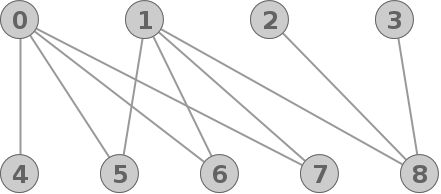
\includegraphics[scale = 0.2]{img/ej3/busqueda_local/k5,4Nocompleto_st0.png} &
			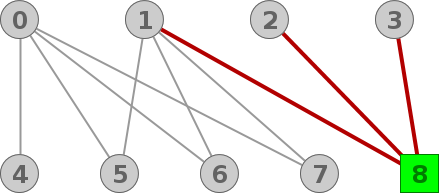
\includegraphics[scale = 0.2]{img/ej3/busqueda_local/k5,4Nocompleto_st1.png} & 
			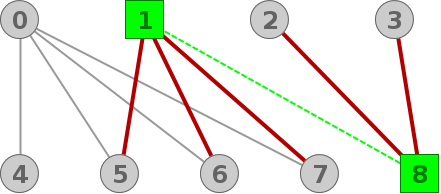
\includegraphics[scale = 0.2]{img/ej3/busqueda_local/k5,4Nocompleto_st2.png} \\
		\hline
		\end{tabular}
	\end{center}
\end{figure}
En este caso el grado promedio es $2,2$ con lo que podr\'ia suceder 
(con las etiquetas correctas) que la busqueda local comience con el
nodo marcado como $8$ en el ejemplo, cosa que en la golosa 
constructiva no pod\'ia suceder.

Para los \'arboles tambi\'en analizaremos el caso extremo presentado 
en la figura \ref{fig:extremo_arboles} y analizaremos nuevamente
la curiosidad de que debido a la relajaci\'on en el criterio de 
selecci\'on del primer nodo en busqueda local, existe una 
construccion alternativa de la clique devuelta por la heur\'istica
aunque sobre este ejemplo la respuesta ser\'a sub-optima.

\begin{figure}[H]
\caption{Resultado sub-\'optimo del ejemplo extremo para \'arboles - 
Forma alternativa}
\begin{center}
		\begin{tabular}{|c||c||c|}
		\hline
		Grafo de entrada & Paso 1 & Paso 2 \\ 
			\hline
			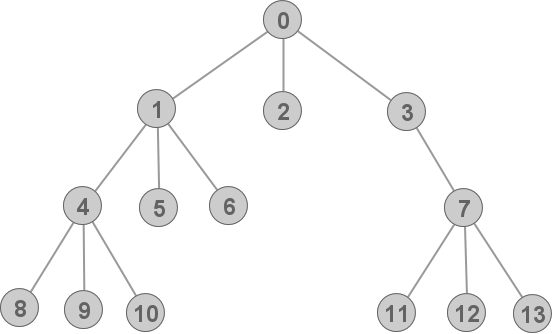
\includegraphics[scale = 0.2]{img/ej3/busqueda_local/extremetree_st0.png} &
			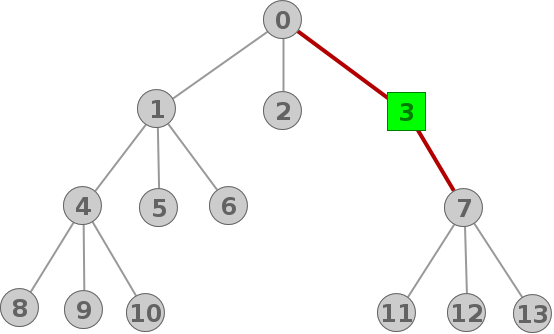
\includegraphics[scale = 0.2]{img/ej3/busqueda_local/extremetree_st11.png} & 
			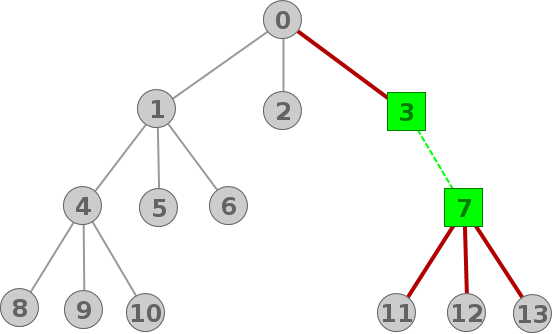
\includegraphics[scale = 0.2]{img/ej3/busqueda_local/extremetree_st12.png} \\
		\hline
		\end{tabular}
	\end{center}
\end{figure}
Notar que aqu\'i el grado promedio es aproximadamente $1,8$ con lo que 
el nodo identificado como $3$ en el ejemplo es elegible como
primer nodo de $K$ pues $2 > 1,8$.

\subsubsection{Estrella + Puente + CMF}

En esta familia, siguiendo con la idea de las \'ultimas dos analizadas
podemos ver que que para llegar a la soluci\'on \'optima hay muchos 
m\'as puntos de inicio que en la golosa constructiva. Por ejemplo
el primer nodo puede estar en $K_{\Delta -1}$ y no ser siquiera $v'$ 
(ver Figura \ref{fig:epcmf_carac}), en los casos en los que esto 
suceda, en la variante b\'asica, la busqueda local elegir\'a
$\left\lfloor \frac{\Delta -1}{2} \right\rfloor$ nodos de $K_{\Delta -1}$. 
Si estos nodos incluyen a $v'$, termina pues no quedan candidatos que
hagan crecer la soluci\'on parcial, si no lo incluyen hay dos posibilidades:

\begin{itemize}
	\item $\Delta$ par: La cantidad de nodos en $K_{\Delta -1}$ ser\'a impar 
	y entonces la soluci\'on crece hasta alcanzar
	$\left\lfloor \frac{\Delta -1}{2} \right\rfloor$ nodos que por hip\'otesis
	no incluyen a $v'$, en el siguiente paso el \'unico candidato restante
	que hace crecer la soluci\'on en una arista es $v'$ y por ello lo agrega 
	a la soluci\'on, terminando con una soluci\'on \'optima.
	\begin{center}
	\begin{tabular}{|c||c|}
		\hline
		Grafo entrada & 
		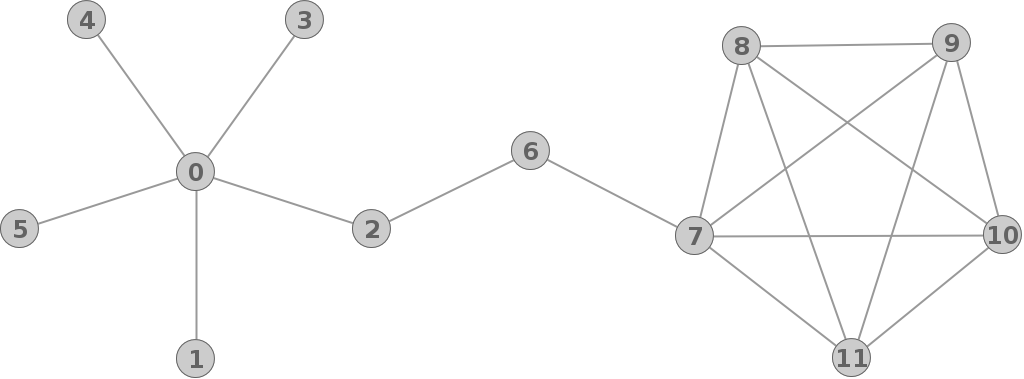
\includegraphics[scale = 0.2]{img/ej3/busqueda_local/estrellaPuenteCMFImpar.png} \\
		\hline
		Primer paso &
		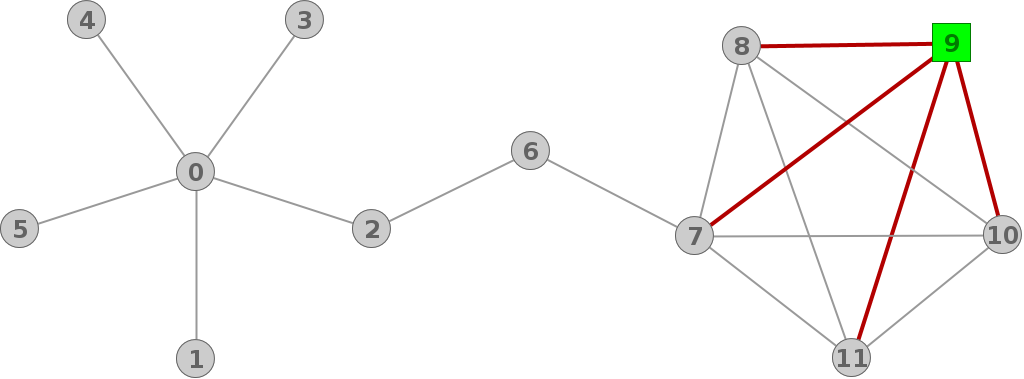
\includegraphics[scale = 0.2]{img/ej3/busqueda_local/estrellaPuenteCMFImpar_st01.png} \\
		\hline
		Segundo paso &
		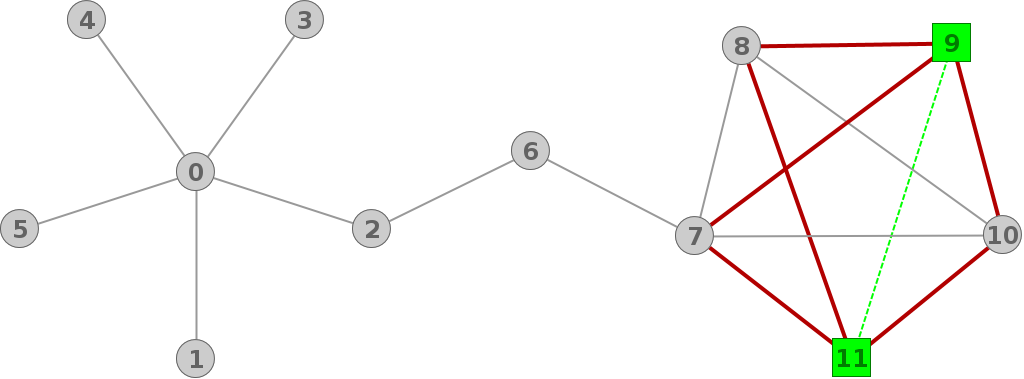
\includegraphics[scale = 0.2]{img/ej3/busqueda_local/estrellaPuenteCMFImpar_st02.png} \\
		\hline
		Tercer paso &
		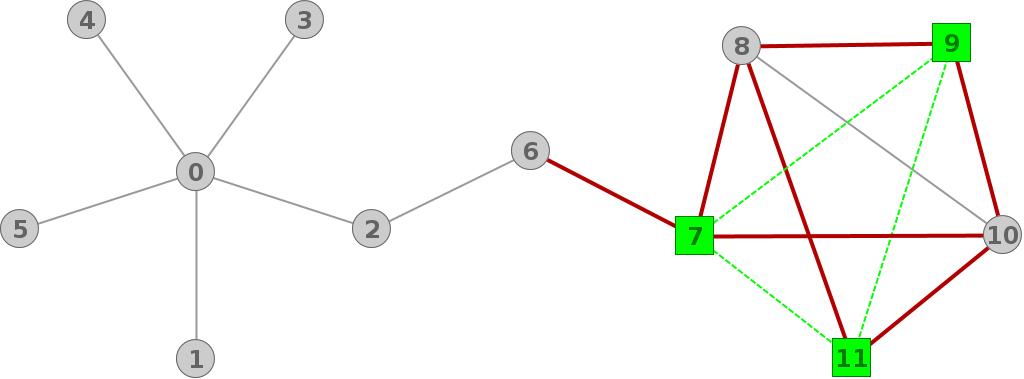
\includegraphics[scale = 0.2]{img/ej3/busqueda_local/estrellaPuenteCMFImpar_st03.png} \\
		\hline

	\end{tabular}
	\end{center}


	\item $\Delta$ impar: La cantidad de nodos en $K_{\Delta -1}$ ser\'a par, 
	en este caso la soluci\'on crece hasta alcanzar $\frac{\Delta -1}{2}$ nodos
	que no incluyen a $v'$, llegados a este punto la soluci\'on no puede crecer
	para incluir a $v'$ ya que de hacerlo la frontera de la soluci\'on ser\'ia
	la misma que en el paso anterior y el algoritmo no se comporta de esta manera.
	Por ende la soluci\'on devuelta es sub-\'optima.
	\begin{center}
	\begin{tabular}{|c||c|}
		\hline
		Grafo entrada & 
		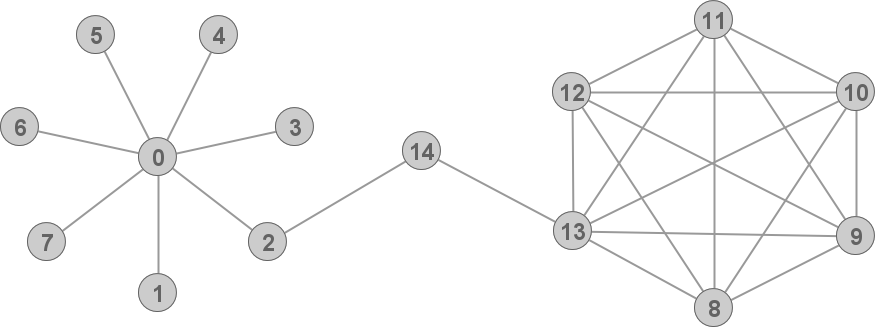
\includegraphics[scale = 0.2]{img/ej3/busqueda_local/estrellaPuenteCMFPar.png} \\
		\hline
		Primer paso &
		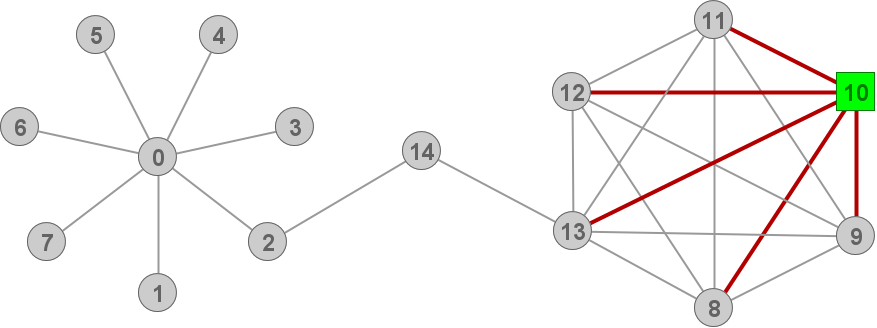
\includegraphics[scale = 0.2]{img/ej3/busqueda_local/estrellaPuenteCMFPar_st01.png} \\
		\hline
		Segundo paso &
		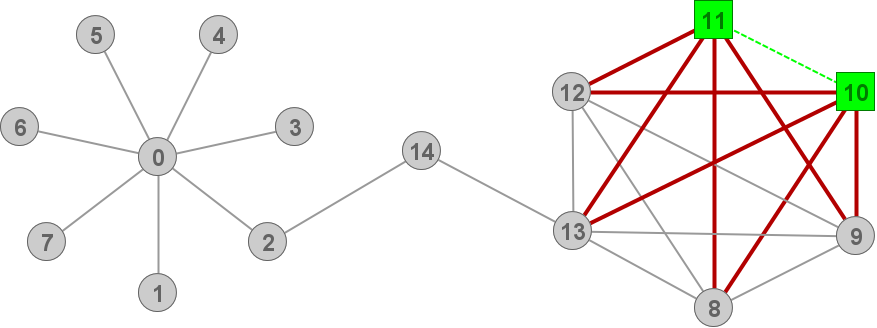
\includegraphics[scale = 0.2]{img/ej3/busqueda_local/estrellaPuenteCMFPar_st02.png} \\
		\hline
		Tercer paso &
		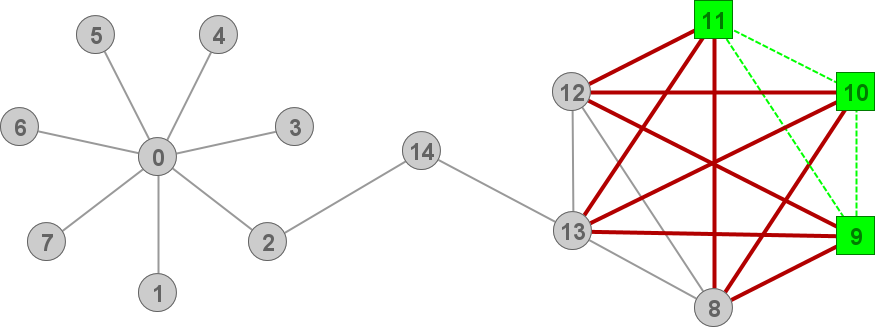
\includegraphics[scale = 0.2]{img/ej3/busqueda_local/estrellaPuenteCMFPar_st03.png} \\
		\hline

	\end{tabular}
	\end{center}


\end{itemize}

Notar que en la variante \emph{Mejor Vecino} evita el resultado sub-\'optimo en 
el \'ultimo caso (bajo las hip\'otesis del mismo).

Hay otros posibles comportamientos de la heur\'istica sobre la misma familia de
grafos, que el algoritmo comience la soluci\'on en uno de los nodos del puente o
que la comience en el centro de la estrella.

Que comience la soluci\'on sobre el puente es un caso que t\'ipicamente no va a 
suceder, si es un puente simple (camino simple) la \'unica forma de que sucediera
ser\'ia si el puente es lo suficientemente largo para bajar el grado promedio a
un valor menor a dos, si el puente no es un camino simple y en cambio tiene nodos
extra, el puente no tendr\'a que ser tan largo pero siempre se deber\'a cumplir
que el nodo inicial de la soluci\'on tenga grado mayor al grado promedio del grafo.

Cuando la soluci\'on se inicia en el centro de la estrella, la busqueda local 
se estanca en el m\'aximo local debido al puente que une la estrella con $K_{\Delta -1}$,
de hecho, esta familia fue dise\~nada con el objetivo de asegurar precisamente
este estancamiento.
		



\subsection{Experimentaci\'on}
    \subsubsection{Resultados}
\par Se presentan a continuaci\'on los resultados de la experimentaci\'on
    de la heur\'istica golosa constructiva para \emph{CMF}. La experimentaci\'on se realiz\'o
    con las instancias ya generadas (seg\'un se explica en \emph{\nameref{notas_preliminares},
    \nameref{notas:datasets}} y \emph{\nameref{notas:experimentacion}}).

\par Para recordar, se cuentan con 10 instancias aleatorias de cada tama\~no,
    las cuales fueron resueltas 5 veces cada una y nos quedamos con el menor tiempo
    requerido de esas 5 ejecuciones. Por \'ultimo, tomamos el promedio de este tiempo
    requerido calculado entre las instancias del mismo tama\~no (10, como se ha
    dicho).

\bigskip

\begin{figure}[H]
    \centering
    \fontsize{8}{10}\selectfont
    \resizebox{0.8\textwidth}{!}{% GNUPLOT: LaTeX picture with Postscript
\begingroup
  \makeatletter
  \providecommand\color[2][]{%
    \GenericError{(gnuplot) \space\space\space\@spaces}{%
      Package color not loaded in conjunction with
      terminal option `colourtext'%
    }{See the gnuplot documentation for explanation.%
    }{Either use 'blacktext' in gnuplot or load the package
      color.sty in LaTeX.}%
    \renewcommand\color[2][]{}%
  }%
  \providecommand\includegraphics[2][]{%
    \GenericError{(gnuplot) \space\space\space\@spaces}{%
      Package graphicx or graphics not loaded%
    }{See the gnuplot documentation for explanation.%
    }{The gnuplot epslatex terminal needs graphicx.sty or graphics.sty.}%
    \renewcommand\includegraphics[2][]{}%
  }%
  \providecommand\rotatebox[2]{#2}%
  \@ifundefined{ifGPcolor}{%
    \newif\ifGPcolor
    \GPcolortrue
  }{}%
  \@ifundefined{ifGPblacktext}{%
    \newif\ifGPblacktext
    \GPblacktexttrue
  }{}%
  % define a \g@addto@macro without @ in the name:
  \let\gplgaddtomacro\g@addto@macro
  % define empty templates for all commands taking text:
  \gdef\gplbacktext{}%
  \gdef\gplfronttext{}%
  \makeatother
  \ifGPblacktext
    % no textcolor at all
    \def\colorrgb#1{}%
    \def\colorgray#1{}%
  \else
    % gray or color?
    \ifGPcolor
      \def\colorrgb#1{\color[rgb]{#1}}%
      \def\colorgray#1{\color[gray]{#1}}%
      \expandafter\def\csname LTw\endcsname{\color{white}}%
      \expandafter\def\csname LTb\endcsname{\color{black}}%
      \expandafter\def\csname LTa\endcsname{\color{black}}%
      \expandafter\def\csname LT0\endcsname{\color[rgb]{1,0,0}}%
      \expandafter\def\csname LT1\endcsname{\color[rgb]{0,1,0}}%
      \expandafter\def\csname LT2\endcsname{\color[rgb]{0,0,1}}%
      \expandafter\def\csname LT3\endcsname{\color[rgb]{1,0,1}}%
      \expandafter\def\csname LT4\endcsname{\color[rgb]{0,1,1}}%
      \expandafter\def\csname LT5\endcsname{\color[rgb]{1,1,0}}%
      \expandafter\def\csname LT6\endcsname{\color[rgb]{0,0,0}}%
      \expandafter\def\csname LT7\endcsname{\color[rgb]{1,0.3,0}}%
      \expandafter\def\csname LT8\endcsname{\color[rgb]{0.5,0.5,0.5}}%
    \else
      % gray
      \def\colorrgb#1{\color{black}}%
      \def\colorgray#1{\color[gray]{#1}}%
      \expandafter\def\csname LTw\endcsname{\color{white}}%
      \expandafter\def\csname LTb\endcsname{\color{black}}%
      \expandafter\def\csname LTa\endcsname{\color{black}}%
      \expandafter\def\csname LT0\endcsname{\color{black}}%
      \expandafter\def\csname LT1\endcsname{\color{black}}%
      \expandafter\def\csname LT2\endcsname{\color{black}}%
      \expandafter\def\csname LT3\endcsname{\color{black}}%
      \expandafter\def\csname LT4\endcsname{\color{black}}%
      \expandafter\def\csname LT5\endcsname{\color{black}}%
      \expandafter\def\csname LT6\endcsname{\color{black}}%
      \expandafter\def\csname LT7\endcsname{\color{black}}%
      \expandafter\def\csname LT8\endcsname{\color{black}}%
    \fi
  \fi
  \setlength{\unitlength}{0.0500bp}%
  \begin{picture}(7200.00,5040.00)%
    \gplgaddtomacro\gplbacktext{%
      \csname LTb\endcsname%
      \put(1430,2244){\makebox(0,0)[r]{\strut{} 0}}%
      \csname LTb\endcsname%
      \put(1430,2549){\makebox(0,0)[r]{\strut{} 5000}}%
      \csname LTb\endcsname%
      \put(1430,2854){\makebox(0,0)[r]{\strut{} 10000}}%
      \csname LTb\endcsname%
      \put(1430,3159){\makebox(0,0)[r]{\strut{} 15000}}%
      \csname LTb\endcsname%
      \put(1430,3464){\makebox(0,0)[r]{\strut{} 20000}}%
      \csname LTb\endcsname%
      \put(1430,3769){\makebox(0,0)[r]{\strut{} 25000}}%
      \csname LTb\endcsname%
      \put(1430,4074){\makebox(0,0)[r]{\strut{} 30000}}%
      \csname LTb\endcsname%
      \put(1430,4379){\makebox(0,0)[r]{\strut{} 35000}}%
      \csname LTb\endcsname%
      \put(1562,2024){\makebox(0,0){\strut{} 0}}%
      \csname LTb\endcsname%
      \put(2086,2024){\makebox(0,0){\strut{} 500}}%
      \csname LTb\endcsname%
      \put(2610,2024){\makebox(0,0){\strut{} 1000}}%
      \csname LTb\endcsname%
      \put(3134,2024){\makebox(0,0){\strut{} 1500}}%
      \csname LTb\endcsname%
      \put(3658,2024){\makebox(0,0){\strut{} 2000}}%
      \csname LTb\endcsname%
      \put(4183,2024){\makebox(0,0){\strut{} 2500}}%
      \csname LTb\endcsname%
      \put(4707,2024){\makebox(0,0){\strut{} 3000}}%
      \csname LTb\endcsname%
      \put(5231,2024){\makebox(0,0){\strut{} 3500}}%
      \csname LTb\endcsname%
      \put(5755,2024){\makebox(0,0){\strut{} 4000}}%
      \csname LTb\endcsname%
      \put(6279,2024){\makebox(0,0){\strut{} 4500}}%
      \csname LTb\endcsname%
      \put(6803,2024){\makebox(0,0){\strut{} 5000}}%
      \put(176,3311){\rotatebox{-270}{\makebox(0,0){\strut{}Tiempo (nanosegundos)}}}%
      \put(396,3311){\rotatebox{-270}{\makebox(0,0){\strut{}(Escala Lineal)}}}%
      \put(4182,1694){\makebox(0,0){\strut{}Cantidad de Nodos}}%
      \put(4182,1474){\makebox(0,0){\strut{}(Escala Lineal)}}%
      \put(4182,4709){\makebox(0,0){\strut{}Tiempo de ejecución conforme aumenta la cantidad de nodos}}%
    }%
    \gplgaddtomacro\gplfronttext{%
      \csname LTb\endcsname%
      \put(5735,1053){\makebox(0,0)[r]{\strut{}Grafos Completos}}%
      \csname LTb\endcsname%
      \put(5735,833){\makebox(0,0)[r]{\strut{}Arboles}}%
      \csname LTb\endcsname%
      \put(5735,613){\makebox(0,0)[r]{\strut{}Circulares}}%
      \csname LTb\endcsname%
      \put(5735,393){\makebox(0,0)[r]{\strut{}Cota teórica superior $\mathcal O(n^2)$}}%
      \csname LTb\endcsname%
      \put(5735,173){\makebox(0,0)[r]{\strut{}Cota teórica superior $\mathcal O(n)$}}%
    }%
    \gplbacktext
    \put(0,0){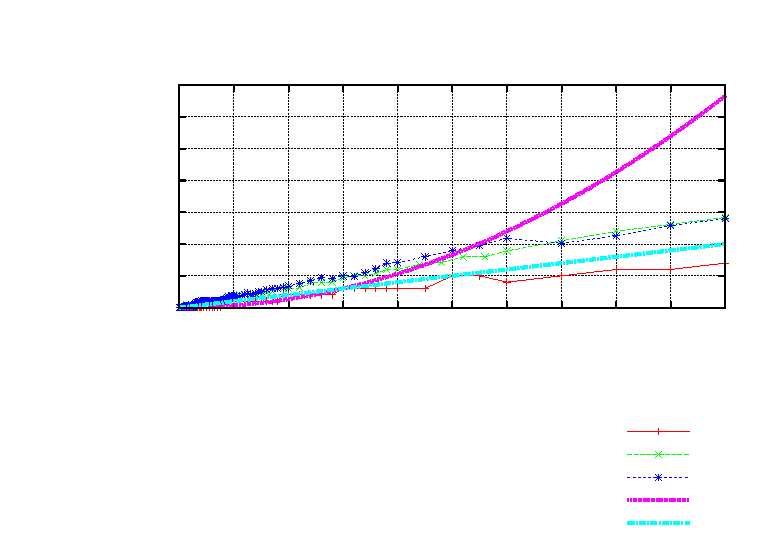
\includegraphics{ej3_nodos_completos_arboles_circulares}}%
    \gplfronttext
  \end{picture}%
\endgroup
}
    \caption{Complejidad temporal para grafos completos, \'arboles y circulares}
\end{figure}

\begin{figure}[H]
    \centering
    \fontsize{8}{10}\selectfont
    \resizebox{0.8\textwidth}{!}{% GNUPLOT: LaTeX picture with Postscript
\begingroup
  \makeatletter
  \providecommand\color[2][]{%
    \GenericError{(gnuplot) \space\space\space\@spaces}{%
      Package color not loaded in conjunction with
      terminal option `colourtext'%
    }{See the gnuplot documentation for explanation.%
    }{Either use 'blacktext' in gnuplot or load the package
      color.sty in LaTeX.}%
    \renewcommand\color[2][]{}%
  }%
  \providecommand\includegraphics[2][]{%
    \GenericError{(gnuplot) \space\space\space\@spaces}{%
      Package graphicx or graphics not loaded%
    }{See the gnuplot documentation for explanation.%
    }{The gnuplot epslatex terminal needs graphicx.sty or graphics.sty.}%
    \renewcommand\includegraphics[2][]{}%
  }%
  \providecommand\rotatebox[2]{#2}%
  \@ifundefined{ifGPcolor}{%
    \newif\ifGPcolor
    \GPcolortrue
  }{}%
  \@ifundefined{ifGPblacktext}{%
    \newif\ifGPblacktext
    \GPblacktexttrue
  }{}%
  % define a \g@addto@macro without @ in the name:
  \let\gplgaddtomacro\g@addto@macro
  % define empty templates for all commands taking text:
  \gdef\gplbacktext{}%
  \gdef\gplfronttext{}%
  \makeatother
  \ifGPblacktext
    % no textcolor at all
    \def\colorrgb#1{}%
    \def\colorgray#1{}%
  \else
    % gray or color?
    \ifGPcolor
      \def\colorrgb#1{\color[rgb]{#1}}%
      \def\colorgray#1{\color[gray]{#1}}%
      \expandafter\def\csname LTw\endcsname{\color{white}}%
      \expandafter\def\csname LTb\endcsname{\color{black}}%
      \expandafter\def\csname LTa\endcsname{\color{black}}%
      \expandafter\def\csname LT0\endcsname{\color[rgb]{1,0,0}}%
      \expandafter\def\csname LT1\endcsname{\color[rgb]{0,1,0}}%
      \expandafter\def\csname LT2\endcsname{\color[rgb]{0,0,1}}%
      \expandafter\def\csname LT3\endcsname{\color[rgb]{1,0,1}}%
      \expandafter\def\csname LT4\endcsname{\color[rgb]{0,1,1}}%
      \expandafter\def\csname LT5\endcsname{\color[rgb]{1,1,0}}%
      \expandafter\def\csname LT6\endcsname{\color[rgb]{0,0,0}}%
      \expandafter\def\csname LT7\endcsname{\color[rgb]{1,0.3,0}}%
      \expandafter\def\csname LT8\endcsname{\color[rgb]{0.5,0.5,0.5}}%
    \else
      % gray
      \def\colorrgb#1{\color{black}}%
      \def\colorgray#1{\color[gray]{#1}}%
      \expandafter\def\csname LTw\endcsname{\color{white}}%
      \expandafter\def\csname LTb\endcsname{\color{black}}%
      \expandafter\def\csname LTa\endcsname{\color{black}}%
      \expandafter\def\csname LT0\endcsname{\color{black}}%
      \expandafter\def\csname LT1\endcsname{\color{black}}%
      \expandafter\def\csname LT2\endcsname{\color{black}}%
      \expandafter\def\csname LT3\endcsname{\color{black}}%
      \expandafter\def\csname LT4\endcsname{\color{black}}%
      \expandafter\def\csname LT5\endcsname{\color{black}}%
      \expandafter\def\csname LT6\endcsname{\color{black}}%
      \expandafter\def\csname LT7\endcsname{\color{black}}%
      \expandafter\def\csname LT8\endcsname{\color{black}}%
    \fi
  \fi
  \setlength{\unitlength}{0.0500bp}%
  \begin{picture}(7200.00,5040.00)%
    \gplgaddtomacro\gplbacktext{%
      \csname LTb\endcsname%
      \put(1166,2244){\makebox(0,0)[r]{\strut{} 0}}%
      \csname LTb\endcsname%
      \put(1166,2511){\makebox(0,0)[r]{\strut{} 100}}%
      \csname LTb\endcsname%
      \put(1166,2778){\makebox(0,0)[r]{\strut{} 200}}%
      \csname LTb\endcsname%
      \put(1166,3045){\makebox(0,0)[r]{\strut{} 300}}%
      \csname LTb\endcsname%
      \put(1166,3312){\makebox(0,0)[r]{\strut{} 400}}%
      \csname LTb\endcsname%
      \put(1166,3578){\makebox(0,0)[r]{\strut{} 500}}%
      \csname LTb\endcsname%
      \put(1166,3845){\makebox(0,0)[r]{\strut{} 600}}%
      \csname LTb\endcsname%
      \put(1166,4112){\makebox(0,0)[r]{\strut{} 700}}%
      \csname LTb\endcsname%
      \put(1166,4379){\makebox(0,0)[r]{\strut{} 800}}%
      \csname LTb\endcsname%
      \put(1298,2024){\makebox(0,0){\strut{} 0}}%
      \csname LTb\endcsname%
      \put(1849,2024){\makebox(0,0){\strut{} 500}}%
      \csname LTb\endcsname%
      \put(2399,2024){\makebox(0,0){\strut{} 1000}}%
      \csname LTb\endcsname%
      \put(2950,2024){\makebox(0,0){\strut{} 1500}}%
      \csname LTb\endcsname%
      \put(3500,2024){\makebox(0,0){\strut{} 2000}}%
      \csname LTb\endcsname%
      \put(4051,2024){\makebox(0,0){\strut{} 2500}}%
      \csname LTb\endcsname%
      \put(4601,2024){\makebox(0,0){\strut{} 3000}}%
      \csname LTb\endcsname%
      \put(5152,2024){\makebox(0,0){\strut{} 3500}}%
      \csname LTb\endcsname%
      \put(5702,2024){\makebox(0,0){\strut{} 4000}}%
      \csname LTb\endcsname%
      \put(6253,2024){\makebox(0,0){\strut{} 4500}}%
      \csname LTb\endcsname%
      \put(6803,2024){\makebox(0,0){\strut{} 5000}}%
      \put(176,3311){\rotatebox{-270}{\makebox(0,0){\strut{}Tiempo (microsegundos)}}}%
      \put(396,3311){\rotatebox{-270}{\makebox(0,0){\strut{}(Escala Lineal)}}}%
      \put(4050,1694){\makebox(0,0){\strut{}Cantidad de Nodos}}%
      \put(4050,1474){\makebox(0,0){\strut{}(Escala Lineal)}}%
      \put(4050,4709){\makebox(0,0){\strut{}Tiempo de ejecución conforme aumenta la cantidad de nodos}}%
    }%
    \gplgaddtomacro\gplfronttext{%
      \csname LTb\endcsname%
      \put(5603,1053){\makebox(0,0)[r]{\strut{}Estrellas}}%
      \csname LTb\endcsname%
      \put(5603,833){\makebox(0,0)[r]{\strut{}Ruedas}}%
      \csname LTb\endcsname%
      \put(5603,613){\makebox(0,0)[r]{\strut{}Banana Tree}}%
      \csname LTb\endcsname%
      \put(5603,393){\makebox(0,0)[r]{\strut{}Bipartitos}}%
      \csname LTb\endcsname%
      \put(5603,173){\makebox(0,0)[r]{\strut{}Cota teórica superior $\mathcal O(n^2)$}}%
    }%
    \gplbacktext
    \put(0,0){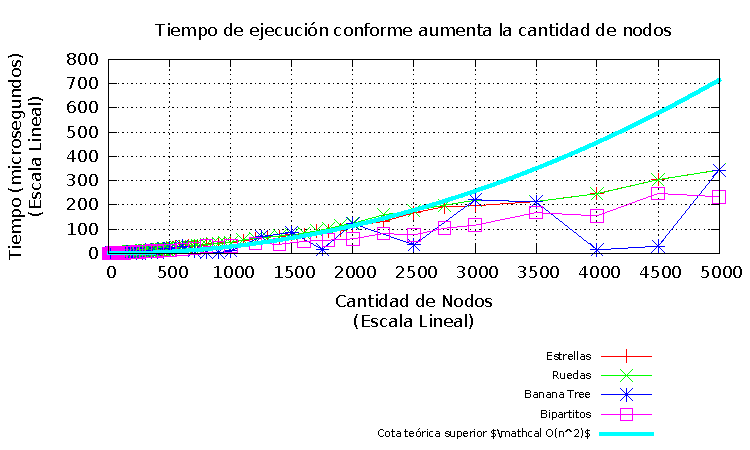
\includegraphics{ej3_nodos_estrella_rueda_banana_bipartito}}%
    \gplfronttext
  \end{picture}%
\endgroup
}
    \caption{Complejidad temporal para grafos estrella, rueda, banana tree y bipartitos}
\end{figure}

\begin{figure}[H]
    \centering
    \fontsize{8}{10}\selectfont
    \resizebox{0.8\textwidth}{!}{% GNUPLOT: LaTeX picture with Postscript
\begingroup
  \makeatletter
  \providecommand\color[2][]{%
    \GenericError{(gnuplot) \space\space\space\@spaces}{%
      Package color not loaded in conjunction with
      terminal option `colourtext'%
    }{See the gnuplot documentation for explanation.%
    }{Either use 'blacktext' in gnuplot or load the package
      color.sty in LaTeX.}%
    \renewcommand\color[2][]{}%
  }%
  \providecommand\includegraphics[2][]{%
    \GenericError{(gnuplot) \space\space\space\@spaces}{%
      Package graphicx or graphics not loaded%
    }{See the gnuplot documentation for explanation.%
    }{The gnuplot epslatex terminal needs graphicx.sty or graphics.sty.}%
    \renewcommand\includegraphics[2][]{}%
  }%
  \providecommand\rotatebox[2]{#2}%
  \@ifundefined{ifGPcolor}{%
    \newif\ifGPcolor
    \GPcolortrue
  }{}%
  \@ifundefined{ifGPblacktext}{%
    \newif\ifGPblacktext
    \GPblacktexttrue
  }{}%
  % define a \g@addto@macro without @ in the name:
  \let\gplgaddtomacro\g@addto@macro
  % define empty templates for all commands taking text:
  \gdef\gplbacktext{}%
  \gdef\gplfronttext{}%
  \makeatother
  \ifGPblacktext
    % no textcolor at all
    \def\colorrgb#1{}%
    \def\colorgray#1{}%
  \else
    % gray or color?
    \ifGPcolor
      \def\colorrgb#1{\color[rgb]{#1}}%
      \def\colorgray#1{\color[gray]{#1}}%
      \expandafter\def\csname LTw\endcsname{\color{white}}%
      \expandafter\def\csname LTb\endcsname{\color{black}}%
      \expandafter\def\csname LTa\endcsname{\color{black}}%
      \expandafter\def\csname LT0\endcsname{\color[rgb]{1,0,0}}%
      \expandafter\def\csname LT1\endcsname{\color[rgb]{0,1,0}}%
      \expandafter\def\csname LT2\endcsname{\color[rgb]{0,0,1}}%
      \expandafter\def\csname LT3\endcsname{\color[rgb]{1,0,1}}%
      \expandafter\def\csname LT4\endcsname{\color[rgb]{0,1,1}}%
      \expandafter\def\csname LT5\endcsname{\color[rgb]{1,1,0}}%
      \expandafter\def\csname LT6\endcsname{\color[rgb]{0,0,0}}%
      \expandafter\def\csname LT7\endcsname{\color[rgb]{1,0.3,0}}%
      \expandafter\def\csname LT8\endcsname{\color[rgb]{0.5,0.5,0.5}}%
    \else
      % gray
      \def\colorrgb#1{\color{black}}%
      \def\colorgray#1{\color[gray]{#1}}%
      \expandafter\def\csname LTw\endcsname{\color{white}}%
      \expandafter\def\csname LTb\endcsname{\color{black}}%
      \expandafter\def\csname LTa\endcsname{\color{black}}%
      \expandafter\def\csname LT0\endcsname{\color{black}}%
      \expandafter\def\csname LT1\endcsname{\color{black}}%
      \expandafter\def\csname LT2\endcsname{\color{black}}%
      \expandafter\def\csname LT3\endcsname{\color{black}}%
      \expandafter\def\csname LT4\endcsname{\color{black}}%
      \expandafter\def\csname LT5\endcsname{\color{black}}%
      \expandafter\def\csname LT6\endcsname{\color{black}}%
      \expandafter\def\csname LT7\endcsname{\color{black}}%
      \expandafter\def\csname LT8\endcsname{\color{black}}%
    \fi
  \fi
  \setlength{\unitlength}{0.0500bp}%
  \begin{picture}(7200.00,5040.00)%
    \gplgaddtomacro\gplbacktext{%
      \csname LTb\endcsname%
      \put(1166,1804){\makebox(0,0)[r]{\strut{} 0}}%
      \csname LTb\endcsname%
      \put(1166,2090){\makebox(0,0)[r]{\strut{} 50}}%
      \csname LTb\endcsname%
      \put(1166,2376){\makebox(0,0)[r]{\strut{} 100}}%
      \csname LTb\endcsname%
      \put(1166,2662){\makebox(0,0)[r]{\strut{} 150}}%
      \csname LTb\endcsname%
      \put(1166,2948){\makebox(0,0)[r]{\strut{} 200}}%
      \csname LTb\endcsname%
      \put(1166,3235){\makebox(0,0)[r]{\strut{} 250}}%
      \csname LTb\endcsname%
      \put(1166,3521){\makebox(0,0)[r]{\strut{} 300}}%
      \csname LTb\endcsname%
      \put(1166,3807){\makebox(0,0)[r]{\strut{} 350}}%
      \csname LTb\endcsname%
      \put(1166,4093){\makebox(0,0)[r]{\strut{} 400}}%
      \csname LTb\endcsname%
      \put(1166,4379){\makebox(0,0)[r]{\strut{} 450}}%
      \csname LTb\endcsname%
      \put(1298,1584){\makebox(0,0){\strut{} 0}}%
      \csname LTb\endcsname%
      \put(1849,1584){\makebox(0,0){\strut{} 500}}%
      \csname LTb\endcsname%
      \put(2399,1584){\makebox(0,0){\strut{} 1000}}%
      \csname LTb\endcsname%
      \put(2950,1584){\makebox(0,0){\strut{} 1500}}%
      \csname LTb\endcsname%
      \put(3500,1584){\makebox(0,0){\strut{} 2000}}%
      \csname LTb\endcsname%
      \put(4051,1584){\makebox(0,0){\strut{} 2500}}%
      \csname LTb\endcsname%
      \put(4601,1584){\makebox(0,0){\strut{} 3000}}%
      \csname LTb\endcsname%
      \put(5152,1584){\makebox(0,0){\strut{} 3500}}%
      \csname LTb\endcsname%
      \put(5702,1584){\makebox(0,0){\strut{} 4000}}%
      \csname LTb\endcsname%
      \put(6253,1584){\makebox(0,0){\strut{} 4500}}%
      \csname LTb\endcsname%
      \put(6803,1584){\makebox(0,0){\strut{} 5000}}%
      \put(176,3091){\rotatebox{-270}{\makebox(0,0){\strut{}Tiempo (microsegundos)}}}%
      \put(396,3091){\rotatebox{-270}{\makebox(0,0){\strut{}(Escala Lineal)}}}%
      \put(4050,1254){\makebox(0,0){\strut{}Cantidad de Nodos}}%
      \put(4050,1034){\makebox(0,0){\strut{}(Escala Lineal)}}%
      \put(4050,4709){\makebox(0,0){\strut{}Tiempo de ejecución conforme aumenta la cantidad de nodos}}%
    }%
    \gplgaddtomacro\gplfronttext{%
      \csname LTb\endcsname%
      \put(5603,613){\makebox(0,0)[r]{\strut{}Estrella+CMF}}%
      \csname LTb\endcsname%
      \put(5603,393){\makebox(0,0)[r]{\strut{}Estrella+Puente+CMF}}%
      \csname LTb\endcsname%
      \put(5603,173){\makebox(0,0)[r]{\strut{}Cota teórica superior $\mathcal O(n^2)$}}%
    }%
    \gplbacktext
    \put(0,0){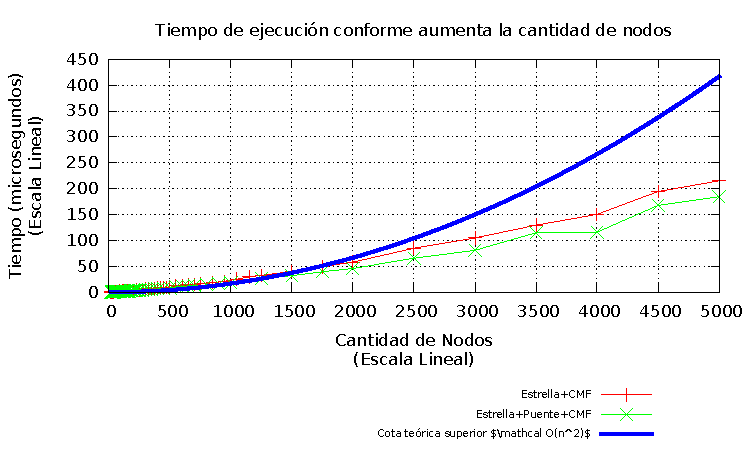
\includegraphics{ej3_nodos_disruptivas}}%
    \gplfronttext
  \end{picture}%
\endgroup
}
    \caption{Complejidad temporal para grafos Estrella+CMF, Estrella+Puente+CMF}
\end{figure}

\subsubsection{Conclusiones}
\par En los primeros 2 resultados se puede observar que la complejidad asint\'otica
    para las familias ``simples''\footnote{Consideramos a los grafos completos
    como una familia simple pues con los datos de entrada resolver el problema
    de \emph{CMF} es trivial.} (pocas aristas y con estructuras muy restrictivas)
    es similar. Si bien hay diferencias (en el orden de los nanosegundos), se
    destaca que todas cumplen con la complejidad asint\'otica temporal te\'orica
    calculada y a su vez se comportan de la misma manera en cuanto a crecimiento.

\par En el segundo gr\'afico, tambi\'en se cuentan con una serie de familias
    ``simples'', pero aqu\'i el comportamiento de nuestra heur\'istica resulta
    un tanto m\'as err\'atico, si bien sigue estando en el orden de complejidad
    calculado. Se puede observar que mientras que las familias de las 
    Rueadas y las estrellas (de estructuras muy similares) se comportan pr\'acticamente
    igual, para los grafos bipartitos se requiere menor tiempo para resolver
    instancias del mismo tama\~no. Esto es un tanto raro, ya que en las 3 familias
    (como ya se ha explicado) la \emph{CMF} tendr\'a el mismo tama\~no. S\'olo
    nos queda hipotetizar\footnote{Viernes 22 de Noviembre, 17:58 hs GMT-3} sobre los motivos.

\par En el caso de la familia de grafos \emph{Banana Tree}, suponemos que su comportamiento
    se debe que seg\'un el tama\~no de las estrellas que tenga en sus extremos, el nodo
    de mayor grado estar\'a en alguna estrella o en el nodo central que une a todas las estrellas.
    Este dato tendr\'a una influencia inmediata en la elecci\'on de los nodos candidatos
    a agregarse a la clique luego de haber encontrado el nodo de mayor grado del grafo (ya
    que si las estrellas/extremidades son de tama\~no considerable, las mismas
    deberan ser tenidas en cuenta, mientras que si solo se tiene una gran estrella (las
    ``bananas'' son de taman\~o 1), esto ser\'a m\'as eficiente.

\par Por \'ultimo, observamos que el comportamiento para las familias Estrella+CMF y
    Estrella+Puente+CMF es muy estable a medida que crece el taman\~o de las instancias.
    Quiz\'as lo m\'as interesantes de estas familias (aparte de comprobar que cumplen
    con la complejidad asint\'otica te\'orica) es comparar los resultados otorgados
    por la heur\'istica con el algoritmo exacto u las dem\'as heur\'isticas. Esto
    se efectua en la Secci\'on~\ref{experimentacion} de este trabajo.


        \pagebreak

    \section{Heur\'istica de B\'usqueda Local}
        \subsection{Resoluci\'on}
    \begin{algorithm}[H]
    \caption{Heur\'istica Golosa Constructiva 1 para \emph{CMF} - Descriptivo}
    \begin{algorithmic}[1]
        \Require\Statex
            \begin{itemize}
                \item Un grafo $G$ de $n$ v\'ertices y $m$ aristas.

                \item Una funci\'on $candidatos(K)$, que dado un conjunto de v\'ertices
                    $K$, devuelve el conjunto de v\'ertices de $G$ que son adjacentes
                    a todos los elementos de $K$, cuyo grado es mayor $2|K|$.
            \end{itemize}

        \Statex

        \Ensure Una \emph{clique} $K$ de $G$ con una frontera $\delta(K)$ que se
            espera que sea de cardinalidad cercana o igual a la de $\delta(K')$,
            siendo $K'$ la \emph{clique} de m\'axima frontera de $G$.

        \Statex

        \State Sea $v$ el v\'ertice de mayor grado en $G$.
        \State $K \gets \{v\}$
        \While{$candidatos(K) \neq \emptyset$}
            \State Sea $v'$ el v\'ertice de mayor grado en $candidatos(K)$.
            \State $K \gets K \cup \{v'\}$
        \EndWhile

        \State \Return{$K$}
    \end{algorithmic}
\end{algorithm}

\begin{algorithm}[H]
    \caption{Heur\'istica Golosa Constructiva 2 para \emph{CMF} - Descriptivo}
    \begin{algorithmic}[1]
        \Require Un grafo $G$ de $n$ v\'ertices y $m$ aristas.
        \Ensure Una \emph{clique} $K$ de $G$ con una frontera $\delta(K)$ que se
            espera que sea de cardinalidad cercana o igual a la de $\delta(K')$,
            siendo $K'$ la \emph{clique} de m\'axima frontera de $G$.

        \Statex

        \State $K \gets \emptyset$
        \State $\delta_{max} \gets 0$
        \State $Ks \gets $ Todos los conjuntos de 2 o 3 v\'ertices de $G$ que
            forman una \emph{clique}.
        \ForEach{$K' \in Ks$}
            \If{$\delta(K') > \delta_{max}$}
                \State $\delta_{max} \gets \delta(K')$
                \State $K \gets K'$

            \EndIf

        \EndForEach

        \State \Return{$K$}
    \end{algorithmic}
\end{algorithm}


\subsection{Complejidad}
    \subsubsection{Estructuras de Datos}

\subsubsection{Pseudoc\'odigo de complejidad}
\par Se presenta a continuaci\'on un pseudoc\'odigo m\'as espec\'ifico de la implementaci\'on
    de este algoritmo provista junto con este trabajo. El mismo tiene en cuenta
    las estructuras de datos explicadas en el punto anterior.

\par Luego del pseudoc\'odigo se justifican detalladamente las complejidades
    expuestas a continuaci\'on que no sean evidentes\footnote{Consideramos
    como "complejidades evidentes" las asignaciones de variables, operaciones
    m\'atematicas simples, asignaciones/inicializaci\'on de posiciones de
    un vector/\emph{deque} o cualquier contenedor de acceso aleatorio/arbitrario}.

\bigskip

\begin{pseudocodigo}[Heur\'istica de B\'usqueda Local para \emph{CMF} - Complejidad]
    \Require Un grafo $G$ con $n$ v\'ertices numerados de $1$ a $n$ y $m$ aristas. El mismo
        cuenta con las siguientes estructuras de datos que lo modelan:
        \begin{itemize}
            \item Vectores de adyacencia: Dado un vertice $v$, $vecinos(v)$ nos da todos los
                nodos adyacentes a $v$ en $G$.

            \item Matriz de adyacencia: Dados los v\'ertices $v$ y $w$, $adyacentes(v,w)$ y
                $adyacentes(w,v)$ nos devuelven $true$ si y s\'olo si $v$ es adyacente
                a $w$ en $G$.

            \item Vector de nodos de $G$.
        \end{itemize}
    \Ensure\Statex
        \begin{itemize}
            \item Un vector $K$ correspondiente a la \emph{clique} de m\'axima frontera
                encontrada por la heur\'istica.

            \item El cardinal de $\delta(K)$, siendo $K$ la \emph{clique} del item anterior.
        \end{itemize}
    \Statex

    \State $K \gets \emptyset$ \Compl{Brown}{}{$n$}{}
    \If{$m = \frac{n(n-1)}{2}$} \Compl{Blue}{}{$1$}{}
        \State $K \gets \left\{1;\dots;\left\lfloor\sfrac{n}{2}\right\rfloor\right\}$ \Compl{Blue}{}{$n$}{}
        \State $\delta_{max} \gets \left\lfloor\sfrac{n}{2}\right\rfloor\cdot
            \left\lceil\sfrac{n}{2}\right\rceil$ \Compl{Blue}{}{$1$}{}
        \Statex

    \Else
    \EndIf \Compl{Brown}{Costo \emph{si}: }{}{}

    \State \Return{$\delta(K)$, $K$} \Compl{Brown}{}{$1$\label{bl:return}}{}
    \Statex
    \Statex \Compl{Brown}{Costo Total de la Heur\'istica: }{}{}
\end{pseudocodigo}

\bigskip

\par


\subsection{Casos Particulares de Estudio}
    En lo que sigue haremos un somero estudio de ciertas familias
para intentar anticipar los resultados arrojados en la etapa
de experimentaci\'on. El estudio an\'alitico ser\'a m\'inimo
con lo que se dejar\'an muchas alternativas fuera del mismo,
la idea es que en etapa de experimentaci\'on puedan verse
generalizaciones de lo que analicemos en esta etapa.

En general los an\'alisis se efectuaran sobre la heur\'istica
original, no sobre sus alternativas, excepto en los casos en 
los que a simple vista, tomar en cuenta las mismas arroje
resultados f\'acilmente analizables e intersantes a priori.

Retomaremos aqu\'i las familias especificadas para el estudio
de la heur\'istica golosa constructiva con el proposito de 
comparar a nivel anal\'itico en qu\'e casos la heur\'istica
de busqueda local funciona mejor, peor o igual que la constructiva
golosa, esto es a nivel resultado \'optimo versus resultado
sub-\'optimo.

Hay ciertas familias de las especificadas anteriormente para
las que no vale la pena ser demasiado puntillosos. 
Por ejemplo la familia de grafos completos, ya desde la 
descripci\'on del algoritmo de busqueda local puede verse que 
siempre devuelve un resultado \'optimo, ya que cualesquiera
$\left\lfloor \frac{n}{2} \right\rfloor$ nodos son un 
resultado \'optimo y escogerlos de este modo es exactamente 
lo que hace nuestra heur\'istica.

Los otros casos para los que la golosa funcionaba bien: estrellas,
ruedas, circulares y banana trees, la busqueda local tambi\'en 
lo har\'a. 

En el caso de estrellas, el nodo de partida ser\'a el mismo, el 
nodo central, dado que ninguno de los otros nodos tiene grado 
mayor o igual al grado promedio. Recordemos que la $CMF$ para
esta familia es exactamente el nodo central.

En el caso de grafos circulares tambi\'en es trivial, una vez 
hecho el estudio (ver secci\'on \ref{subsub:circulares}), todos los nodos
tienen el mismo grado y este es mayor o igual al grado promedio.

La familia de ruedas, es anal\'iticamente m\'as interesante. 
Para comprender por qu\'e el nodo que elige la busqueda local
es el nodo central de la estrella, llamemos $v$ a dicho nodo 
central y construyamos la rueda partiendo de un grafo circular.
Sabemos que en el grafo circular $n = m$, para este estudio
haremos un abuso de notaci\'on en el que la cantidad de nodos
ser\'a $n+1$ (recordemos que generalmente a la cantidad de nodos
la indicamos por $n$). Al agregar $v$ al grafo circular y 
conectarlo con los $n$ nodos, se obtiene la rueda buscada
y tenemos $n+1$ nodos, $d(v)=n$ y 
$\forall v_i \neq v: d(v_i) = 2 + 1 = 3$ (las dos aristas que 
ten\'ia cada uno de ellos en el circular m\'as la arista agregada 
que los conecta con $v$), adem\'as la cantidad de
aristas de la rueda es $m=2n$, con lo que el grado promedio
ser\'a: 
\[\frac{2 \times \text{\#aristas}}{\text{\#nodos}} = 
\frac{2 \times 2n}{n+1} =
\frac{4n}{n+1}\]
El nodo de partida de nuestra heur\'istica debe tener grado
mayor o igual a este promedio, analizando las condiciones
para que los nodos que originalmente eran parte del circular
cumplan tener grado mayor al promedio, debe suceder que:
\[ 3 \geq \frac{4n}{n+1} \]
\[ 3n +3 \geq 4n \]
\[ 3 \geq n \]
Luego $n \leq 3$, esto solo se cumple para el circular de 
3 nodos (el m\'inimo grafo circular que se puede generar),
al agregarle el nodo central nos queda $K_4$ con lo 
que el estudio se reduce al de los grafos completos.

Por descarte para cualquier rueda, el nodo que tendr\'a
grado mayor al grado promedio ser\'a $v$, no es dificil
comprobar esto, sabemos que $d(v)= n$ por construcci\'on, 
luego:
\[ n \geq \frac{4n}{n+1} \]
\[ n^2 + n \geq 4n \]
\[ n(n-3) \geq 3 \]
que solo se cumple cuando $n \geq 3$, esto es congruente
con nuestro estudio y muestra que en todas las ruedas
cuya cantidad de nodos en el circular sea mayor a 3, 
la heur\'istica, comenzar\'a por la clique formada solamente
por $v$. 
Es trivial, por la caracterizaci\'on de la familia, que 
la $CMF$ en una rueda sea el nodo central y alguno de los
del borde (ver secci\'on \ref{subsub:ruedas}). Que a este resultado 
llega la busqueda local se sigue directamente del algoritmo.

En el caso de los banana trees, la caracterizaci\'on tambi\'en
es lo suficientemente r\'igida para asegurar que el resultado
\'optimo tambi\'en se obtiene por medio de la busqueda local.
Al depender de dos parametros el an\'alisis de condiciones
estrictas sobre qu\'e nodo escoger\'a la busqueda local
es innecesariamente complicado. Basta notar que al ser una
familia de grafos conexos todos los nodos tienen grado
mayor o igual a uno, con lo que el grado promedio siempre
ser\'a mayor a uno en los casos en que exista al menos un nodo
adyacente a 2 o m\'as nodos (esto siempre se cumple en los
banana trees). De esto se sigue que la heur\'istica nunca
empieza por un nodo extremo, luego el resto de los nodos
pueden ser o bien, el que conecta a todos los cachos de banana 
(llamemosle $v$), o sus adyacentes. Viendo que por la 
naturaleza de la familia la $CMF$ es siempre $v$ y uno de 
sus adyacentes (ver secci\'on \ref{subsub:banana}), es indistinto cual
es el $K$ inicial de la busqueda local.

Por otra parte tenemos los grafos que a veces romp\'ian la
golosa constructiva.

Analizando el caso extremo que se mostr\'o para grafos bipartitos
en la figura \ref{fig:extremo_bipartito} puede verse que si bien
la heur\'istica puede arrojar los mismos resultados dependiendo 
del orden en el que esten los nodos y tambi\'en dependiendo de 
sus etiquetas, aparece una nueva variable que es la de llegar al
resultado correcto empezando por otro lado (esto es debido 
al planteo m\'as flexible del algoritmo de que no es necesario
comenzar por el nodo de mayor grado sino que basta con comenzar
por uno de grado mayor al grado promedio).
Veamoslo gr\'aficamente.

\begin{figure}[H]
\caption{Resultado \'optimo del ejemplo extremo para bipartitos - 
Forma alternativa}
\begin{center}
		\begin{tabular}{|c||c||c|}
		\hline
		Grafo de entrada & Paso 1 & Paso 2 \\ 
			\hline
			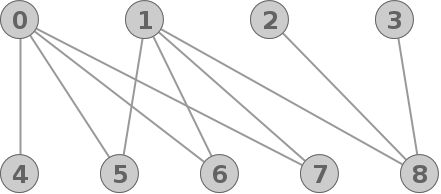
\includegraphics[scale = 0.2]{img/ej3/busqueda_local/k5,4Nocompleto_st0.png} &
			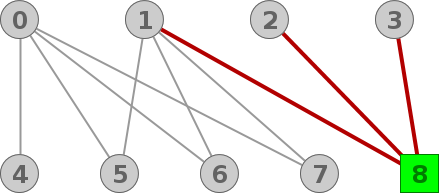
\includegraphics[scale = 0.2]{img/ej3/busqueda_local/k5,4Nocompleto_st1.png} & 
			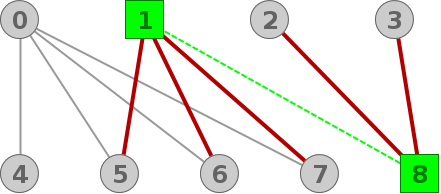
\includegraphics[scale = 0.2]{img/ej3/busqueda_local/k5,4Nocompleto_st2.png} \\
		\hline
		\end{tabular}
	\end{center}
\end{figure}
En este caso el grado promedio es $2,2$ con lo que podr\'ia suceder 
(con las etiquetas correctas) que la busqueda local comience con el
nodo marcado como $8$ en el ejemplo, cosa que en la golosa 
constructiva no pod\'ia suceder.

Para los \'arboles tambi\'en analizaremos el caso extremo presentado 
en la figura \ref{fig:extremo_arboles} y analizaremos nuevamente
la curiosidad de que debido a la relajaci\'on en el criterio de 
selecci\'on del primer nodo en busqueda local, existe una 
construccion alternativa de la clique devuelta por la heur\'istica
aunque sobre este ejemplo la respuesta ser\'a sub-optima.

\begin{figure}[H]
\caption{Resultado sub-\'optimo del ejemplo extremo para \'arboles - 
Forma alternativa}
\begin{center}
		\begin{tabular}{|c||c||c|}
		\hline
		Grafo de entrada & Paso 1 & Paso 2 \\ 
			\hline
			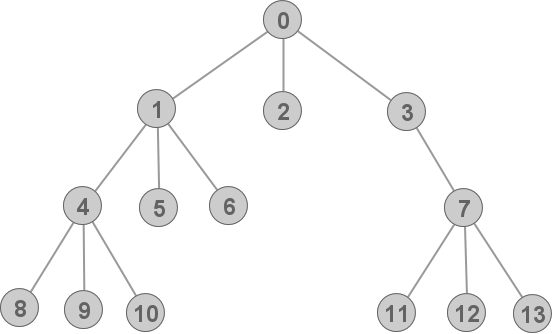
\includegraphics[scale = 0.2]{img/ej3/busqueda_local/extremetree_st0.png} &
			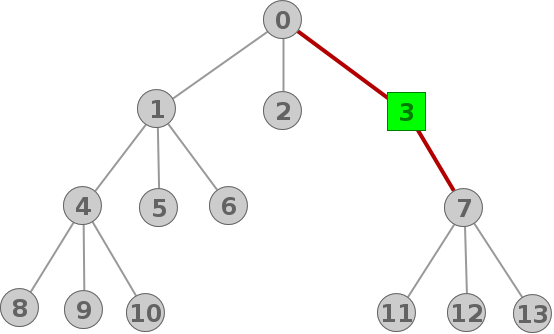
\includegraphics[scale = 0.2]{img/ej3/busqueda_local/extremetree_st11.png} & 
			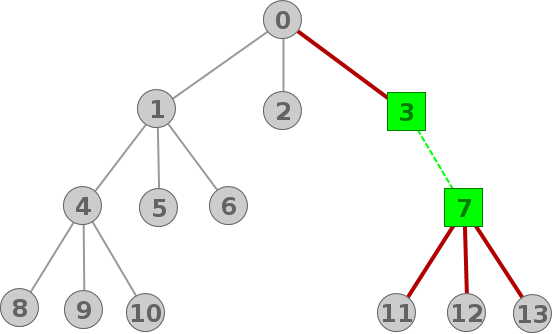
\includegraphics[scale = 0.2]{img/ej3/busqueda_local/extremetree_st12.png} \\
		\hline
		\end{tabular}
	\end{center}
\end{figure}
Notar que aqu\'i el grado promedio es aproximadamente $1,8$ con lo que 
el nodo identificado como $3$ en el ejemplo es elegible como
primer nodo de $K$ pues $2 > 1,8$.

\subsubsection{Estrella + Puente + CMF}

En esta familia, siguiendo con la idea de las \'ultimas dos analizadas
podemos ver que que para llegar a la soluci\'on \'optima hay muchos 
m\'as puntos de inicio que en la golosa constructiva. Por ejemplo
el primer nodo puede estar en $K_{\Delta -1}$ y no ser siquiera $v'$ 
(ver Figura \ref{fig:epcmf_carac}), en los casos en los que esto 
suceda, en la variante b\'asica, la busqueda local elegir\'a
$\left\lfloor \frac{\Delta -1}{2} \right\rfloor$ nodos de $K_{\Delta -1}$. 
Si estos nodos incluyen a $v'$, termina pues no quedan candidatos que
hagan crecer la soluci\'on parcial, si no lo incluyen hay dos posibilidades:

\begin{itemize}
	\item $\Delta$ par: La cantidad de nodos en $K_{\Delta -1}$ ser\'a impar 
	y entonces la soluci\'on crece hasta alcanzar
	$\left\lfloor \frac{\Delta -1}{2} \right\rfloor$ nodos que por hip\'otesis
	no incluyen a $v'$, en el siguiente paso el \'unico candidato restante
	que hace crecer la soluci\'on en una arista es $v'$ y por ello lo agrega 
	a la soluci\'on, terminando con una soluci\'on \'optima.
	\begin{center}
	\begin{tabular}{|c||c|}
		\hline
		Grafo entrada & 
		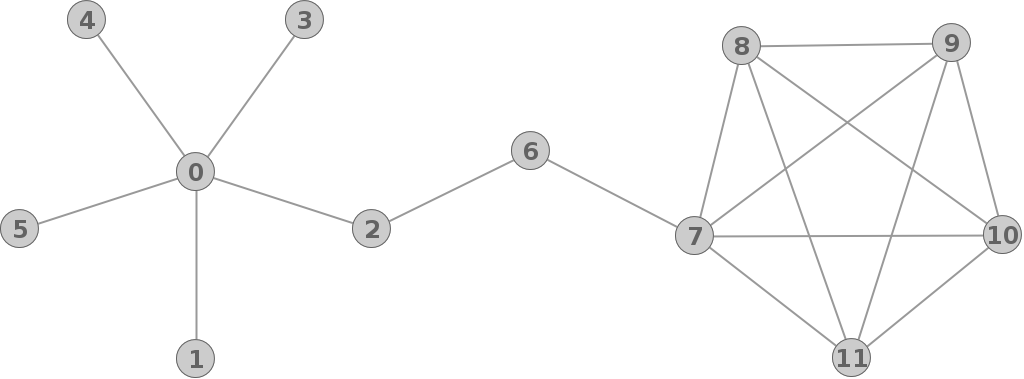
\includegraphics[scale = 0.2]{img/ej3/busqueda_local/estrellaPuenteCMFImpar.png} \\
		\hline
		Primer paso &
		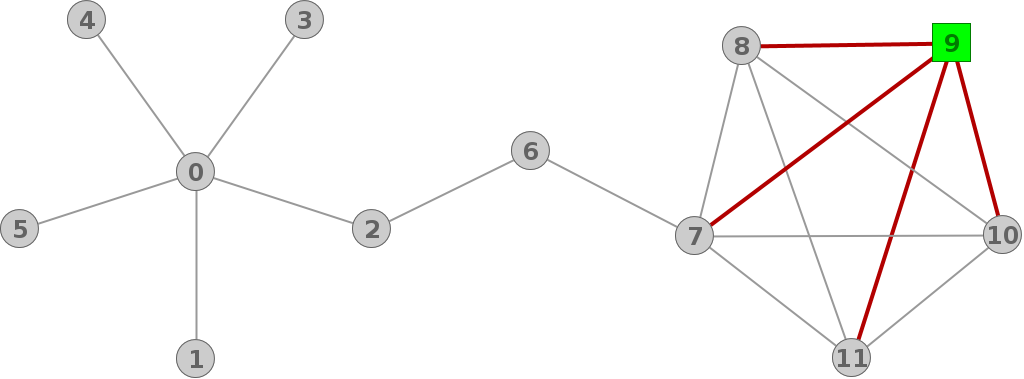
\includegraphics[scale = 0.2]{img/ej3/busqueda_local/estrellaPuenteCMFImpar_st01.png} \\
		\hline
		Segundo paso &
		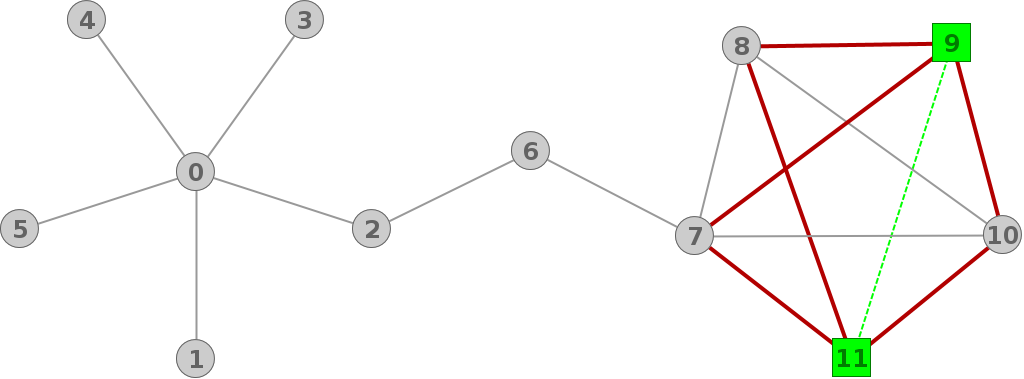
\includegraphics[scale = 0.2]{img/ej3/busqueda_local/estrellaPuenteCMFImpar_st02.png} \\
		\hline
		Tercer paso &
		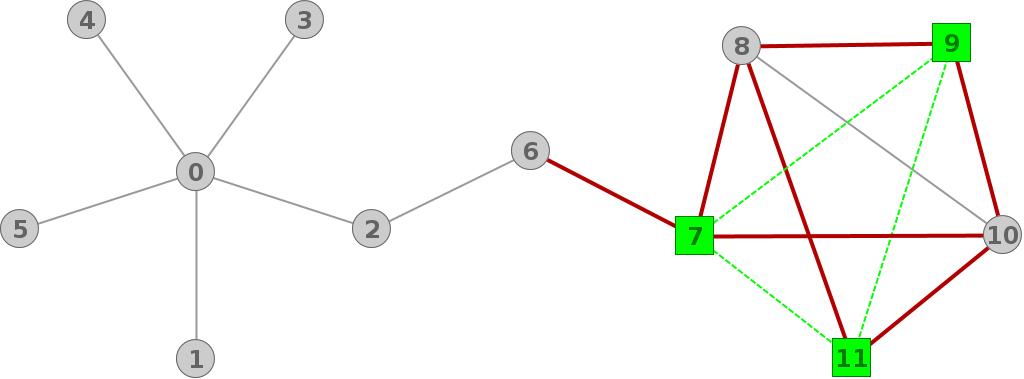
\includegraphics[scale = 0.2]{img/ej3/busqueda_local/estrellaPuenteCMFImpar_st03.png} \\
		\hline

	\end{tabular}
	\end{center}


	\item $\Delta$ impar: La cantidad de nodos en $K_{\Delta -1}$ ser\'a par, 
	en este caso la soluci\'on crece hasta alcanzar $\frac{\Delta -1}{2}$ nodos
	que no incluyen a $v'$, llegados a este punto la soluci\'on no puede crecer
	para incluir a $v'$ ya que de hacerlo la frontera de la soluci\'on ser\'ia
	la misma que en el paso anterior y el algoritmo no se comporta de esta manera.
	Por ende la soluci\'on devuelta es sub-\'optima.
	\begin{center}
	\begin{tabular}{|c||c|}
		\hline
		Grafo entrada & 
		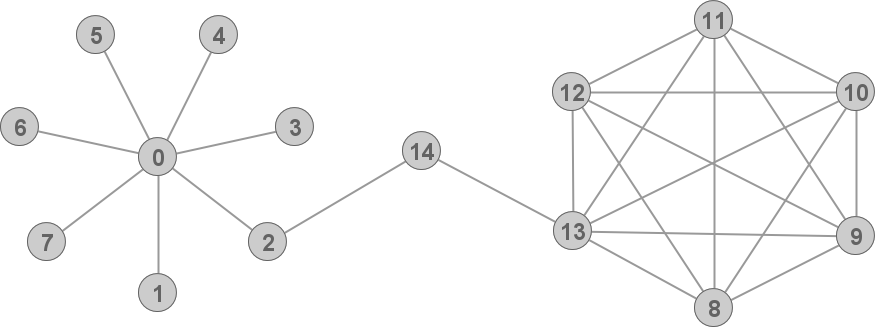
\includegraphics[scale = 0.2]{img/ej3/busqueda_local/estrellaPuenteCMFPar.png} \\
		\hline
		Primer paso &
		\includegraphics[scale = 0.2]{img/ej3/busqueda_local/estrellaPuenteCMFPar_st01.png} \\
		\hline
		Segundo paso &
		\includegraphics[scale = 0.2]{img/ej3/busqueda_local/estrellaPuenteCMFPar_st02.png} \\
		\hline
		Tercer paso &
		\includegraphics[scale = 0.2]{img/ej3/busqueda_local/estrellaPuenteCMFPar_st03.png} \\
		\hline

	\end{tabular}
	\end{center}


\end{itemize}

Notar que en la variante \emph{Mejor Vecino} evita el resultado sub-\'optimo en 
el \'ultimo caso (bajo las hip\'otesis del mismo).

Hay otros posibles comportamientos de la heur\'istica sobre la misma familia de
grafos, que el algoritmo comience la soluci\'on en uno de los nodos del puente o
que la comience en el centro de la estrella.

Que comience la soluci\'on sobre el puente es un caso que t\'ipicamente no va a 
suceder, si es un puente simple (camino simple) la \'unica forma de que sucediera
ser\'ia si el puente es lo suficientemente largo para bajar el grado promedio a
un valor menor a dos, si el puente no es un camino simple y en cambio tiene nodos
extra, el puente no tendr\'a que ser tan largo pero siempre se deber\'a cumplir
que el nodo inicial de la soluci\'on tenga grado mayor al grado promedio del grafo.

Cuando la soluci\'on se inicia en el centro de la estrella, la busqueda local 
se estanca en el m\'aximo local debido al puente que une la estrella con $K_{\Delta -1}$,
de hecho, esta familia fue dise\~nada con el objetivo de asegurar precisamente
este estancamiento.
		



\subsection{Experimentaci\'on}
    \subsubsection{Resultados}
\par Se presentan a continuaci\'on los resultados de la experimentaci\'on
    de la heur\'istica golosa constructiva para \emph{CMF}. La experimentaci\'on se realiz\'o
    con las instancias ya generadas (seg\'un se explica en \emph{\nameref{notas_preliminares},
    \nameref{notas:datasets}} y \emph{\nameref{notas:experimentacion}}).

\par Para recordar, se cuentan con 10 instancias aleatorias de cada tama\~no,
    las cuales fueron resueltas 5 veces cada una y nos quedamos con el menor tiempo
    requerido de esas 5 ejecuciones. Por \'ultimo, tomamos el promedio de este tiempo
    requerido calculado entre las instancias del mismo tama\~no (10, como se ha
    dicho).

\bigskip

\begin{figure}[H]
    \centering
    \fontsize{8}{10}\selectfont
    \resizebox{0.8\textwidth}{!}{% GNUPLOT: LaTeX picture with Postscript
\begingroup
  \makeatletter
  \providecommand\color[2][]{%
    \GenericError{(gnuplot) \space\space\space\@spaces}{%
      Package color not loaded in conjunction with
      terminal option `colourtext'%
    }{See the gnuplot documentation for explanation.%
    }{Either use 'blacktext' in gnuplot or load the package
      color.sty in LaTeX.}%
    \renewcommand\color[2][]{}%
  }%
  \providecommand\includegraphics[2][]{%
    \GenericError{(gnuplot) \space\space\space\@spaces}{%
      Package graphicx or graphics not loaded%
    }{See the gnuplot documentation for explanation.%
    }{The gnuplot epslatex terminal needs graphicx.sty or graphics.sty.}%
    \renewcommand\includegraphics[2][]{}%
  }%
  \providecommand\rotatebox[2]{#2}%
  \@ifundefined{ifGPcolor}{%
    \newif\ifGPcolor
    \GPcolortrue
  }{}%
  \@ifundefined{ifGPblacktext}{%
    \newif\ifGPblacktext
    \GPblacktexttrue
  }{}%
  % define a \g@addto@macro without @ in the name:
  \let\gplgaddtomacro\g@addto@macro
  % define empty templates for all commands taking text:
  \gdef\gplbacktext{}%
  \gdef\gplfronttext{}%
  \makeatother
  \ifGPblacktext
    % no textcolor at all
    \def\colorrgb#1{}%
    \def\colorgray#1{}%
  \else
    % gray or color?
    \ifGPcolor
      \def\colorrgb#1{\color[rgb]{#1}}%
      \def\colorgray#1{\color[gray]{#1}}%
      \expandafter\def\csname LTw\endcsname{\color{white}}%
      \expandafter\def\csname LTb\endcsname{\color{black}}%
      \expandafter\def\csname LTa\endcsname{\color{black}}%
      \expandafter\def\csname LT0\endcsname{\color[rgb]{1,0,0}}%
      \expandafter\def\csname LT1\endcsname{\color[rgb]{0,1,0}}%
      \expandafter\def\csname LT2\endcsname{\color[rgb]{0,0,1}}%
      \expandafter\def\csname LT3\endcsname{\color[rgb]{1,0,1}}%
      \expandafter\def\csname LT4\endcsname{\color[rgb]{0,1,1}}%
      \expandafter\def\csname LT5\endcsname{\color[rgb]{1,1,0}}%
      \expandafter\def\csname LT6\endcsname{\color[rgb]{0,0,0}}%
      \expandafter\def\csname LT7\endcsname{\color[rgb]{1,0.3,0}}%
      \expandafter\def\csname LT8\endcsname{\color[rgb]{0.5,0.5,0.5}}%
    \else
      % gray
      \def\colorrgb#1{\color{black}}%
      \def\colorgray#1{\color[gray]{#1}}%
      \expandafter\def\csname LTw\endcsname{\color{white}}%
      \expandafter\def\csname LTb\endcsname{\color{black}}%
      \expandafter\def\csname LTa\endcsname{\color{black}}%
      \expandafter\def\csname LT0\endcsname{\color{black}}%
      \expandafter\def\csname LT1\endcsname{\color{black}}%
      \expandafter\def\csname LT2\endcsname{\color{black}}%
      \expandafter\def\csname LT3\endcsname{\color{black}}%
      \expandafter\def\csname LT4\endcsname{\color{black}}%
      \expandafter\def\csname LT5\endcsname{\color{black}}%
      \expandafter\def\csname LT6\endcsname{\color{black}}%
      \expandafter\def\csname LT7\endcsname{\color{black}}%
      \expandafter\def\csname LT8\endcsname{\color{black}}%
    \fi
  \fi
  \setlength{\unitlength}{0.0500bp}%
  \begin{picture}(7200.00,5040.00)%
    \gplgaddtomacro\gplbacktext{%
      \csname LTb\endcsname%
      \put(1430,2244){\makebox(0,0)[r]{\strut{} 0}}%
      \csname LTb\endcsname%
      \put(1430,2549){\makebox(0,0)[r]{\strut{} 5000}}%
      \csname LTb\endcsname%
      \put(1430,2854){\makebox(0,0)[r]{\strut{} 10000}}%
      \csname LTb\endcsname%
      \put(1430,3159){\makebox(0,0)[r]{\strut{} 15000}}%
      \csname LTb\endcsname%
      \put(1430,3464){\makebox(0,0)[r]{\strut{} 20000}}%
      \csname LTb\endcsname%
      \put(1430,3769){\makebox(0,0)[r]{\strut{} 25000}}%
      \csname LTb\endcsname%
      \put(1430,4074){\makebox(0,0)[r]{\strut{} 30000}}%
      \csname LTb\endcsname%
      \put(1430,4379){\makebox(0,0)[r]{\strut{} 35000}}%
      \csname LTb\endcsname%
      \put(1562,2024){\makebox(0,0){\strut{} 0}}%
      \csname LTb\endcsname%
      \put(2086,2024){\makebox(0,0){\strut{} 500}}%
      \csname LTb\endcsname%
      \put(2610,2024){\makebox(0,0){\strut{} 1000}}%
      \csname LTb\endcsname%
      \put(3134,2024){\makebox(0,0){\strut{} 1500}}%
      \csname LTb\endcsname%
      \put(3658,2024){\makebox(0,0){\strut{} 2000}}%
      \csname LTb\endcsname%
      \put(4183,2024){\makebox(0,0){\strut{} 2500}}%
      \csname LTb\endcsname%
      \put(4707,2024){\makebox(0,0){\strut{} 3000}}%
      \csname LTb\endcsname%
      \put(5231,2024){\makebox(0,0){\strut{} 3500}}%
      \csname LTb\endcsname%
      \put(5755,2024){\makebox(0,0){\strut{} 4000}}%
      \csname LTb\endcsname%
      \put(6279,2024){\makebox(0,0){\strut{} 4500}}%
      \csname LTb\endcsname%
      \put(6803,2024){\makebox(0,0){\strut{} 5000}}%
      \put(176,3311){\rotatebox{-270}{\makebox(0,0){\strut{}Tiempo (nanosegundos)}}}%
      \put(396,3311){\rotatebox{-270}{\makebox(0,0){\strut{}(Escala Lineal)}}}%
      \put(4182,1694){\makebox(0,0){\strut{}Cantidad de Nodos}}%
      \put(4182,1474){\makebox(0,0){\strut{}(Escala Lineal)}}%
      \put(4182,4709){\makebox(0,0){\strut{}Tiempo de ejecución conforme aumenta la cantidad de nodos}}%
    }%
    \gplgaddtomacro\gplfronttext{%
      \csname LTb\endcsname%
      \put(5735,1053){\makebox(0,0)[r]{\strut{}Grafos Completos}}%
      \csname LTb\endcsname%
      \put(5735,833){\makebox(0,0)[r]{\strut{}Arboles}}%
      \csname LTb\endcsname%
      \put(5735,613){\makebox(0,0)[r]{\strut{}Circulares}}%
      \csname LTb\endcsname%
      \put(5735,393){\makebox(0,0)[r]{\strut{}Cota teórica superior $\mathcal O(n^2)$}}%
      \csname LTb\endcsname%
      \put(5735,173){\makebox(0,0)[r]{\strut{}Cota teórica superior $\mathcal O(n)$}}%
    }%
    \gplbacktext
    \put(0,0){\includegraphics{ej3_nodos_completos_arboles_circulares}}%
    \gplfronttext
  \end{picture}%
\endgroup
}
    \caption{Complejidad temporal para grafos completos, \'arboles y circulares}
\end{figure}

\begin{figure}[H]
    \centering
    \fontsize{8}{10}\selectfont
    \resizebox{0.8\textwidth}{!}{% GNUPLOT: LaTeX picture with Postscript
\begingroup
  \makeatletter
  \providecommand\color[2][]{%
    \GenericError{(gnuplot) \space\space\space\@spaces}{%
      Package color not loaded in conjunction with
      terminal option `colourtext'%
    }{See the gnuplot documentation for explanation.%
    }{Either use 'blacktext' in gnuplot or load the package
      color.sty in LaTeX.}%
    \renewcommand\color[2][]{}%
  }%
  \providecommand\includegraphics[2][]{%
    \GenericError{(gnuplot) \space\space\space\@spaces}{%
      Package graphicx or graphics not loaded%
    }{See the gnuplot documentation for explanation.%
    }{The gnuplot epslatex terminal needs graphicx.sty or graphics.sty.}%
    \renewcommand\includegraphics[2][]{}%
  }%
  \providecommand\rotatebox[2]{#2}%
  \@ifundefined{ifGPcolor}{%
    \newif\ifGPcolor
    \GPcolortrue
  }{}%
  \@ifundefined{ifGPblacktext}{%
    \newif\ifGPblacktext
    \GPblacktexttrue
  }{}%
  % define a \g@addto@macro without @ in the name:
  \let\gplgaddtomacro\g@addto@macro
  % define empty templates for all commands taking text:
  \gdef\gplbacktext{}%
  \gdef\gplfronttext{}%
  \makeatother
  \ifGPblacktext
    % no textcolor at all
    \def\colorrgb#1{}%
    \def\colorgray#1{}%
  \else
    % gray or color?
    \ifGPcolor
      \def\colorrgb#1{\color[rgb]{#1}}%
      \def\colorgray#1{\color[gray]{#1}}%
      \expandafter\def\csname LTw\endcsname{\color{white}}%
      \expandafter\def\csname LTb\endcsname{\color{black}}%
      \expandafter\def\csname LTa\endcsname{\color{black}}%
      \expandafter\def\csname LT0\endcsname{\color[rgb]{1,0,0}}%
      \expandafter\def\csname LT1\endcsname{\color[rgb]{0,1,0}}%
      \expandafter\def\csname LT2\endcsname{\color[rgb]{0,0,1}}%
      \expandafter\def\csname LT3\endcsname{\color[rgb]{1,0,1}}%
      \expandafter\def\csname LT4\endcsname{\color[rgb]{0,1,1}}%
      \expandafter\def\csname LT5\endcsname{\color[rgb]{1,1,0}}%
      \expandafter\def\csname LT6\endcsname{\color[rgb]{0,0,0}}%
      \expandafter\def\csname LT7\endcsname{\color[rgb]{1,0.3,0}}%
      \expandafter\def\csname LT8\endcsname{\color[rgb]{0.5,0.5,0.5}}%
    \else
      % gray
      \def\colorrgb#1{\color{black}}%
      \def\colorgray#1{\color[gray]{#1}}%
      \expandafter\def\csname LTw\endcsname{\color{white}}%
      \expandafter\def\csname LTb\endcsname{\color{black}}%
      \expandafter\def\csname LTa\endcsname{\color{black}}%
      \expandafter\def\csname LT0\endcsname{\color{black}}%
      \expandafter\def\csname LT1\endcsname{\color{black}}%
      \expandafter\def\csname LT2\endcsname{\color{black}}%
      \expandafter\def\csname LT3\endcsname{\color{black}}%
      \expandafter\def\csname LT4\endcsname{\color{black}}%
      \expandafter\def\csname LT5\endcsname{\color{black}}%
      \expandafter\def\csname LT6\endcsname{\color{black}}%
      \expandafter\def\csname LT7\endcsname{\color{black}}%
      \expandafter\def\csname LT8\endcsname{\color{black}}%
    \fi
  \fi
  \setlength{\unitlength}{0.0500bp}%
  \begin{picture}(7200.00,5040.00)%
    \gplgaddtomacro\gplbacktext{%
      \csname LTb\endcsname%
      \put(1166,2244){\makebox(0,0)[r]{\strut{} 0}}%
      \csname LTb\endcsname%
      \put(1166,2511){\makebox(0,0)[r]{\strut{} 100}}%
      \csname LTb\endcsname%
      \put(1166,2778){\makebox(0,0)[r]{\strut{} 200}}%
      \csname LTb\endcsname%
      \put(1166,3045){\makebox(0,0)[r]{\strut{} 300}}%
      \csname LTb\endcsname%
      \put(1166,3312){\makebox(0,0)[r]{\strut{} 400}}%
      \csname LTb\endcsname%
      \put(1166,3578){\makebox(0,0)[r]{\strut{} 500}}%
      \csname LTb\endcsname%
      \put(1166,3845){\makebox(0,0)[r]{\strut{} 600}}%
      \csname LTb\endcsname%
      \put(1166,4112){\makebox(0,0)[r]{\strut{} 700}}%
      \csname LTb\endcsname%
      \put(1166,4379){\makebox(0,0)[r]{\strut{} 800}}%
      \csname LTb\endcsname%
      \put(1298,2024){\makebox(0,0){\strut{} 0}}%
      \csname LTb\endcsname%
      \put(1849,2024){\makebox(0,0){\strut{} 500}}%
      \csname LTb\endcsname%
      \put(2399,2024){\makebox(0,0){\strut{} 1000}}%
      \csname LTb\endcsname%
      \put(2950,2024){\makebox(0,0){\strut{} 1500}}%
      \csname LTb\endcsname%
      \put(3500,2024){\makebox(0,0){\strut{} 2000}}%
      \csname LTb\endcsname%
      \put(4051,2024){\makebox(0,0){\strut{} 2500}}%
      \csname LTb\endcsname%
      \put(4601,2024){\makebox(0,0){\strut{} 3000}}%
      \csname LTb\endcsname%
      \put(5152,2024){\makebox(0,0){\strut{} 3500}}%
      \csname LTb\endcsname%
      \put(5702,2024){\makebox(0,0){\strut{} 4000}}%
      \csname LTb\endcsname%
      \put(6253,2024){\makebox(0,0){\strut{} 4500}}%
      \csname LTb\endcsname%
      \put(6803,2024){\makebox(0,0){\strut{} 5000}}%
      \put(176,3311){\rotatebox{-270}{\makebox(0,0){\strut{}Tiempo (microsegundos)}}}%
      \put(396,3311){\rotatebox{-270}{\makebox(0,0){\strut{}(Escala Lineal)}}}%
      \put(4050,1694){\makebox(0,0){\strut{}Cantidad de Nodos}}%
      \put(4050,1474){\makebox(0,0){\strut{}(Escala Lineal)}}%
      \put(4050,4709){\makebox(0,0){\strut{}Tiempo de ejecución conforme aumenta la cantidad de nodos}}%
    }%
    \gplgaddtomacro\gplfronttext{%
      \csname LTb\endcsname%
      \put(5603,1053){\makebox(0,0)[r]{\strut{}Estrellas}}%
      \csname LTb\endcsname%
      \put(5603,833){\makebox(0,0)[r]{\strut{}Ruedas}}%
      \csname LTb\endcsname%
      \put(5603,613){\makebox(0,0)[r]{\strut{}Banana Tree}}%
      \csname LTb\endcsname%
      \put(5603,393){\makebox(0,0)[r]{\strut{}Bipartitos}}%
      \csname LTb\endcsname%
      \put(5603,173){\makebox(0,0)[r]{\strut{}Cota teórica superior $\mathcal O(n^2)$}}%
    }%
    \gplbacktext
    \put(0,0){\includegraphics{ej3_nodos_estrella_rueda_banana_bipartito}}%
    \gplfronttext
  \end{picture}%
\endgroup
}
    \caption{Complejidad temporal para grafos estrella, rueda, banana tree y bipartitos}
\end{figure}

\begin{figure}[H]
    \centering
    \fontsize{8}{10}\selectfont
    \resizebox{0.8\textwidth}{!}{% GNUPLOT: LaTeX picture with Postscript
\begingroup
  \makeatletter
  \providecommand\color[2][]{%
    \GenericError{(gnuplot) \space\space\space\@spaces}{%
      Package color not loaded in conjunction with
      terminal option `colourtext'%
    }{See the gnuplot documentation for explanation.%
    }{Either use 'blacktext' in gnuplot or load the package
      color.sty in LaTeX.}%
    \renewcommand\color[2][]{}%
  }%
  \providecommand\includegraphics[2][]{%
    \GenericError{(gnuplot) \space\space\space\@spaces}{%
      Package graphicx or graphics not loaded%
    }{See the gnuplot documentation for explanation.%
    }{The gnuplot epslatex terminal needs graphicx.sty or graphics.sty.}%
    \renewcommand\includegraphics[2][]{}%
  }%
  \providecommand\rotatebox[2]{#2}%
  \@ifundefined{ifGPcolor}{%
    \newif\ifGPcolor
    \GPcolortrue
  }{}%
  \@ifundefined{ifGPblacktext}{%
    \newif\ifGPblacktext
    \GPblacktexttrue
  }{}%
  % define a \g@addto@macro without @ in the name:
  \let\gplgaddtomacro\g@addto@macro
  % define empty templates for all commands taking text:
  \gdef\gplbacktext{}%
  \gdef\gplfronttext{}%
  \makeatother
  \ifGPblacktext
    % no textcolor at all
    \def\colorrgb#1{}%
    \def\colorgray#1{}%
  \else
    % gray or color?
    \ifGPcolor
      \def\colorrgb#1{\color[rgb]{#1}}%
      \def\colorgray#1{\color[gray]{#1}}%
      \expandafter\def\csname LTw\endcsname{\color{white}}%
      \expandafter\def\csname LTb\endcsname{\color{black}}%
      \expandafter\def\csname LTa\endcsname{\color{black}}%
      \expandafter\def\csname LT0\endcsname{\color[rgb]{1,0,0}}%
      \expandafter\def\csname LT1\endcsname{\color[rgb]{0,1,0}}%
      \expandafter\def\csname LT2\endcsname{\color[rgb]{0,0,1}}%
      \expandafter\def\csname LT3\endcsname{\color[rgb]{1,0,1}}%
      \expandafter\def\csname LT4\endcsname{\color[rgb]{0,1,1}}%
      \expandafter\def\csname LT5\endcsname{\color[rgb]{1,1,0}}%
      \expandafter\def\csname LT6\endcsname{\color[rgb]{0,0,0}}%
      \expandafter\def\csname LT7\endcsname{\color[rgb]{1,0.3,0}}%
      \expandafter\def\csname LT8\endcsname{\color[rgb]{0.5,0.5,0.5}}%
    \else
      % gray
      \def\colorrgb#1{\color{black}}%
      \def\colorgray#1{\color[gray]{#1}}%
      \expandafter\def\csname LTw\endcsname{\color{white}}%
      \expandafter\def\csname LTb\endcsname{\color{black}}%
      \expandafter\def\csname LTa\endcsname{\color{black}}%
      \expandafter\def\csname LT0\endcsname{\color{black}}%
      \expandafter\def\csname LT1\endcsname{\color{black}}%
      \expandafter\def\csname LT2\endcsname{\color{black}}%
      \expandafter\def\csname LT3\endcsname{\color{black}}%
      \expandafter\def\csname LT4\endcsname{\color{black}}%
      \expandafter\def\csname LT5\endcsname{\color{black}}%
      \expandafter\def\csname LT6\endcsname{\color{black}}%
      \expandafter\def\csname LT7\endcsname{\color{black}}%
      \expandafter\def\csname LT8\endcsname{\color{black}}%
    \fi
  \fi
  \setlength{\unitlength}{0.0500bp}%
  \begin{picture}(7200.00,5040.00)%
    \gplgaddtomacro\gplbacktext{%
      \csname LTb\endcsname%
      \put(1166,1804){\makebox(0,0)[r]{\strut{} 0}}%
      \csname LTb\endcsname%
      \put(1166,2090){\makebox(0,0)[r]{\strut{} 50}}%
      \csname LTb\endcsname%
      \put(1166,2376){\makebox(0,0)[r]{\strut{} 100}}%
      \csname LTb\endcsname%
      \put(1166,2662){\makebox(0,0)[r]{\strut{} 150}}%
      \csname LTb\endcsname%
      \put(1166,2948){\makebox(0,0)[r]{\strut{} 200}}%
      \csname LTb\endcsname%
      \put(1166,3235){\makebox(0,0)[r]{\strut{} 250}}%
      \csname LTb\endcsname%
      \put(1166,3521){\makebox(0,0)[r]{\strut{} 300}}%
      \csname LTb\endcsname%
      \put(1166,3807){\makebox(0,0)[r]{\strut{} 350}}%
      \csname LTb\endcsname%
      \put(1166,4093){\makebox(0,0)[r]{\strut{} 400}}%
      \csname LTb\endcsname%
      \put(1166,4379){\makebox(0,0)[r]{\strut{} 450}}%
      \csname LTb\endcsname%
      \put(1298,1584){\makebox(0,0){\strut{} 0}}%
      \csname LTb\endcsname%
      \put(1849,1584){\makebox(0,0){\strut{} 500}}%
      \csname LTb\endcsname%
      \put(2399,1584){\makebox(0,0){\strut{} 1000}}%
      \csname LTb\endcsname%
      \put(2950,1584){\makebox(0,0){\strut{} 1500}}%
      \csname LTb\endcsname%
      \put(3500,1584){\makebox(0,0){\strut{} 2000}}%
      \csname LTb\endcsname%
      \put(4051,1584){\makebox(0,0){\strut{} 2500}}%
      \csname LTb\endcsname%
      \put(4601,1584){\makebox(0,0){\strut{} 3000}}%
      \csname LTb\endcsname%
      \put(5152,1584){\makebox(0,0){\strut{} 3500}}%
      \csname LTb\endcsname%
      \put(5702,1584){\makebox(0,0){\strut{} 4000}}%
      \csname LTb\endcsname%
      \put(6253,1584){\makebox(0,0){\strut{} 4500}}%
      \csname LTb\endcsname%
      \put(6803,1584){\makebox(0,0){\strut{} 5000}}%
      \put(176,3091){\rotatebox{-270}{\makebox(0,0){\strut{}Tiempo (microsegundos)}}}%
      \put(396,3091){\rotatebox{-270}{\makebox(0,0){\strut{}(Escala Lineal)}}}%
      \put(4050,1254){\makebox(0,0){\strut{}Cantidad de Nodos}}%
      \put(4050,1034){\makebox(0,0){\strut{}(Escala Lineal)}}%
      \put(4050,4709){\makebox(0,0){\strut{}Tiempo de ejecución conforme aumenta la cantidad de nodos}}%
    }%
    \gplgaddtomacro\gplfronttext{%
      \csname LTb\endcsname%
      \put(5603,613){\makebox(0,0)[r]{\strut{}Estrella+CMF}}%
      \csname LTb\endcsname%
      \put(5603,393){\makebox(0,0)[r]{\strut{}Estrella+Puente+CMF}}%
      \csname LTb\endcsname%
      \put(5603,173){\makebox(0,0)[r]{\strut{}Cota teórica superior $\mathcal O(n^2)$}}%
    }%
    \gplbacktext
    \put(0,0){\includegraphics{ej3_nodos_disruptivas}}%
    \gplfronttext
  \end{picture}%
\endgroup
}
    \caption{Complejidad temporal para grafos Estrella+CMF, Estrella+Puente+CMF}
\end{figure}

\subsubsection{Conclusiones}
\par En los primeros 2 resultados se puede observar que la complejidad asint\'otica
    para las familias ``simples''\footnote{Consideramos a los grafos completos
    como una familia simple pues con los datos de entrada resolver el problema
    de \emph{CMF} es trivial.} (pocas aristas y con estructuras muy restrictivas)
    es similar. Si bien hay diferencias (en el orden de los nanosegundos), se
    destaca que todas cumplen con la complejidad asint\'otica temporal te\'orica
    calculada y a su vez se comportan de la misma manera en cuanto a crecimiento.

\par En el segundo gr\'afico, tambi\'en se cuentan con una serie de familias
    ``simples'', pero aqu\'i el comportamiento de nuestra heur\'istica resulta
    un tanto m\'as err\'atico, si bien sigue estando en el orden de complejidad
    calculado. Se puede observar que mientras que las familias de las 
    Rueadas y las estrellas (de estructuras muy similares) se comportan pr\'acticamente
    igual, para los grafos bipartitos se requiere menor tiempo para resolver
    instancias del mismo tama\~no. Esto es un tanto raro, ya que en las 3 familias
    (como ya se ha explicado) la \emph{CMF} tendr\'a el mismo tama\~no. S\'olo
    nos queda hipotetizar\footnote{Viernes 22 de Noviembre, 17:58 hs GMT-3} sobre los motivos.

\par En el caso de la familia de grafos \emph{Banana Tree}, suponemos que su comportamiento
    se debe que seg\'un el tama\~no de las estrellas que tenga en sus extremos, el nodo
    de mayor grado estar\'a en alguna estrella o en el nodo central que une a todas las estrellas.
    Este dato tendr\'a una influencia inmediata en la elecci\'on de los nodos candidatos
    a agregarse a la clique luego de haber encontrado el nodo de mayor grado del grafo (ya
    que si las estrellas/extremidades son de tama\~no considerable, las mismas
    deberan ser tenidas en cuenta, mientras que si solo se tiene una gran estrella (las
    ``bananas'' son de taman\~o 1), esto ser\'a m\'as eficiente.

\par Por \'ultimo, observamos que el comportamiento para las familias Estrella+CMF y
    Estrella+Puente+CMF es muy estable a medida que crece el taman\~o de las instancias.
    Quiz\'as lo m\'as interesantes de estas familias (aparte de comprobar que cumplen
    con la complejidad asint\'otica te\'orica) es comparar los resultados otorgados
    por la heur\'istica con el algoritmo exacto u las dem\'as heur\'isticas. Esto
    se efectua en la Secci\'on~\ref{experimentacion} de este trabajo.


        \pagebreak

    \section{Metaheur\'istica de B\'usqueda Tab\'u}
        \subsection{Resoluci\'on}
    \begin{algorithm}[H]
    \caption{Heur\'istica Golosa Constructiva 1 para \emph{CMF} - Descriptivo}
    \begin{algorithmic}[1]
        \Require\Statex
            \begin{itemize}
                \item Un grafo $G$ de $n$ v\'ertices y $m$ aristas.

                \item Una funci\'on $candidatos(K)$, que dado un conjunto de v\'ertices
                    $K$, devuelve el conjunto de v\'ertices de $G$ que son adjacentes
                    a todos los elementos de $K$, cuyo grado es mayor $2|K|$.
            \end{itemize}

        \Statex

        \Ensure Una \emph{clique} $K$ de $G$ con una frontera $\delta(K)$ que se
            espera que sea de cardinalidad cercana o igual a la de $\delta(K')$,
            siendo $K'$ la \emph{clique} de m\'axima frontera de $G$.

        \Statex

        \State Sea $v$ el v\'ertice de mayor grado en $G$.
        \State $K \gets \{v\}$
        \While{$candidatos(K) \neq \emptyset$}
            \State Sea $v'$ el v\'ertice de mayor grado en $candidatos(K)$.
            \State $K \gets K \cup \{v'\}$
        \EndWhile

        \State \Return{$K$}
    \end{algorithmic}
\end{algorithm}

\begin{algorithm}[H]
    \caption{Heur\'istica Golosa Constructiva 2 para \emph{CMF} - Descriptivo}
    \begin{algorithmic}[1]
        \Require Un grafo $G$ de $n$ v\'ertices y $m$ aristas.
        \Ensure Una \emph{clique} $K$ de $G$ con una frontera $\delta(K)$ que se
            espera que sea de cardinalidad cercana o igual a la de $\delta(K')$,
            siendo $K'$ la \emph{clique} de m\'axima frontera de $G$.

        \Statex

        \State $K \gets \emptyset$
        \State $\delta_{max} \gets 0$
        \State $Ks \gets $ Todos los conjuntos de 2 o 3 v\'ertices de $G$ que
            forman una \emph{clique}.
        \ForEach{$K' \in Ks$}
            \If{$\delta(K') > \delta_{max}$}
                \State $\delta_{max} \gets \delta(K')$
                \State $K \gets K'$

            \EndIf

        \EndForEach

        \State \Return{$K$}
    \end{algorithmic}
\end{algorithm}


\subsection{Complejidad}
    \subsubsection{Estructuras de Datos}

\subsubsection{Pseudoc\'odigo de complejidad}
\par Se presenta a continuaci\'on un pseudoc\'odigo m\'as espec\'ifico de la implementaci\'on
    de este algoritmo provista junto con este trabajo. El mismo tiene en cuenta
    las estructuras de datos explicadas en el punto anterior.

\par Luego del pseudoc\'odigo se justifican detalladamente las complejidades
    expuestas a continuaci\'on que no sean evidentes\footnote{Consideramos
    como "complejidades evidentes" las asignaciones de variables, operaciones
    m\'atematicas simples, asignaciones/inicializaci\'on de posiciones de
    un vector/\emph{deque} o cualquier contenedor de acceso aleatorio/arbitrario}.

\bigskip

\begin{pseudocodigo}[Heur\'istica de B\'usqueda Local para \emph{CMF} - Complejidad]
    \Require Un grafo $G$ con $n$ v\'ertices numerados de $1$ a $n$ y $m$ aristas. El mismo
        cuenta con las siguientes estructuras de datos que lo modelan:
        \begin{itemize}
            \item Vectores de adyacencia: Dado un vertice $v$, $vecinos(v)$ nos da todos los
                nodos adyacentes a $v$ en $G$.

            \item Matriz de adyacencia: Dados los v\'ertices $v$ y $w$, $adyacentes(v,w)$ y
                $adyacentes(w,v)$ nos devuelven $true$ si y s\'olo si $v$ es adyacente
                a $w$ en $G$.

            \item Vector de nodos de $G$.
        \end{itemize}
    \Ensure\Statex
        \begin{itemize}
            \item Un vector $K$ correspondiente a la \emph{clique} de m\'axima frontera
                encontrada por la heur\'istica.

            \item El cardinal de $\delta(K)$, siendo $K$ la \emph{clique} del item anterior.
        \end{itemize}
    \Statex

    \State $K \gets \emptyset$ \Compl{Brown}{}{$n$}{}
    \If{$m = \frac{n(n-1)}{2}$} \Compl{Blue}{}{$1$}{}
        \State $K \gets \left\{1;\dots;\left\lfloor\sfrac{n}{2}\right\rfloor\right\}$ \Compl{Blue}{}{$n$}{}
        \State $\delta_{max} \gets \left\lfloor\sfrac{n}{2}\right\rfloor\cdot
            \left\lceil\sfrac{n}{2}\right\rceil$ \Compl{Blue}{}{$1$}{}
        \Statex

    \Else
    \EndIf \Compl{Brown}{Costo \emph{si}: }{}{}

    \State \Return{$\delta(K)$, $K$} \Compl{Brown}{}{$1$\label{bl:return}}{}
    \Statex
    \Statex \Compl{Brown}{Costo Total de la Heur\'istica: }{}{}
\end{pseudocodigo}

\bigskip

\par


\subsection{Casos Particulares de Estudio}
    En lo que sigue haremos un somero estudio de ciertas familias
para intentar anticipar los resultados arrojados en la etapa
de experimentaci\'on. El estudio an\'alitico ser\'a m\'inimo
con lo que se dejar\'an muchas alternativas fuera del mismo,
la idea es que en etapa de experimentaci\'on puedan verse
generalizaciones de lo que analicemos en esta etapa.

En general los an\'alisis se efectuaran sobre la heur\'istica
original, no sobre sus alternativas, excepto en los casos en 
los que a simple vista, tomar en cuenta las mismas arroje
resultados f\'acilmente analizables e intersantes a priori.

Retomaremos aqu\'i las familias especificadas para el estudio
de la heur\'istica golosa constructiva con el proposito de 
comparar a nivel anal\'itico en qu\'e casos la heur\'istica
de busqueda local funciona mejor, peor o igual que la constructiva
golosa, esto es a nivel resultado \'optimo versus resultado
sub-\'optimo.

Hay ciertas familias de las especificadas anteriormente para
las que no vale la pena ser demasiado puntillosos. 
Por ejemplo la familia de grafos completos, ya desde la 
descripci\'on del algoritmo de busqueda local puede verse que 
siempre devuelve un resultado \'optimo, ya que cualesquiera
$\left\lfloor \frac{n}{2} \right\rfloor$ nodos son un 
resultado \'optimo y escogerlos de este modo es exactamente 
lo que hace nuestra heur\'istica.

Los otros casos para los que la golosa funcionaba bien: estrellas,
ruedas, circulares y banana trees, la busqueda local tambi\'en 
lo har\'a. 

En el caso de estrellas, el nodo de partida ser\'a el mismo, el 
nodo central, dado que ninguno de los otros nodos tiene grado 
mayor o igual al grado promedio. Recordemos que la $CMF$ para
esta familia es exactamente el nodo central.

En el caso de grafos circulares tambi\'en es trivial, una vez 
hecho el estudio (ver secci\'on \ref{subsub:circulares}), todos los nodos
tienen el mismo grado y este es mayor o igual al grado promedio.

La familia de ruedas, es anal\'iticamente m\'as interesante. 
Para comprender por qu\'e el nodo que elige la busqueda local
es el nodo central de la estrella, llamemos $v$ a dicho nodo 
central y construyamos la rueda partiendo de un grafo circular.
Sabemos que en el grafo circular $n = m$, para este estudio
haremos un abuso de notaci\'on en el que la cantidad de nodos
ser\'a $n+1$ (recordemos que generalmente a la cantidad de nodos
la indicamos por $n$). Al agregar $v$ al grafo circular y 
conectarlo con los $n$ nodos, se obtiene la rueda buscada
y tenemos $n+1$ nodos, $d(v)=n$ y 
$\forall v_i \neq v: d(v_i) = 2 + 1 = 3$ (las dos aristas que 
ten\'ia cada uno de ellos en el circular m\'as la arista agregada 
que los conecta con $v$), adem\'as la cantidad de
aristas de la rueda es $m=2n$, con lo que el grado promedio
ser\'a: 
\[\frac{2 \times \text{\#aristas}}{\text{\#nodos}} = 
\frac{2 \times 2n}{n+1} =
\frac{4n}{n+1}\]
El nodo de partida de nuestra heur\'istica debe tener grado
mayor o igual a este promedio, analizando las condiciones
para que los nodos que originalmente eran parte del circular
cumplan tener grado mayor al promedio, debe suceder que:
\[ 3 \geq \frac{4n}{n+1} \]
\[ 3n +3 \geq 4n \]
\[ 3 \geq n \]
Luego $n \leq 3$, esto solo se cumple para el circular de 
3 nodos (el m\'inimo grafo circular que se puede generar),
al agregarle el nodo central nos queda $K_4$ con lo 
que el estudio se reduce al de los grafos completos.

Por descarte para cualquier rueda, el nodo que tendr\'a
grado mayor al grado promedio ser\'a $v$, no es dificil
comprobar esto, sabemos que $d(v)= n$ por construcci\'on, 
luego:
\[ n \geq \frac{4n}{n+1} \]
\[ n^2 + n \geq 4n \]
\[ n(n-3) \geq 3 \]
que solo se cumple cuando $n \geq 3$, esto es congruente
con nuestro estudio y muestra que en todas las ruedas
cuya cantidad de nodos en el circular sea mayor a 3, 
la heur\'istica, comenzar\'a por la clique formada solamente
por $v$. 
Es trivial, por la caracterizaci\'on de la familia, que 
la $CMF$ en una rueda sea el nodo central y alguno de los
del borde (ver secci\'on \ref{subsub:ruedas}). Que a este resultado 
llega la busqueda local se sigue directamente del algoritmo.

En el caso de los banana trees, la caracterizaci\'on tambi\'en
es lo suficientemente r\'igida para asegurar que el resultado
\'optimo tambi\'en se obtiene por medio de la busqueda local.
Al depender de dos parametros el an\'alisis de condiciones
estrictas sobre qu\'e nodo escoger\'a la busqueda local
es innecesariamente complicado. Basta notar que al ser una
familia de grafos conexos todos los nodos tienen grado
mayor o igual a uno, con lo que el grado promedio siempre
ser\'a mayor a uno en los casos en que exista al menos un nodo
adyacente a 2 o m\'as nodos (esto siempre se cumple en los
banana trees). De esto se sigue que la heur\'istica nunca
empieza por un nodo extremo, luego el resto de los nodos
pueden ser o bien, el que conecta a todos los cachos de banana 
(llamemosle $v$), o sus adyacentes. Viendo que por la 
naturaleza de la familia la $CMF$ es siempre $v$ y uno de 
sus adyacentes (ver secci\'on \ref{subsub:banana}), es indistinto cual
es el $K$ inicial de la busqueda local.

Por otra parte tenemos los grafos que a veces romp\'ian la
golosa constructiva.

Analizando el caso extremo que se mostr\'o para grafos bipartitos
en la figura \ref{fig:extremo_bipartito} puede verse que si bien
la heur\'istica puede arrojar los mismos resultados dependiendo 
del orden en el que esten los nodos y tambi\'en dependiendo de 
sus etiquetas, aparece una nueva variable que es la de llegar al
resultado correcto empezando por otro lado (esto es debido 
al planteo m\'as flexible del algoritmo de que no es necesario
comenzar por el nodo de mayor grado sino que basta con comenzar
por uno de grado mayor al grado promedio).
Veamoslo gr\'aficamente.

\begin{figure}[H]
\caption{Resultado \'optimo del ejemplo extremo para bipartitos - 
Forma alternativa}
\begin{center}
		\begin{tabular}{|c||c||c|}
		\hline
		Grafo de entrada & Paso 1 & Paso 2 \\ 
			\hline
			\includegraphics[scale = 0.2]{img/ej3/busqueda_local/k5,4Nocompleto_st0.png} &
			\includegraphics[scale = 0.2]{img/ej3/busqueda_local/k5,4Nocompleto_st1.png} & 
			\includegraphics[scale = 0.2]{img/ej3/busqueda_local/k5,4Nocompleto_st2.png} \\
		\hline
		\end{tabular}
	\end{center}
\end{figure}
En este caso el grado promedio es $2,2$ con lo que podr\'ia suceder 
(con las etiquetas correctas) que la busqueda local comience con el
nodo marcado como $8$ en el ejemplo, cosa que en la golosa 
constructiva no pod\'ia suceder.

Para los \'arboles tambi\'en analizaremos el caso extremo presentado 
en la figura \ref{fig:extremo_arboles} y analizaremos nuevamente
la curiosidad de que debido a la relajaci\'on en el criterio de 
selecci\'on del primer nodo en busqueda local, existe una 
construccion alternativa de la clique devuelta por la heur\'istica
aunque sobre este ejemplo la respuesta ser\'a sub-optima.

\begin{figure}[H]
\caption{Resultado sub-\'optimo del ejemplo extremo para \'arboles - 
Forma alternativa}
\begin{center}
		\begin{tabular}{|c||c||c|}
		\hline
		Grafo de entrada & Paso 1 & Paso 2 \\ 
			\hline
			\includegraphics[scale = 0.2]{img/ej3/busqueda_local/extremetree_st0.png} &
			\includegraphics[scale = 0.2]{img/ej3/busqueda_local/extremetree_st11.png} & 
			\includegraphics[scale = 0.2]{img/ej3/busqueda_local/extremetree_st12.png} \\
		\hline
		\end{tabular}
	\end{center}
\end{figure}
Notar que aqu\'i el grado promedio es aproximadamente $1,8$ con lo que 
el nodo identificado como $3$ en el ejemplo es elegible como
primer nodo de $K$ pues $2 > 1,8$.

\subsubsection{Estrella + Puente + CMF}

En esta familia, siguiendo con la idea de las \'ultimas dos analizadas
podemos ver que que para llegar a la soluci\'on \'optima hay muchos 
m\'as puntos de inicio que en la golosa constructiva. Por ejemplo
el primer nodo puede estar en $K_{\Delta -1}$ y no ser siquiera $v'$ 
(ver Figura \ref{fig:epcmf_carac}), en los casos en los que esto 
suceda, en la variante b\'asica, la busqueda local elegir\'a
$\left\lfloor \frac{\Delta -1}{2} \right\rfloor$ nodos de $K_{\Delta -1}$. 
Si estos nodos incluyen a $v'$, termina pues no quedan candidatos que
hagan crecer la soluci\'on parcial, si no lo incluyen hay dos posibilidades:

\begin{itemize}
	\item $\Delta$ par: La cantidad de nodos en $K_{\Delta -1}$ ser\'a impar 
	y entonces la soluci\'on crece hasta alcanzar
	$\left\lfloor \frac{\Delta -1}{2} \right\rfloor$ nodos que por hip\'otesis
	no incluyen a $v'$, en el siguiente paso el \'unico candidato restante
	que hace crecer la soluci\'on en una arista es $v'$ y por ello lo agrega 
	a la soluci\'on, terminando con una soluci\'on \'optima.
	\begin{center}
	\begin{tabular}{|c||c|}
		\hline
		Grafo entrada & 
		\includegraphics[scale = 0.2]{img/ej3/busqueda_local/estrellaPuenteCMFImpar.png} \\
		\hline
		Primer paso &
		\includegraphics[scale = 0.2]{img/ej3/busqueda_local/estrellaPuenteCMFImpar_st01.png} \\
		\hline
		Segundo paso &
		\includegraphics[scale = 0.2]{img/ej3/busqueda_local/estrellaPuenteCMFImpar_st02.png} \\
		\hline
		Tercer paso &
		\includegraphics[scale = 0.2]{img/ej3/busqueda_local/estrellaPuenteCMFImpar_st03.png} \\
		\hline

	\end{tabular}
	\end{center}


	\item $\Delta$ impar: La cantidad de nodos en $K_{\Delta -1}$ ser\'a par, 
	en este caso la soluci\'on crece hasta alcanzar $\frac{\Delta -1}{2}$ nodos
	que no incluyen a $v'$, llegados a este punto la soluci\'on no puede crecer
	para incluir a $v'$ ya que de hacerlo la frontera de la soluci\'on ser\'ia
	la misma que en el paso anterior y el algoritmo no se comporta de esta manera.
	Por ende la soluci\'on devuelta es sub-\'optima.
	\begin{center}
	\begin{tabular}{|c||c|}
		\hline
		Grafo entrada & 
		\includegraphics[scale = 0.2]{img/ej3/busqueda_local/estrellaPuenteCMFPar.png} \\
		\hline
		Primer paso &
		\includegraphics[scale = 0.2]{img/ej3/busqueda_local/estrellaPuenteCMFPar_st01.png} \\
		\hline
		Segundo paso &
		\includegraphics[scale = 0.2]{img/ej3/busqueda_local/estrellaPuenteCMFPar_st02.png} \\
		\hline
		Tercer paso &
		\includegraphics[scale = 0.2]{img/ej3/busqueda_local/estrellaPuenteCMFPar_st03.png} \\
		\hline

	\end{tabular}
	\end{center}


\end{itemize}

Notar que en la variante \emph{Mejor Vecino} evita el resultado sub-\'optimo en 
el \'ultimo caso (bajo las hip\'otesis del mismo).

Hay otros posibles comportamientos de la heur\'istica sobre la misma familia de
grafos, que el algoritmo comience la soluci\'on en uno de los nodos del puente o
que la comience en el centro de la estrella.

Que comience la soluci\'on sobre el puente es un caso que t\'ipicamente no va a 
suceder, si es un puente simple (camino simple) la \'unica forma de que sucediera
ser\'ia si el puente es lo suficientemente largo para bajar el grado promedio a
un valor menor a dos, si el puente no es un camino simple y en cambio tiene nodos
extra, el puente no tendr\'a que ser tan largo pero siempre se deber\'a cumplir
que el nodo inicial de la soluci\'on tenga grado mayor al grado promedio del grafo.

Cuando la soluci\'on se inicia en el centro de la estrella, la busqueda local 
se estanca en el m\'aximo local debido al puente que une la estrella con $K_{\Delta -1}$,
de hecho, esta familia fue dise\~nada con el objetivo de asegurar precisamente
este estancamiento.
		



\subsection{Experimentaci\'on}
    \subsubsection{Resultados}
\par Se presentan a continuaci\'on los resultados de la experimentaci\'on
    de la heur\'istica golosa constructiva para \emph{CMF}. La experimentaci\'on se realiz\'o
    con las instancias ya generadas (seg\'un se explica en \emph{\nameref{notas_preliminares},
    \nameref{notas:datasets}} y \emph{\nameref{notas:experimentacion}}).

\par Para recordar, se cuentan con 10 instancias aleatorias de cada tama\~no,
    las cuales fueron resueltas 5 veces cada una y nos quedamos con el menor tiempo
    requerido de esas 5 ejecuciones. Por \'ultimo, tomamos el promedio de este tiempo
    requerido calculado entre las instancias del mismo tama\~no (10, como se ha
    dicho).

\bigskip

\begin{figure}[H]
    \centering
    \fontsize{8}{10}\selectfont
    \resizebox{0.8\textwidth}{!}{% GNUPLOT: LaTeX picture with Postscript
\begingroup
  \makeatletter
  \providecommand\color[2][]{%
    \GenericError{(gnuplot) \space\space\space\@spaces}{%
      Package color not loaded in conjunction with
      terminal option `colourtext'%
    }{See the gnuplot documentation for explanation.%
    }{Either use 'blacktext' in gnuplot or load the package
      color.sty in LaTeX.}%
    \renewcommand\color[2][]{}%
  }%
  \providecommand\includegraphics[2][]{%
    \GenericError{(gnuplot) \space\space\space\@spaces}{%
      Package graphicx or graphics not loaded%
    }{See the gnuplot documentation for explanation.%
    }{The gnuplot epslatex terminal needs graphicx.sty or graphics.sty.}%
    \renewcommand\includegraphics[2][]{}%
  }%
  \providecommand\rotatebox[2]{#2}%
  \@ifundefined{ifGPcolor}{%
    \newif\ifGPcolor
    \GPcolortrue
  }{}%
  \@ifundefined{ifGPblacktext}{%
    \newif\ifGPblacktext
    \GPblacktexttrue
  }{}%
  % define a \g@addto@macro without @ in the name:
  \let\gplgaddtomacro\g@addto@macro
  % define empty templates for all commands taking text:
  \gdef\gplbacktext{}%
  \gdef\gplfronttext{}%
  \makeatother
  \ifGPblacktext
    % no textcolor at all
    \def\colorrgb#1{}%
    \def\colorgray#1{}%
  \else
    % gray or color?
    \ifGPcolor
      \def\colorrgb#1{\color[rgb]{#1}}%
      \def\colorgray#1{\color[gray]{#1}}%
      \expandafter\def\csname LTw\endcsname{\color{white}}%
      \expandafter\def\csname LTb\endcsname{\color{black}}%
      \expandafter\def\csname LTa\endcsname{\color{black}}%
      \expandafter\def\csname LT0\endcsname{\color[rgb]{1,0,0}}%
      \expandafter\def\csname LT1\endcsname{\color[rgb]{0,1,0}}%
      \expandafter\def\csname LT2\endcsname{\color[rgb]{0,0,1}}%
      \expandafter\def\csname LT3\endcsname{\color[rgb]{1,0,1}}%
      \expandafter\def\csname LT4\endcsname{\color[rgb]{0,1,1}}%
      \expandafter\def\csname LT5\endcsname{\color[rgb]{1,1,0}}%
      \expandafter\def\csname LT6\endcsname{\color[rgb]{0,0,0}}%
      \expandafter\def\csname LT7\endcsname{\color[rgb]{1,0.3,0}}%
      \expandafter\def\csname LT8\endcsname{\color[rgb]{0.5,0.5,0.5}}%
    \else
      % gray
      \def\colorrgb#1{\color{black}}%
      \def\colorgray#1{\color[gray]{#1}}%
      \expandafter\def\csname LTw\endcsname{\color{white}}%
      \expandafter\def\csname LTb\endcsname{\color{black}}%
      \expandafter\def\csname LTa\endcsname{\color{black}}%
      \expandafter\def\csname LT0\endcsname{\color{black}}%
      \expandafter\def\csname LT1\endcsname{\color{black}}%
      \expandafter\def\csname LT2\endcsname{\color{black}}%
      \expandafter\def\csname LT3\endcsname{\color{black}}%
      \expandafter\def\csname LT4\endcsname{\color{black}}%
      \expandafter\def\csname LT5\endcsname{\color{black}}%
      \expandafter\def\csname LT6\endcsname{\color{black}}%
      \expandafter\def\csname LT7\endcsname{\color{black}}%
      \expandafter\def\csname LT8\endcsname{\color{black}}%
    \fi
  \fi
  \setlength{\unitlength}{0.0500bp}%
  \begin{picture}(7200.00,5040.00)%
    \gplgaddtomacro\gplbacktext{%
      \csname LTb\endcsname%
      \put(1430,2244){\makebox(0,0)[r]{\strut{} 0}}%
      \csname LTb\endcsname%
      \put(1430,2549){\makebox(0,0)[r]{\strut{} 5000}}%
      \csname LTb\endcsname%
      \put(1430,2854){\makebox(0,0)[r]{\strut{} 10000}}%
      \csname LTb\endcsname%
      \put(1430,3159){\makebox(0,0)[r]{\strut{} 15000}}%
      \csname LTb\endcsname%
      \put(1430,3464){\makebox(0,0)[r]{\strut{} 20000}}%
      \csname LTb\endcsname%
      \put(1430,3769){\makebox(0,0)[r]{\strut{} 25000}}%
      \csname LTb\endcsname%
      \put(1430,4074){\makebox(0,0)[r]{\strut{} 30000}}%
      \csname LTb\endcsname%
      \put(1430,4379){\makebox(0,0)[r]{\strut{} 35000}}%
      \csname LTb\endcsname%
      \put(1562,2024){\makebox(0,0){\strut{} 0}}%
      \csname LTb\endcsname%
      \put(2086,2024){\makebox(0,0){\strut{} 500}}%
      \csname LTb\endcsname%
      \put(2610,2024){\makebox(0,0){\strut{} 1000}}%
      \csname LTb\endcsname%
      \put(3134,2024){\makebox(0,0){\strut{} 1500}}%
      \csname LTb\endcsname%
      \put(3658,2024){\makebox(0,0){\strut{} 2000}}%
      \csname LTb\endcsname%
      \put(4183,2024){\makebox(0,0){\strut{} 2500}}%
      \csname LTb\endcsname%
      \put(4707,2024){\makebox(0,0){\strut{} 3000}}%
      \csname LTb\endcsname%
      \put(5231,2024){\makebox(0,0){\strut{} 3500}}%
      \csname LTb\endcsname%
      \put(5755,2024){\makebox(0,0){\strut{} 4000}}%
      \csname LTb\endcsname%
      \put(6279,2024){\makebox(0,0){\strut{} 4500}}%
      \csname LTb\endcsname%
      \put(6803,2024){\makebox(0,0){\strut{} 5000}}%
      \put(176,3311){\rotatebox{-270}{\makebox(0,0){\strut{}Tiempo (nanosegundos)}}}%
      \put(396,3311){\rotatebox{-270}{\makebox(0,0){\strut{}(Escala Lineal)}}}%
      \put(4182,1694){\makebox(0,0){\strut{}Cantidad de Nodos}}%
      \put(4182,1474){\makebox(0,0){\strut{}(Escala Lineal)}}%
      \put(4182,4709){\makebox(0,0){\strut{}Tiempo de ejecución conforme aumenta la cantidad de nodos}}%
    }%
    \gplgaddtomacro\gplfronttext{%
      \csname LTb\endcsname%
      \put(5735,1053){\makebox(0,0)[r]{\strut{}Grafos Completos}}%
      \csname LTb\endcsname%
      \put(5735,833){\makebox(0,0)[r]{\strut{}Arboles}}%
      \csname LTb\endcsname%
      \put(5735,613){\makebox(0,0)[r]{\strut{}Circulares}}%
      \csname LTb\endcsname%
      \put(5735,393){\makebox(0,0)[r]{\strut{}Cota teórica superior $\mathcal O(n^2)$}}%
      \csname LTb\endcsname%
      \put(5735,173){\makebox(0,0)[r]{\strut{}Cota teórica superior $\mathcal O(n)$}}%
    }%
    \gplbacktext
    \put(0,0){\includegraphics{ej3_nodos_completos_arboles_circulares}}%
    \gplfronttext
  \end{picture}%
\endgroup
}
    \caption{Complejidad temporal para grafos completos, \'arboles y circulares}
\end{figure}

\begin{figure}[H]
    \centering
    \fontsize{8}{10}\selectfont
    \resizebox{0.8\textwidth}{!}{% GNUPLOT: LaTeX picture with Postscript
\begingroup
  \makeatletter
  \providecommand\color[2][]{%
    \GenericError{(gnuplot) \space\space\space\@spaces}{%
      Package color not loaded in conjunction with
      terminal option `colourtext'%
    }{See the gnuplot documentation for explanation.%
    }{Either use 'blacktext' in gnuplot or load the package
      color.sty in LaTeX.}%
    \renewcommand\color[2][]{}%
  }%
  \providecommand\includegraphics[2][]{%
    \GenericError{(gnuplot) \space\space\space\@spaces}{%
      Package graphicx or graphics not loaded%
    }{See the gnuplot documentation for explanation.%
    }{The gnuplot epslatex terminal needs graphicx.sty or graphics.sty.}%
    \renewcommand\includegraphics[2][]{}%
  }%
  \providecommand\rotatebox[2]{#2}%
  \@ifundefined{ifGPcolor}{%
    \newif\ifGPcolor
    \GPcolortrue
  }{}%
  \@ifundefined{ifGPblacktext}{%
    \newif\ifGPblacktext
    \GPblacktexttrue
  }{}%
  % define a \g@addto@macro without @ in the name:
  \let\gplgaddtomacro\g@addto@macro
  % define empty templates for all commands taking text:
  \gdef\gplbacktext{}%
  \gdef\gplfronttext{}%
  \makeatother
  \ifGPblacktext
    % no textcolor at all
    \def\colorrgb#1{}%
    \def\colorgray#1{}%
  \else
    % gray or color?
    \ifGPcolor
      \def\colorrgb#1{\color[rgb]{#1}}%
      \def\colorgray#1{\color[gray]{#1}}%
      \expandafter\def\csname LTw\endcsname{\color{white}}%
      \expandafter\def\csname LTb\endcsname{\color{black}}%
      \expandafter\def\csname LTa\endcsname{\color{black}}%
      \expandafter\def\csname LT0\endcsname{\color[rgb]{1,0,0}}%
      \expandafter\def\csname LT1\endcsname{\color[rgb]{0,1,0}}%
      \expandafter\def\csname LT2\endcsname{\color[rgb]{0,0,1}}%
      \expandafter\def\csname LT3\endcsname{\color[rgb]{1,0,1}}%
      \expandafter\def\csname LT4\endcsname{\color[rgb]{0,1,1}}%
      \expandafter\def\csname LT5\endcsname{\color[rgb]{1,1,0}}%
      \expandafter\def\csname LT6\endcsname{\color[rgb]{0,0,0}}%
      \expandafter\def\csname LT7\endcsname{\color[rgb]{1,0.3,0}}%
      \expandafter\def\csname LT8\endcsname{\color[rgb]{0.5,0.5,0.5}}%
    \else
      % gray
      \def\colorrgb#1{\color{black}}%
      \def\colorgray#1{\color[gray]{#1}}%
      \expandafter\def\csname LTw\endcsname{\color{white}}%
      \expandafter\def\csname LTb\endcsname{\color{black}}%
      \expandafter\def\csname LTa\endcsname{\color{black}}%
      \expandafter\def\csname LT0\endcsname{\color{black}}%
      \expandafter\def\csname LT1\endcsname{\color{black}}%
      \expandafter\def\csname LT2\endcsname{\color{black}}%
      \expandafter\def\csname LT3\endcsname{\color{black}}%
      \expandafter\def\csname LT4\endcsname{\color{black}}%
      \expandafter\def\csname LT5\endcsname{\color{black}}%
      \expandafter\def\csname LT6\endcsname{\color{black}}%
      \expandafter\def\csname LT7\endcsname{\color{black}}%
      \expandafter\def\csname LT8\endcsname{\color{black}}%
    \fi
  \fi
  \setlength{\unitlength}{0.0500bp}%
  \begin{picture}(7200.00,5040.00)%
    \gplgaddtomacro\gplbacktext{%
      \csname LTb\endcsname%
      \put(1166,2244){\makebox(0,0)[r]{\strut{} 0}}%
      \csname LTb\endcsname%
      \put(1166,2511){\makebox(0,0)[r]{\strut{} 100}}%
      \csname LTb\endcsname%
      \put(1166,2778){\makebox(0,0)[r]{\strut{} 200}}%
      \csname LTb\endcsname%
      \put(1166,3045){\makebox(0,0)[r]{\strut{} 300}}%
      \csname LTb\endcsname%
      \put(1166,3312){\makebox(0,0)[r]{\strut{} 400}}%
      \csname LTb\endcsname%
      \put(1166,3578){\makebox(0,0)[r]{\strut{} 500}}%
      \csname LTb\endcsname%
      \put(1166,3845){\makebox(0,0)[r]{\strut{} 600}}%
      \csname LTb\endcsname%
      \put(1166,4112){\makebox(0,0)[r]{\strut{} 700}}%
      \csname LTb\endcsname%
      \put(1166,4379){\makebox(0,0)[r]{\strut{} 800}}%
      \csname LTb\endcsname%
      \put(1298,2024){\makebox(0,0){\strut{} 0}}%
      \csname LTb\endcsname%
      \put(1849,2024){\makebox(0,0){\strut{} 500}}%
      \csname LTb\endcsname%
      \put(2399,2024){\makebox(0,0){\strut{} 1000}}%
      \csname LTb\endcsname%
      \put(2950,2024){\makebox(0,0){\strut{} 1500}}%
      \csname LTb\endcsname%
      \put(3500,2024){\makebox(0,0){\strut{} 2000}}%
      \csname LTb\endcsname%
      \put(4051,2024){\makebox(0,0){\strut{} 2500}}%
      \csname LTb\endcsname%
      \put(4601,2024){\makebox(0,0){\strut{} 3000}}%
      \csname LTb\endcsname%
      \put(5152,2024){\makebox(0,0){\strut{} 3500}}%
      \csname LTb\endcsname%
      \put(5702,2024){\makebox(0,0){\strut{} 4000}}%
      \csname LTb\endcsname%
      \put(6253,2024){\makebox(0,0){\strut{} 4500}}%
      \csname LTb\endcsname%
      \put(6803,2024){\makebox(0,0){\strut{} 5000}}%
      \put(176,3311){\rotatebox{-270}{\makebox(0,0){\strut{}Tiempo (microsegundos)}}}%
      \put(396,3311){\rotatebox{-270}{\makebox(0,0){\strut{}(Escala Lineal)}}}%
      \put(4050,1694){\makebox(0,0){\strut{}Cantidad de Nodos}}%
      \put(4050,1474){\makebox(0,0){\strut{}(Escala Lineal)}}%
      \put(4050,4709){\makebox(0,0){\strut{}Tiempo de ejecución conforme aumenta la cantidad de nodos}}%
    }%
    \gplgaddtomacro\gplfronttext{%
      \csname LTb\endcsname%
      \put(5603,1053){\makebox(0,0)[r]{\strut{}Estrellas}}%
      \csname LTb\endcsname%
      \put(5603,833){\makebox(0,0)[r]{\strut{}Ruedas}}%
      \csname LTb\endcsname%
      \put(5603,613){\makebox(0,0)[r]{\strut{}Banana Tree}}%
      \csname LTb\endcsname%
      \put(5603,393){\makebox(0,0)[r]{\strut{}Bipartitos}}%
      \csname LTb\endcsname%
      \put(5603,173){\makebox(0,0)[r]{\strut{}Cota teórica superior $\mathcal O(n^2)$}}%
    }%
    \gplbacktext
    \put(0,0){\includegraphics{ej3_nodos_estrella_rueda_banana_bipartito}}%
    \gplfronttext
  \end{picture}%
\endgroup
}
    \caption{Complejidad temporal para grafos estrella, rueda, banana tree y bipartitos}
\end{figure}

\begin{figure}[H]
    \centering
    \fontsize{8}{10}\selectfont
    \resizebox{0.8\textwidth}{!}{% GNUPLOT: LaTeX picture with Postscript
\begingroup
  \makeatletter
  \providecommand\color[2][]{%
    \GenericError{(gnuplot) \space\space\space\@spaces}{%
      Package color not loaded in conjunction with
      terminal option `colourtext'%
    }{See the gnuplot documentation for explanation.%
    }{Either use 'blacktext' in gnuplot or load the package
      color.sty in LaTeX.}%
    \renewcommand\color[2][]{}%
  }%
  \providecommand\includegraphics[2][]{%
    \GenericError{(gnuplot) \space\space\space\@spaces}{%
      Package graphicx or graphics not loaded%
    }{See the gnuplot documentation for explanation.%
    }{The gnuplot epslatex terminal needs graphicx.sty or graphics.sty.}%
    \renewcommand\includegraphics[2][]{}%
  }%
  \providecommand\rotatebox[2]{#2}%
  \@ifundefined{ifGPcolor}{%
    \newif\ifGPcolor
    \GPcolortrue
  }{}%
  \@ifundefined{ifGPblacktext}{%
    \newif\ifGPblacktext
    \GPblacktexttrue
  }{}%
  % define a \g@addto@macro without @ in the name:
  \let\gplgaddtomacro\g@addto@macro
  % define empty templates for all commands taking text:
  \gdef\gplbacktext{}%
  \gdef\gplfronttext{}%
  \makeatother
  \ifGPblacktext
    % no textcolor at all
    \def\colorrgb#1{}%
    \def\colorgray#1{}%
  \else
    % gray or color?
    \ifGPcolor
      \def\colorrgb#1{\color[rgb]{#1}}%
      \def\colorgray#1{\color[gray]{#1}}%
      \expandafter\def\csname LTw\endcsname{\color{white}}%
      \expandafter\def\csname LTb\endcsname{\color{black}}%
      \expandafter\def\csname LTa\endcsname{\color{black}}%
      \expandafter\def\csname LT0\endcsname{\color[rgb]{1,0,0}}%
      \expandafter\def\csname LT1\endcsname{\color[rgb]{0,1,0}}%
      \expandafter\def\csname LT2\endcsname{\color[rgb]{0,0,1}}%
      \expandafter\def\csname LT3\endcsname{\color[rgb]{1,0,1}}%
      \expandafter\def\csname LT4\endcsname{\color[rgb]{0,1,1}}%
      \expandafter\def\csname LT5\endcsname{\color[rgb]{1,1,0}}%
      \expandafter\def\csname LT6\endcsname{\color[rgb]{0,0,0}}%
      \expandafter\def\csname LT7\endcsname{\color[rgb]{1,0.3,0}}%
      \expandafter\def\csname LT8\endcsname{\color[rgb]{0.5,0.5,0.5}}%
    \else
      % gray
      \def\colorrgb#1{\color{black}}%
      \def\colorgray#1{\color[gray]{#1}}%
      \expandafter\def\csname LTw\endcsname{\color{white}}%
      \expandafter\def\csname LTb\endcsname{\color{black}}%
      \expandafter\def\csname LTa\endcsname{\color{black}}%
      \expandafter\def\csname LT0\endcsname{\color{black}}%
      \expandafter\def\csname LT1\endcsname{\color{black}}%
      \expandafter\def\csname LT2\endcsname{\color{black}}%
      \expandafter\def\csname LT3\endcsname{\color{black}}%
      \expandafter\def\csname LT4\endcsname{\color{black}}%
      \expandafter\def\csname LT5\endcsname{\color{black}}%
      \expandafter\def\csname LT6\endcsname{\color{black}}%
      \expandafter\def\csname LT7\endcsname{\color{black}}%
      \expandafter\def\csname LT8\endcsname{\color{black}}%
    \fi
  \fi
  \setlength{\unitlength}{0.0500bp}%
  \begin{picture}(7200.00,5040.00)%
    \gplgaddtomacro\gplbacktext{%
      \csname LTb\endcsname%
      \put(1166,1804){\makebox(0,0)[r]{\strut{} 0}}%
      \csname LTb\endcsname%
      \put(1166,2090){\makebox(0,0)[r]{\strut{} 50}}%
      \csname LTb\endcsname%
      \put(1166,2376){\makebox(0,0)[r]{\strut{} 100}}%
      \csname LTb\endcsname%
      \put(1166,2662){\makebox(0,0)[r]{\strut{} 150}}%
      \csname LTb\endcsname%
      \put(1166,2948){\makebox(0,0)[r]{\strut{} 200}}%
      \csname LTb\endcsname%
      \put(1166,3235){\makebox(0,0)[r]{\strut{} 250}}%
      \csname LTb\endcsname%
      \put(1166,3521){\makebox(0,0)[r]{\strut{} 300}}%
      \csname LTb\endcsname%
      \put(1166,3807){\makebox(0,0)[r]{\strut{} 350}}%
      \csname LTb\endcsname%
      \put(1166,4093){\makebox(0,0)[r]{\strut{} 400}}%
      \csname LTb\endcsname%
      \put(1166,4379){\makebox(0,0)[r]{\strut{} 450}}%
      \csname LTb\endcsname%
      \put(1298,1584){\makebox(0,0){\strut{} 0}}%
      \csname LTb\endcsname%
      \put(1849,1584){\makebox(0,0){\strut{} 500}}%
      \csname LTb\endcsname%
      \put(2399,1584){\makebox(0,0){\strut{} 1000}}%
      \csname LTb\endcsname%
      \put(2950,1584){\makebox(0,0){\strut{} 1500}}%
      \csname LTb\endcsname%
      \put(3500,1584){\makebox(0,0){\strut{} 2000}}%
      \csname LTb\endcsname%
      \put(4051,1584){\makebox(0,0){\strut{} 2500}}%
      \csname LTb\endcsname%
      \put(4601,1584){\makebox(0,0){\strut{} 3000}}%
      \csname LTb\endcsname%
      \put(5152,1584){\makebox(0,0){\strut{} 3500}}%
      \csname LTb\endcsname%
      \put(5702,1584){\makebox(0,0){\strut{} 4000}}%
      \csname LTb\endcsname%
      \put(6253,1584){\makebox(0,0){\strut{} 4500}}%
      \csname LTb\endcsname%
      \put(6803,1584){\makebox(0,0){\strut{} 5000}}%
      \put(176,3091){\rotatebox{-270}{\makebox(0,0){\strut{}Tiempo (microsegundos)}}}%
      \put(396,3091){\rotatebox{-270}{\makebox(0,0){\strut{}(Escala Lineal)}}}%
      \put(4050,1254){\makebox(0,0){\strut{}Cantidad de Nodos}}%
      \put(4050,1034){\makebox(0,0){\strut{}(Escala Lineal)}}%
      \put(4050,4709){\makebox(0,0){\strut{}Tiempo de ejecución conforme aumenta la cantidad de nodos}}%
    }%
    \gplgaddtomacro\gplfronttext{%
      \csname LTb\endcsname%
      \put(5603,613){\makebox(0,0)[r]{\strut{}Estrella+CMF}}%
      \csname LTb\endcsname%
      \put(5603,393){\makebox(0,0)[r]{\strut{}Estrella+Puente+CMF}}%
      \csname LTb\endcsname%
      \put(5603,173){\makebox(0,0)[r]{\strut{}Cota teórica superior $\mathcal O(n^2)$}}%
    }%
    \gplbacktext
    \put(0,0){\includegraphics{ej3_nodos_disruptivas}}%
    \gplfronttext
  \end{picture}%
\endgroup
}
    \caption{Complejidad temporal para grafos Estrella+CMF, Estrella+Puente+CMF}
\end{figure}

\subsubsection{Conclusiones}
\par En los primeros 2 resultados se puede observar que la complejidad asint\'otica
    para las familias ``simples''\footnote{Consideramos a los grafos completos
    como una familia simple pues con los datos de entrada resolver el problema
    de \emph{CMF} es trivial.} (pocas aristas y con estructuras muy restrictivas)
    es similar. Si bien hay diferencias (en el orden de los nanosegundos), se
    destaca que todas cumplen con la complejidad asint\'otica temporal te\'orica
    calculada y a su vez se comportan de la misma manera en cuanto a crecimiento.

\par En el segundo gr\'afico, tambi\'en se cuentan con una serie de familias
    ``simples'', pero aqu\'i el comportamiento de nuestra heur\'istica resulta
    un tanto m\'as err\'atico, si bien sigue estando en el orden de complejidad
    calculado. Se puede observar que mientras que las familias de las 
    Rueadas y las estrellas (de estructuras muy similares) se comportan pr\'acticamente
    igual, para los grafos bipartitos se requiere menor tiempo para resolver
    instancias del mismo tama\~no. Esto es un tanto raro, ya que en las 3 familias
    (como ya se ha explicado) la \emph{CMF} tendr\'a el mismo tama\~no. S\'olo
    nos queda hipotetizar\footnote{Viernes 22 de Noviembre, 17:58 hs GMT-3} sobre los motivos.

\par En el caso de la familia de grafos \emph{Banana Tree}, suponemos que su comportamiento
    se debe que seg\'un el tama\~no de las estrellas que tenga en sus extremos, el nodo
    de mayor grado estar\'a en alguna estrella o en el nodo central que une a todas las estrellas.
    Este dato tendr\'a una influencia inmediata en la elecci\'on de los nodos candidatos
    a agregarse a la clique luego de haber encontrado el nodo de mayor grado del grafo (ya
    que si las estrellas/extremidades son de tama\~no considerable, las mismas
    deberan ser tenidas en cuenta, mientras que si solo se tiene una gran estrella (las
    ``bananas'' son de taman\~o 1), esto ser\'a m\'as eficiente.

\par Por \'ultimo, observamos que el comportamiento para las familias Estrella+CMF y
    Estrella+Puente+CMF es muy estable a medida que crece el taman\~o de las instancias.
    Quiz\'as lo m\'as interesantes de estas familias (aparte de comprobar que cumplen
    con la complejidad asint\'otica te\'orica) es comparar los resultados otorgados
    por la heur\'istica con el algoritmo exacto u las dem\'as heur\'isticas. Esto
    se efectua en la Secci\'on~\ref{experimentacion} de este trabajo.


        \pagebreak

    \section{Experimentaci\'on Computacional}
        \subsection{Resultados}
\par Llegados a el \'ultimo punto de este trabajo, ya se encuentran implementadas
    y experimentadas todas las heur\'isticas (y algorimto exacto) pedidas.

\par Ahora deseamos compara las heur\'isticas entre s\'i y llegar a nuevas
    conclusiones que no pudieron ser eval\'uadas al experimentar con cada
    una de ellas por separado.

\par De las mucha familias que se han presentado, hay muchas que tiene intersecciones
    nos vac\'ias (es decir, instancias en com\'un) y otras tantas que directamente
    son subfamilas de otras.

\par As\'i pues, sin necesidad de dar demasiados detalles al respecto, se
    puede afirmar que las \emph{Estrellas}, \emph{Banana Trees},
    \emph{Estrella+Puente+Doble Estrella} son subfamilias de los \emph{\'Arboles}.

\par A su vez, las estructuras internas de las familias \emph{Rueda}, \emph{Circular},
    son muy similiares a la de las \emph{Estrellas}, al menos para el contexto
    de las experimentaciones que fueron hechas y del problema sobre el que se est\'a
    trabajando. A su vez, estas 2 familias son de cierta ``estructura simple'' para
    la resoluci\'on de nuestro problema (al punto que el algoritmo exacto va a ser
    muy eficiente para instancias grandes de estos, a pesar de ser exponencial).

\par Por \'ultimo, y teniendo en cuenta lo que se dijo en \emph{\nameref{notas_preliminares}},
    como estamos trabajando sobre grafos conexos todos los grafos est\'an
    contenidos en las familias de grafos por densidad.

\par As\'i pues, con este panorama, decidimos elegir ciertas variantes de las
    heur\'isticas implementadas y realizar una experimentaci\'on de estas sobre
    los mismos conjuntos de instancias de ciertas familias. Como el problema
    no est\'a planteado para alg\'un tipo de grafo en com\'un, no se sabe
    si se desea obtener resultados particulares sobre ciertas familias, con
    lo cual decidimos utilizar para esta experimentaci\'on global a las familias
    de grafos por densidad (que incluyen a todas las dem\'as familias, sin limitarnos
    a ninguna estructura otra que ser conexas) y los \emph{\'Arboles}, estos \'ultimos
    por contener familias para los cuales se estuvo experimentando y a partir de
    cuyos resultados se eligen las variantes de las heur\'isticas que usaremos
    a continuaci\'on.

\par Sobre las variantes elegidas para esta experimentaci\'on, contamos con:

\begin{itemize}
    \item \textbf{El Algoritmo Exacto} Dicho algoritmo nos permitir\'a
        verificar cuan buenas son las soluciones dadas por las heur\'isticas,
        al menos para instancias chicas (pero que no son nada f\'aciles de
        resolver \emph{a mano}). Desde ya que est\'a descontado tratar
        de compara los tiempos de ejecuci\'on de las heur\'isticas con este
        algoritmo, requiriendo este evidentemente y sin demasiada necesidad de
        justificaci\'on, mucho m\'as tiempo para resolver los problemas.

    \item \textbf{Algoritmo Goloso} Siendo esta una heur\'istica para la
        cual no se plantearon variantes, pero habi\'endose usado como
        entrada de las otras dos, nos pareci\'o razonable utilizarla para
        verificar si las variantes que la utilizan como clique incial
        la mejoran o no.

    \item \textbf{B\'usqueda Local del mejor vecino con intercambio}, por
        lo explayado en la secci\'on de experimentaci\'on de esta
        heur\'istica, y sin tener ning\'un par\'ametro externo a utilizar
        para determinar cuando una heur\'istica es mejor que la otra (no
        sabemos el tiempo que se est\'a dispuesto a esperar por una respuesta
        ni cuan precisa debe ser esta), seleccionamos esta variante
        por ser una de las mejores para el \emph{tandem} tiempos de ejecuci\'on-%
        resultado devuelto.

    \item \textbf{B\'usqueda Tab\'u, \emph{MAX\_ITER = n, SIN\_MEJORAR = n,
        TIEMPO\_TABU = n/2}}, esta heur\'istica no recib\'e una entrada
        de la heur\'istica golosa y utiliza una funci\'on de aspiraci\'on.
        La seleccionamos por los mismos motivos que seleccionamos a la
        variante de b\'usqueda local.

    \item \textbf{B\'usqueda Tab\'u, \emph{MAX\_ITER = n, SIN\_MEJORAR = n,
        TIEMPO\_TABU = n/2}}, esta heur\'istica si recib\'e una entrada
        por parte de la heur\'istica golosa y no utiliza una funci\'on
        de aspiraci\'on. Fue seleccionada por los mismos motivoos
        que la otra variante de b\'usqueda tab\'u.
\end{itemize}

\subsubsection{\'Arboles}
%Tree
\begin{figure}[H]
    \centering
    \fontsize{7}{10}\selectfont
    \resizebox{0.80\textwidth}{!}{% GNUPLOT: LaTeX picture with Postscript
\begingroup
  \makeatletter
  \providecommand\color[2][]{%
    \GenericError{(gnuplot) \space\space\space\@spaces}{%
      Package color not loaded in conjunction with
      terminal option `colourtext'%
    }{See the gnuplot documentation for explanation.%
    }{Either use 'blacktext' in gnuplot or load the package
      color.sty in LaTeX.}%
    \renewcommand\color[2][]{}%
  }%
  \providecommand\includegraphics[2][]{%
    \GenericError{(gnuplot) \space\space\space\@spaces}{%
      Package graphicx or graphics not loaded%
    }{See the gnuplot documentation for explanation.%
    }{The gnuplot epslatex terminal needs graphicx.sty or graphics.sty.}%
    \renewcommand\includegraphics[2][]{}%
  }%
  \providecommand\rotatebox[2]{#2}%
  \@ifundefined{ifGPcolor}{%
    \newif\ifGPcolor
    \GPcolortrue
  }{}%
  \@ifundefined{ifGPblacktext}{%
    \newif\ifGPblacktext
    \GPblacktexttrue
  }{}%
  % define a \g@addto@macro without @ in the name:
  \let\gplgaddtomacro\g@addto@macro
  % define empty templates for all commands taking text:
  \gdef\gplbacktext{}%
  \gdef\gplfronttext{}%
  \makeatother
  \ifGPblacktext
    % no textcolor at all
    \def\colorrgb#1{}%
    \def\colorgray#1{}%
  \else
    % gray or color?
    \ifGPcolor
      \def\colorrgb#1{\color[rgb]{#1}}%
      \def\colorgray#1{\color[gray]{#1}}%
      \expandafter\def\csname LTw\endcsname{\color{white}}%
      \expandafter\def\csname LTb\endcsname{\color{black}}%
      \expandafter\def\csname LTa\endcsname{\color{black}}%
      \expandafter\def\csname LT0\endcsname{\color[rgb]{1,0,0}}%
      \expandafter\def\csname LT1\endcsname{\color[rgb]{0,1,0}}%
      \expandafter\def\csname LT2\endcsname{\color[rgb]{0,0,1}}%
      \expandafter\def\csname LT3\endcsname{\color[rgb]{1,0,1}}%
      \expandafter\def\csname LT4\endcsname{\color[rgb]{0,1,1}}%
      \expandafter\def\csname LT5\endcsname{\color[rgb]{1,1,0}}%
      \expandafter\def\csname LT6\endcsname{\color[rgb]{0,0,0}}%
      \expandafter\def\csname LT7\endcsname{\color[rgb]{1,0.3,0}}%
      \expandafter\def\csname LT8\endcsname{\color[rgb]{0.5,0.5,0.5}}%
    \else
      % gray
      \def\colorrgb#1{\color{black}}%
      \def\colorgray#1{\color[gray]{#1}}%
      \expandafter\def\csname LTw\endcsname{\color{white}}%
      \expandafter\def\csname LTb\endcsname{\color{black}}%
      \expandafter\def\csname LTa\endcsname{\color{black}}%
      \expandafter\def\csname LT0\endcsname{\color{black}}%
      \expandafter\def\csname LT1\endcsname{\color{black}}%
      \expandafter\def\csname LT2\endcsname{\color{black}}%
      \expandafter\def\csname LT3\endcsname{\color{black}}%
      \expandafter\def\csname LT4\endcsname{\color{black}}%
      \expandafter\def\csname LT5\endcsname{\color{black}}%
      \expandafter\def\csname LT6\endcsname{\color{black}}%
      \expandafter\def\csname LT7\endcsname{\color{black}}%
      \expandafter\def\csname LT8\endcsname{\color{black}}%
    \fi
  \fi
  \setlength{\unitlength}{0.0500bp}%
  \begin{picture}(7200.00,5040.00)%
    \gplgaddtomacro\gplbacktext{%
      \csname LTb\endcsname%
      \put(1562,2244){\makebox(0,0)[r]{\strut{} 0.1}}%
      \csname LTb\endcsname%
      \put(1562,2600){\makebox(0,0)[r]{\strut{} 1}}%
      \csname LTb\endcsname%
      \put(1562,2956){\makebox(0,0)[r]{\strut{} 10}}%
      \csname LTb\endcsname%
      \put(1562,3312){\makebox(0,0)[r]{\strut{} 100}}%
      \csname LTb\endcsname%
      \put(1562,3667){\makebox(0,0)[r]{\strut{} 1000}}%
      \csname LTb\endcsname%
      \put(1562,4023){\makebox(0,0)[r]{\strut{} 10000}}%
      \csname LTb\endcsname%
      \put(1562,4379){\makebox(0,0)[r]{\strut{} 100000}}%
      \csname LTb\endcsname%
      \put(1694,2024){\makebox(0,0){\strut{} 0}}%
      \csname LTb\endcsname%
      \put(2205,2024){\makebox(0,0){\strut{} 500}}%
      \csname LTb\endcsname%
      \put(2716,2024){\makebox(0,0){\strut{} 1000}}%
      \csname LTb\endcsname%
      \put(3227,2024){\makebox(0,0){\strut{} 1500}}%
      \csname LTb\endcsname%
      \put(3738,2024){\makebox(0,0){\strut{} 2000}}%
      \csname LTb\endcsname%
      \put(4249,2024){\makebox(0,0){\strut{} 2500}}%
      \csname LTb\endcsname%
      \put(4759,2024){\makebox(0,0){\strut{} 3000}}%
      \csname LTb\endcsname%
      \put(5270,2024){\makebox(0,0){\strut{} 3500}}%
      \csname LTb\endcsname%
      \put(5781,2024){\makebox(0,0){\strut{} 4000}}%
      \csname LTb\endcsname%
      \put(6292,2024){\makebox(0,0){\strut{} 4500}}%
      \csname LTb\endcsname%
      \put(6803,2024){\makebox(0,0){\strut{} 5000}}%
      \put(176,3311){\rotatebox{-270}{\makebox(0,0){\strut{}Tiempo (microsegundos)}}}%
      \put(396,3311){\rotatebox{-270}{\makebox(0,0){\strut{}(Escala Logaritmica)}}}%
      \put(4248,1694){\makebox(0,0){\strut{}Cantidad de Nodos}}%
      \put(4248,1474){\makebox(0,0){\strut{}(Escala Lineal)}}%
      \put(4248,4709){\makebox(0,0){\strut{}Tiempo de ejecucion conforme aumenta la cantidad de nodos}}%
    }%
    \gplgaddtomacro\gplfronttext{%
      \csname LTb\endcsname%
      \put(6263,1053){\makebox(0,0)[r]{\strut{}Algoritmo Exacto}}%
      \csname LTb\endcsname%
      \put(6263,833){\makebox(0,0)[r]{\strut{}Tabu(n,n,n/2) (golosa,sin aspiracion)}}%
      \csname LTb\endcsname%
      \put(6263,613){\makebox(0,0)[r]{\strut{}Tabu(n,n,n/2)}}%
      \csname LTb\endcsname%
      \put(6263,393){\makebox(0,0)[r]{\strut{}BL (mejor vecino,intercambio)}}%
      \csname LTb\endcsname%
      \put(6263,173){\makebox(0,0)[r]{\strut{}Golosa}}%
    }%
    \gplbacktext
    \put(0,0){\includegraphics{ej4_nodos_tree}}%
    \gplfronttext
  \end{picture}%
\endgroup
}
    \caption{Complejidad temporal para \'Arboles}
\end{figure}

\begin{figure}[H]
    \centering
    \fontsize{7}{10}\selectfont
    \resizebox{0.80\textwidth}{!}{% GNUPLOT: LaTeX picture with Postscript
\begingroup
  \makeatletter
  \providecommand\color[2][]{%
    \GenericError{(gnuplot) \space\space\space\@spaces}{%
      Package color not loaded in conjunction with
      terminal option `colourtext'%
    }{See the gnuplot documentation for explanation.%
    }{Either use 'blacktext' in gnuplot or load the package
      color.sty in LaTeX.}%
    \renewcommand\color[2][]{}%
  }%
  \providecommand\includegraphics[2][]{%
    \GenericError{(gnuplot) \space\space\space\@spaces}{%
      Package graphicx or graphics not loaded%
    }{See the gnuplot documentation for explanation.%
    }{The gnuplot epslatex terminal needs graphicx.sty or graphics.sty.}%
    \renewcommand\includegraphics[2][]{}%
  }%
  \providecommand\rotatebox[2]{#2}%
  \@ifundefined{ifGPcolor}{%
    \newif\ifGPcolor
    \GPcolortrue
  }{}%
  \@ifundefined{ifGPblacktext}{%
    \newif\ifGPblacktext
    \GPblacktexttrue
  }{}%
  % define a \g@addto@macro without @ in the name:
  \let\gplgaddtomacro\g@addto@macro
  % define empty templates for all commands taking text:
  \gdef\gplbacktext{}%
  \gdef\gplfronttext{}%
  \makeatother
  \ifGPblacktext
    % no textcolor at all
    \def\colorrgb#1{}%
    \def\colorgray#1{}%
  \else
    % gray or color?
    \ifGPcolor
      \def\colorrgb#1{\color[rgb]{#1}}%
      \def\colorgray#1{\color[gray]{#1}}%
      \expandafter\def\csname LTw\endcsname{\color{white}}%
      \expandafter\def\csname LTb\endcsname{\color{black}}%
      \expandafter\def\csname LTa\endcsname{\color{black}}%
      \expandafter\def\csname LT0\endcsname{\color[rgb]{1,0,0}}%
      \expandafter\def\csname LT1\endcsname{\color[rgb]{0,1,0}}%
      \expandafter\def\csname LT2\endcsname{\color[rgb]{0,0,1}}%
      \expandafter\def\csname LT3\endcsname{\color[rgb]{1,0,1}}%
      \expandafter\def\csname LT4\endcsname{\color[rgb]{0,1,1}}%
      \expandafter\def\csname LT5\endcsname{\color[rgb]{1,1,0}}%
      \expandafter\def\csname LT6\endcsname{\color[rgb]{0,0,0}}%
      \expandafter\def\csname LT7\endcsname{\color[rgb]{1,0.3,0}}%
      \expandafter\def\csname LT8\endcsname{\color[rgb]{0.5,0.5,0.5}}%
    \else
      % gray
      \def\colorrgb#1{\color{black}}%
      \def\colorgray#1{\color[gray]{#1}}%
      \expandafter\def\csname LTw\endcsname{\color{white}}%
      \expandafter\def\csname LTb\endcsname{\color{black}}%
      \expandafter\def\csname LTa\endcsname{\color{black}}%
      \expandafter\def\csname LT0\endcsname{\color{black}}%
      \expandafter\def\csname LT1\endcsname{\color{black}}%
      \expandafter\def\csname LT2\endcsname{\color{black}}%
      \expandafter\def\csname LT3\endcsname{\color{black}}%
      \expandafter\def\csname LT4\endcsname{\color{black}}%
      \expandafter\def\csname LT5\endcsname{\color{black}}%
      \expandafter\def\csname LT6\endcsname{\color{black}}%
      \expandafter\def\csname LT7\endcsname{\color{black}}%
      \expandafter\def\csname LT8\endcsname{\color{black}}%
    \fi
  \fi
  \setlength{\unitlength}{0.0500bp}%
  \begin{picture}(7200.00,5040.00)%
    \gplgaddtomacro\gplbacktext{%
      \csname LTb\endcsname%
      \put(1034,2244){\makebox(0,0)[r]{\strut{} 0}}%
      \csname LTb\endcsname%
      \put(1034,2671){\makebox(0,0)[r]{\strut{} 5}}%
      \csname LTb\endcsname%
      \put(1034,3098){\makebox(0,0)[r]{\strut{} 10}}%
      \csname LTb\endcsname%
      \put(1034,3525){\makebox(0,0)[r]{\strut{} 15}}%
      \csname LTb\endcsname%
      \put(1034,3952){\makebox(0,0)[r]{\strut{} 20}}%
      \csname LTb\endcsname%
      \put(1034,4379){\makebox(0,0)[r]{\strut{} 25}}%
      \csname LTb\endcsname%
      \put(1166,2024){\makebox(0,0){\strut{} 1}}%
      \csname LTb\endcsname%
      \put(2575,2024){\makebox(0,0){\strut{} 10}}%
      \csname LTb\endcsname%
      \put(3985,2024){\makebox(0,0){\strut{} 100}}%
      \csname LTb\endcsname%
      \put(5394,2024){\makebox(0,0){\strut{} 1000}}%
      \csname LTb\endcsname%
      \put(6803,2024){\makebox(0,0){\strut{} 10000}}%
      \put(176,3311){\rotatebox{-270}{\makebox(0,0){\strut{}Frontera}}}%
      \put(396,3311){\rotatebox{-270}{\makebox(0,0){\strut{}(Escala Lineal)}}}%
      \put(3984,1694){\makebox(0,0){\strut{}Cantidad de Nodos}}%
      \put(3984,1474){\makebox(0,0){\strut{}(Escala Logaritmica)}}%
      \put(3984,4709){\makebox(0,0){\strut{}Frontera obtenida segun cantidad de nodos}}%
    }%
    \gplgaddtomacro\gplfronttext{%
      \csname LTb\endcsname%
      \put(5999,1053){\makebox(0,0)[r]{\strut{}Algoritmo Exacto}}%
      \csname LTb\endcsname%
      \put(5999,833){\makebox(0,0)[r]{\strut{}Tabu(n,n,n/2) (golosa,sin aspiracion)}}%
      \csname LTb\endcsname%
      \put(5999,613){\makebox(0,0)[r]{\strut{}Tabu(n,n,n/2)}}%
      \csname LTb\endcsname%
      \put(5999,393){\makebox(0,0)[r]{\strut{}BL (mejor vecino,intercambio)}}%
      \csname LTb\endcsname%
      \put(5999,173){\makebox(0,0)[r]{\strut{}Golosa}}%
    }%
    \gplbacktext
    \put(0,0){\includegraphics{ej4_frontera_tree}}%
    \gplfronttext
  \end{picture}%
\endgroup
}
    \caption{Frontera para \'Arboles}
\end{figure}

\bigskip

\par Para la familia de los grafos el primer resultado evidente que podemos
    indicar es que la golosa es la mejor opci\'on sin lugar a dudas.

\par Mientras que el resto de las heur\'isticas an\'alizadas oscila en un
    coste temporal de entre 100 a 100000 mil microsegundos de diferencia
    con la golosa (la cual se va incrementando a medida que se incrementa
    el tama\~no de la entrada), el resultado provisto por la golosa
    es id\'entico al ex\'acto o est\'a muy cerca de cerlo.

\par Sin lugar a dudas, en el caso de trabajar con \'arboles (y a pesar
    de la familia $Estrella+Puente+Doble Estrella$, que es un caso
    particular de la familia $Estrella+Puente+CMF$ (sobre la cual
    esta heur\'istica no funciona bien), est\'a heur\'istica
    tiene (para los datos que manejamos de requerimientos a la hora
    de resolver el problema) el mejor balance tiempo-resultado.

\subsubsection{Grafos poco densos}
%Connected Sparse
\begin{figure}[H]
    \centering
    \fontsize{7}{10}\selectfont
    \resizebox{0.80\textwidth}{!}{% GNUPLOT: LaTeX picture with Postscript
\begingroup
  \makeatletter
  \providecommand\color[2][]{%
    \GenericError{(gnuplot) \space\space\space\@spaces}{%
      Package color not loaded in conjunction with
      terminal option `colourtext'%
    }{See the gnuplot documentation for explanation.%
    }{Either use 'blacktext' in gnuplot or load the package
      color.sty in LaTeX.}%
    \renewcommand\color[2][]{}%
  }%
  \providecommand\includegraphics[2][]{%
    \GenericError{(gnuplot) \space\space\space\@spaces}{%
      Package graphicx or graphics not loaded%
    }{See the gnuplot documentation for explanation.%
    }{The gnuplot epslatex terminal needs graphicx.sty or graphics.sty.}%
    \renewcommand\includegraphics[2][]{}%
  }%
  \providecommand\rotatebox[2]{#2}%
  \@ifundefined{ifGPcolor}{%
    \newif\ifGPcolor
    \GPcolortrue
  }{}%
  \@ifundefined{ifGPblacktext}{%
    \newif\ifGPblacktext
    \GPblacktexttrue
  }{}%
  % define a \g@addto@macro without @ in the name:
  \let\gplgaddtomacro\g@addto@macro
  % define empty templates for all commands taking text:
  \gdef\gplbacktext{}%
  \gdef\gplfronttext{}%
  \makeatother
  \ifGPblacktext
    % no textcolor at all
    \def\colorrgb#1{}%
    \def\colorgray#1{}%
  \else
    % gray or color?
    \ifGPcolor
      \def\colorrgb#1{\color[rgb]{#1}}%
      \def\colorgray#1{\color[gray]{#1}}%
      \expandafter\def\csname LTw\endcsname{\color{white}}%
      \expandafter\def\csname LTb\endcsname{\color{black}}%
      \expandafter\def\csname LTa\endcsname{\color{black}}%
      \expandafter\def\csname LT0\endcsname{\color[rgb]{1,0,0}}%
      \expandafter\def\csname LT1\endcsname{\color[rgb]{0,1,0}}%
      \expandafter\def\csname LT2\endcsname{\color[rgb]{0,0,1}}%
      \expandafter\def\csname LT3\endcsname{\color[rgb]{1,0,1}}%
      \expandafter\def\csname LT4\endcsname{\color[rgb]{0,1,1}}%
      \expandafter\def\csname LT5\endcsname{\color[rgb]{1,1,0}}%
      \expandafter\def\csname LT6\endcsname{\color[rgb]{0,0,0}}%
      \expandafter\def\csname LT7\endcsname{\color[rgb]{1,0.3,0}}%
      \expandafter\def\csname LT8\endcsname{\color[rgb]{0.5,0.5,0.5}}%
    \else
      % gray
      \def\colorrgb#1{\color{black}}%
      \def\colorgray#1{\color[gray]{#1}}%
      \expandafter\def\csname LTw\endcsname{\color{white}}%
      \expandafter\def\csname LTb\endcsname{\color{black}}%
      \expandafter\def\csname LTa\endcsname{\color{black}}%
      \expandafter\def\csname LT0\endcsname{\color{black}}%
      \expandafter\def\csname LT1\endcsname{\color{black}}%
      \expandafter\def\csname LT2\endcsname{\color{black}}%
      \expandafter\def\csname LT3\endcsname{\color{black}}%
      \expandafter\def\csname LT4\endcsname{\color{black}}%
      \expandafter\def\csname LT5\endcsname{\color{black}}%
      \expandafter\def\csname LT6\endcsname{\color{black}}%
      \expandafter\def\csname LT7\endcsname{\color{black}}%
      \expandafter\def\csname LT8\endcsname{\color{black}}%
    \fi
  \fi
  \setlength{\unitlength}{0.0500bp}%
  \begin{picture}(7200.00,5040.00)%
    \gplgaddtomacro\gplbacktext{%
      \csname LTb\endcsname%
      \put(1562,2244){\makebox(0,0)[r]{\strut{} 0.1}}%
      \csname LTb\endcsname%
      \put(1562,2458){\makebox(0,0)[r]{\strut{} 1}}%
      \csname LTb\endcsname%
      \put(1562,2671){\makebox(0,0)[r]{\strut{} 10}}%
      \csname LTb\endcsname%
      \put(1562,2885){\makebox(0,0)[r]{\strut{} 100}}%
      \csname LTb\endcsname%
      \put(1562,3098){\makebox(0,0)[r]{\strut{} 1000}}%
      \csname LTb\endcsname%
      \put(1562,3312){\makebox(0,0)[r]{\strut{} 10000}}%
      \csname LTb\endcsname%
      \put(1562,3525){\makebox(0,0)[r]{\strut{} 100000}}%
      \csname LTb\endcsname%
      \put(1562,3739){\makebox(0,0)[r]{\strut{} 1e+06}}%
      \csname LTb\endcsname%
      \put(1562,3952){\makebox(0,0)[r]{\strut{} 1e+07}}%
      \csname LTb\endcsname%
      \put(1562,4166){\makebox(0,0)[r]{\strut{} 1e+08}}%
      \csname LTb\endcsname%
      \put(1562,4379){\makebox(0,0)[r]{\strut{} 1e+09}}%
      \csname LTb\endcsname%
      \put(1694,2024){\makebox(0,0){\strut{} 0}}%
      \csname LTb\endcsname%
      \put(2205,2024){\makebox(0,0){\strut{} 500}}%
      \csname LTb\endcsname%
      \put(2716,2024){\makebox(0,0){\strut{} 1000}}%
      \csname LTb\endcsname%
      \put(3227,2024){\makebox(0,0){\strut{} 1500}}%
      \csname LTb\endcsname%
      \put(3738,2024){\makebox(0,0){\strut{} 2000}}%
      \csname LTb\endcsname%
      \put(4249,2024){\makebox(0,0){\strut{} 2500}}%
      \csname LTb\endcsname%
      \put(4759,2024){\makebox(0,0){\strut{} 3000}}%
      \csname LTb\endcsname%
      \put(5270,2024){\makebox(0,0){\strut{} 3500}}%
      \csname LTb\endcsname%
      \put(5781,2024){\makebox(0,0){\strut{} 4000}}%
      \csname LTb\endcsname%
      \put(6292,2024){\makebox(0,0){\strut{} 4500}}%
      \csname LTb\endcsname%
      \put(6803,2024){\makebox(0,0){\strut{} 5000}}%
      \put(176,3311){\rotatebox{-270}{\makebox(0,0){\strut{}Tiempo (microsegundos)}}}%
      \put(396,3311){\rotatebox{-270}{\makebox(0,0){\strut{}(Escala Logaritmica)}}}%
      \put(4248,1694){\makebox(0,0){\strut{}Cantidad de Nodos}}%
      \put(4248,1474){\makebox(0,0){\strut{}(Escala Lineal)}}%
      \put(4248,4709){\makebox(0,0){\strut{}Tiempo de ejecucion conforme aumenta la cantidad de nodos}}%
    }%
    \gplgaddtomacro\gplfronttext{%
      \csname LTb\endcsname%
      \put(6131,1053){\makebox(0,0)[r]{\strut{}Algoritmo Exacto}}%
      \csname LTb\endcsname%
      \put(6131,833){\makebox(0,0)[r]{\strut{}Tabu(n,n,n/2,golosa,sin aspiracion)}}%
      \csname LTb\endcsname%
      \put(6131,613){\makebox(0,0)[r]{\strut{}Tabu(n,n,n/2)}}%
      \csname LTb\endcsname%
      \put(6131,393){\makebox(0,0)[r]{\strut{}BL(mejor vecino,intercambio)}}%
      \csname LTb\endcsname%
      \put(6131,173){\makebox(0,0)[r]{\strut{}Golosa}}%
    }%
    \gplbacktext
    \put(0,0){\includegraphics{ej4_nodos_connected_sparse}}%
    \gplfronttext
  \end{picture}%
\endgroup
}
    \caption{Complejidad temporal para Grafos Conexos Poco Densos}
\end{figure}

\begin{figure}[H]
    \centering
    \fontsize{7}{10}\selectfont
    \resizebox{0.80\textwidth}{!}{% GNUPLOT: LaTeX picture with Postscript
\begingroup
  \makeatletter
  \providecommand\color[2][]{%
    \GenericError{(gnuplot) \space\space\space\@spaces}{%
      Package color not loaded in conjunction with
      terminal option `colourtext'%
    }{See the gnuplot documentation for explanation.%
    }{Either use 'blacktext' in gnuplot or load the package
      color.sty in LaTeX.}%
    \renewcommand\color[2][]{}%
  }%
  \providecommand\includegraphics[2][]{%
    \GenericError{(gnuplot) \space\space\space\@spaces}{%
      Package graphicx or graphics not loaded%
    }{See the gnuplot documentation for explanation.%
    }{The gnuplot epslatex terminal needs graphicx.sty or graphics.sty.}%
    \renewcommand\includegraphics[2][]{}%
  }%
  \providecommand\rotatebox[2]{#2}%
  \@ifundefined{ifGPcolor}{%
    \newif\ifGPcolor
    \GPcolortrue
  }{}%
  \@ifundefined{ifGPblacktext}{%
    \newif\ifGPblacktext
    \GPblacktexttrue
  }{}%
  % define a \g@addto@macro without @ in the name:
  \let\gplgaddtomacro\g@addto@macro
  % define empty templates for all commands taking text:
  \gdef\gplbacktext{}%
  \gdef\gplfronttext{}%
  \makeatother
  \ifGPblacktext
    % no textcolor at all
    \def\colorrgb#1{}%
    \def\colorgray#1{}%
  \else
    % gray or color?
    \ifGPcolor
      \def\colorrgb#1{\color[rgb]{#1}}%
      \def\colorgray#1{\color[gray]{#1}}%
      \expandafter\def\csname LTw\endcsname{\color{white}}%
      \expandafter\def\csname LTb\endcsname{\color{black}}%
      \expandafter\def\csname LTa\endcsname{\color{black}}%
      \expandafter\def\csname LT0\endcsname{\color[rgb]{1,0,0}}%
      \expandafter\def\csname LT1\endcsname{\color[rgb]{0,1,0}}%
      \expandafter\def\csname LT2\endcsname{\color[rgb]{0,0,1}}%
      \expandafter\def\csname LT3\endcsname{\color[rgb]{1,0,1}}%
      \expandafter\def\csname LT4\endcsname{\color[rgb]{0,1,1}}%
      \expandafter\def\csname LT5\endcsname{\color[rgb]{1,1,0}}%
      \expandafter\def\csname LT6\endcsname{\color[rgb]{0,0,0}}%
      \expandafter\def\csname LT7\endcsname{\color[rgb]{1,0.3,0}}%
      \expandafter\def\csname LT8\endcsname{\color[rgb]{0.5,0.5,0.5}}%
    \else
      % gray
      \def\colorrgb#1{\color{black}}%
      \def\colorgray#1{\color[gray]{#1}}%
      \expandafter\def\csname LTw\endcsname{\color{white}}%
      \expandafter\def\csname LTb\endcsname{\color{black}}%
      \expandafter\def\csname LTa\endcsname{\color{black}}%
      \expandafter\def\csname LT0\endcsname{\color{black}}%
      \expandafter\def\csname LT1\endcsname{\color{black}}%
      \expandafter\def\csname LT2\endcsname{\color{black}}%
      \expandafter\def\csname LT3\endcsname{\color{black}}%
      \expandafter\def\csname LT4\endcsname{\color{black}}%
      \expandafter\def\csname LT5\endcsname{\color{black}}%
      \expandafter\def\csname LT6\endcsname{\color{black}}%
      \expandafter\def\csname LT7\endcsname{\color{black}}%
      \expandafter\def\csname LT8\endcsname{\color{black}}%
    \fi
  \fi
  \setlength{\unitlength}{0.0500bp}%
  \begin{picture}(7200.00,5040.00)%
    \gplgaddtomacro\gplbacktext{%
      \csname LTb\endcsname%
      \put(1298,2244){\makebox(0,0)[r]{\strut{} 0}}%
      \csname LTb\endcsname%
      \put(1298,2511){\makebox(0,0)[r]{\strut{} 1000}}%
      \csname LTb\endcsname%
      \put(1298,2778){\makebox(0,0)[r]{\strut{} 2000}}%
      \csname LTb\endcsname%
      \put(1298,3045){\makebox(0,0)[r]{\strut{} 3000}}%
      \csname LTb\endcsname%
      \put(1298,3312){\makebox(0,0)[r]{\strut{} 4000}}%
      \csname LTb\endcsname%
      \put(1298,3578){\makebox(0,0)[r]{\strut{} 5000}}%
      \csname LTb\endcsname%
      \put(1298,3845){\makebox(0,0)[r]{\strut{} 6000}}%
      \csname LTb\endcsname%
      \put(1298,4112){\makebox(0,0)[r]{\strut{} 7000}}%
      \csname LTb\endcsname%
      \put(1298,4379){\makebox(0,0)[r]{\strut{} 8000}}%
      \csname LTb\endcsname%
      \put(1430,2024){\makebox(0,0){\strut{} 0}}%
      \csname LTb\endcsname%
      \put(1967,2024){\makebox(0,0){\strut{} 500}}%
      \csname LTb\endcsname%
      \put(2505,2024){\makebox(0,0){\strut{} 1000}}%
      \csname LTb\endcsname%
      \put(3042,2024){\makebox(0,0){\strut{} 1500}}%
      \csname LTb\endcsname%
      \put(3579,2024){\makebox(0,0){\strut{} 2000}}%
      \csname LTb\endcsname%
      \put(4117,2024){\makebox(0,0){\strut{} 2500}}%
      \csname LTb\endcsname%
      \put(4654,2024){\makebox(0,0){\strut{} 3000}}%
      \csname LTb\endcsname%
      \put(5191,2024){\makebox(0,0){\strut{} 3500}}%
      \csname LTb\endcsname%
      \put(5728,2024){\makebox(0,0){\strut{} 4000}}%
      \csname LTb\endcsname%
      \put(6266,2024){\makebox(0,0){\strut{} 4500}}%
      \csname LTb\endcsname%
      \put(6803,2024){\makebox(0,0){\strut{} 5000}}%
      \put(176,3311){\rotatebox{-270}{\makebox(0,0){\strut{}Frontera}}}%
      \put(396,3311){\rotatebox{-270}{\makebox(0,0){\strut{}(Escala Lineal)}}}%
      \put(4116,1694){\makebox(0,0){\strut{}Cantidad de Nodos}}%
      \put(4116,1474){\makebox(0,0){\strut{}(Escala Lineal)}}%
      \put(4116,4709){\makebox(0,0){\strut{}Frontera obtenida segun cantidad de nodos}}%
    }%
    \gplgaddtomacro\gplfronttext{%
      \csname LTb\endcsname%
      \put(5999,1053){\makebox(0,0)[r]{\strut{}Algoritmo Exacto}}%
      \csname LTb\endcsname%
      \put(5999,833){\makebox(0,0)[r]{\strut{}Tabu(n,n,n/2,golosa,sin aspiracion)}}%
      \csname LTb\endcsname%
      \put(5999,613){\makebox(0,0)[r]{\strut{}Tabu(n,n,n/2)}}%
      \csname LTb\endcsname%
      \put(5999,393){\makebox(0,0)[r]{\strut{}BL(mejor vecino,intercambio)}}%
      \csname LTb\endcsname%
      \put(5999,173){\makebox(0,0)[r]{\strut{}Golosa}}%
    }%
    \gplbacktext
    \put(0,0){\includegraphics{ej4_frontera_connected_sparse}}%
    \gplfronttext
  \end{picture}%
\endgroup
}
    \caption{Frontera para Grafos Conexos Poco Densos}
\end{figure}

\bigskip

\par Al igual que con los \'arboles, se observa para este tipo
    de grafos un comportamiento similiar (sino id\'entico) en la
    familia de grafos poco densos.

\par Sin ir m\'as lejos, los \'arboles son grafos conexos poco densos
    (de hecho, son los grafos conexos menos densos que hay, ya que
    por ser \'arboles, si se le quita cualquier arista, deja de ser
    conexo).

\par Nuevamente se observa como la heur\'istica golosa requiere menos
    tiempo que todas las dem\'as para terminar (aunque est\'a seguida
    de cerca por la variante de la b\'usqueda local).

\par Y, en cuanto al resultado, vemos que no est\'a m\'as lejos de
    la soluci\'on del algoritmo exacto que las dem\'as heur\'isticas
    (en particular, para las instancias en las que se pudo correr
    el algoritmo exacto -por limitaciones de tiempo-, las heur\'isticas
    est\'an razonablemente cerca de la soluci\'on \'optima).

\subsubsection{Grafos regularmente densos}
%Connected Regular
\begin{figure}[H]
    \centering
    \fontsize{7}{10}\selectfont
    \resizebox{0.80\textwidth}{!}{% GNUPLOT: LaTeX picture with Postscript
\begingroup
  \makeatletter
  \providecommand\color[2][]{%
    \GenericError{(gnuplot) \space\space\space\@spaces}{%
      Package color not loaded in conjunction with
      terminal option `colourtext'%
    }{See the gnuplot documentation for explanation.%
    }{Either use 'blacktext' in gnuplot or load the package
      color.sty in LaTeX.}%
    \renewcommand\color[2][]{}%
  }%
  \providecommand\includegraphics[2][]{%
    \GenericError{(gnuplot) \space\space\space\@spaces}{%
      Package graphicx or graphics not loaded%
    }{See the gnuplot documentation for explanation.%
    }{The gnuplot epslatex terminal needs graphicx.sty or graphics.sty.}%
    \renewcommand\includegraphics[2][]{}%
  }%
  \providecommand\rotatebox[2]{#2}%
  \@ifundefined{ifGPcolor}{%
    \newif\ifGPcolor
    \GPcolortrue
  }{}%
  \@ifundefined{ifGPblacktext}{%
    \newif\ifGPblacktext
    \GPblacktexttrue
  }{}%
  % define a \g@addto@macro without @ in the name:
  \let\gplgaddtomacro\g@addto@macro
  % define empty templates for all commands taking text:
  \gdef\gplbacktext{}%
  \gdef\gplfronttext{}%
  \makeatother
  \ifGPblacktext
    % no textcolor at all
    \def\colorrgb#1{}%
    \def\colorgray#1{}%
  \else
    % gray or color?
    \ifGPcolor
      \def\colorrgb#1{\color[rgb]{#1}}%
      \def\colorgray#1{\color[gray]{#1}}%
      \expandafter\def\csname LTw\endcsname{\color{white}}%
      \expandafter\def\csname LTb\endcsname{\color{black}}%
      \expandafter\def\csname LTa\endcsname{\color{black}}%
      \expandafter\def\csname LT0\endcsname{\color[rgb]{1,0,0}}%
      \expandafter\def\csname LT1\endcsname{\color[rgb]{0,1,0}}%
      \expandafter\def\csname LT2\endcsname{\color[rgb]{0,0,1}}%
      \expandafter\def\csname LT3\endcsname{\color[rgb]{1,0,1}}%
      \expandafter\def\csname LT4\endcsname{\color[rgb]{0,1,1}}%
      \expandafter\def\csname LT5\endcsname{\color[rgb]{1,1,0}}%
      \expandafter\def\csname LT6\endcsname{\color[rgb]{0,0,0}}%
      \expandafter\def\csname LT7\endcsname{\color[rgb]{1,0.3,0}}%
      \expandafter\def\csname LT8\endcsname{\color[rgb]{0.5,0.5,0.5}}%
    \else
      % gray
      \def\colorrgb#1{\color{black}}%
      \def\colorgray#1{\color[gray]{#1}}%
      \expandafter\def\csname LTw\endcsname{\color{white}}%
      \expandafter\def\csname LTb\endcsname{\color{black}}%
      \expandafter\def\csname LTa\endcsname{\color{black}}%
      \expandafter\def\csname LT0\endcsname{\color{black}}%
      \expandafter\def\csname LT1\endcsname{\color{black}}%
      \expandafter\def\csname LT2\endcsname{\color{black}}%
      \expandafter\def\csname LT3\endcsname{\color{black}}%
      \expandafter\def\csname LT4\endcsname{\color{black}}%
      \expandafter\def\csname LT5\endcsname{\color{black}}%
      \expandafter\def\csname LT6\endcsname{\color{black}}%
      \expandafter\def\csname LT7\endcsname{\color{black}}%
      \expandafter\def\csname LT8\endcsname{\color{black}}%
    \fi
  \fi
  \setlength{\unitlength}{0.0500bp}%
  \begin{picture}(7200.00,5040.00)%
    \gplgaddtomacro\gplbacktext{%
      \csname LTb\endcsname%
      \put(1430,2244){\makebox(0,0)[r]{\strut{} 0.01}}%
      \csname LTb\endcsname%
      \put(1430,2600){\makebox(0,0)[r]{\strut{} 1}}%
      \csname LTb\endcsname%
      \put(1430,2956){\makebox(0,0)[r]{\strut{} 100}}%
      \csname LTb\endcsname%
      \put(1430,3312){\makebox(0,0)[r]{\strut{} 10000}}%
      \csname LTb\endcsname%
      \put(1430,3667){\makebox(0,0)[r]{\strut{} 1e+06}}%
      \csname LTb\endcsname%
      \put(1430,4023){\makebox(0,0)[r]{\strut{} 1e+08}}%
      \csname LTb\endcsname%
      \put(1430,4379){\makebox(0,0)[r]{\strut{} 1e+10}}%
      \csname LTb\endcsname%
      \put(1562,2024){\makebox(0,0){\strut{} 0}}%
      \csname LTb\endcsname%
      \put(2086,2024){\makebox(0,0){\strut{} 500}}%
      \csname LTb\endcsname%
      \put(2610,2024){\makebox(0,0){\strut{} 1000}}%
      \csname LTb\endcsname%
      \put(3134,2024){\makebox(0,0){\strut{} 1500}}%
      \csname LTb\endcsname%
      \put(3658,2024){\makebox(0,0){\strut{} 2000}}%
      \csname LTb\endcsname%
      \put(4183,2024){\makebox(0,0){\strut{} 2500}}%
      \csname LTb\endcsname%
      \put(4707,2024){\makebox(0,0){\strut{} 3000}}%
      \csname LTb\endcsname%
      \put(5231,2024){\makebox(0,0){\strut{} 3500}}%
      \csname LTb\endcsname%
      \put(5755,2024){\makebox(0,0){\strut{} 4000}}%
      \csname LTb\endcsname%
      \put(6279,2024){\makebox(0,0){\strut{} 4500}}%
      \csname LTb\endcsname%
      \put(6803,2024){\makebox(0,0){\strut{} 5000}}%
      \put(176,3311){\rotatebox{-270}{\makebox(0,0){\strut{}Tiempo (microsegundos)}}}%
      \put(396,3311){\rotatebox{-270}{\makebox(0,0){\strut{}(Escala Logaritmica)}}}%
      \put(4182,1694){\makebox(0,0){\strut{}Cantidad de Nodos}}%
      \put(4182,1474){\makebox(0,0){\strut{}(Escala Lineal)}}%
      \put(4182,4709){\makebox(0,0){\strut{}Tiempo de ejecucion conforme aumenta la cantidad de nodos}}%
    }%
    \gplgaddtomacro\gplfronttext{%
      \csname LTb\endcsname%
      \put(6725,1053){\makebox(0,0)[r]{\strut{}Algoritmo Exacto (Regular)}}%
      \csname LTb\endcsname%
      \put(6725,833){\makebox(0,0)[r]{\strut{}Tabu(n,n,n/2) (golosa,sin aspiracion,regular)}}%
      \csname LTb\endcsname%
      \put(6725,613){\makebox(0,0)[r]{\strut{}Tabu(n,n,n/2,regular)}}%
      \csname LTb\endcsname%
      \put(6725,393){\makebox(0,0)[r]{\strut{}BL (mejor vecino,intercambio,regular)}}%
      \csname LTb\endcsname%
      \put(6725,173){\makebox(0,0)[r]{\strut{}Golosa (regular)}}%
    }%
    \gplbacktext
    \put(0,0){\includegraphics{ej4_nodos_connected_regular}}%
    \gplfronttext
  \end{picture}%
\endgroup
}
    \caption{Complejidad temporal para Grafos Conexos Regulares}
\end{figure}

\begin{figure}[H]
    \centering
    \fontsize{7}{10}\selectfont
    \resizebox{0.80\textwidth}{!}{% GNUPLOT: LaTeX picture with Postscript
\begingroup
  \makeatletter
  \providecommand\color[2][]{%
    \GenericError{(gnuplot) \space\space\space\@spaces}{%
      Package color not loaded in conjunction with
      terminal option `colourtext'%
    }{See the gnuplot documentation for explanation.%
    }{Either use 'blacktext' in gnuplot or load the package
      color.sty in LaTeX.}%
    \renewcommand\color[2][]{}%
  }%
  \providecommand\includegraphics[2][]{%
    \GenericError{(gnuplot) \space\space\space\@spaces}{%
      Package graphicx or graphics not loaded%
    }{See the gnuplot documentation for explanation.%
    }{The gnuplot epslatex terminal needs graphicx.sty or graphics.sty.}%
    \renewcommand\includegraphics[2][]{}%
  }%
  \providecommand\rotatebox[2]{#2}%
  \@ifundefined{ifGPcolor}{%
    \newif\ifGPcolor
    \GPcolortrue
  }{}%
  \@ifundefined{ifGPblacktext}{%
    \newif\ifGPblacktext
    \GPblacktexttrue
  }{}%
  % define a \g@addto@macro without @ in the name:
  \let\gplgaddtomacro\g@addto@macro
  % define empty templates for all commands taking text:
  \gdef\gplbacktext{}%
  \gdef\gplfronttext{}%
  \makeatother
  \ifGPblacktext
    % no textcolor at all
    \def\colorrgb#1{}%
    \def\colorgray#1{}%
  \else
    % gray or color?
    \ifGPcolor
      \def\colorrgb#1{\color[rgb]{#1}}%
      \def\colorgray#1{\color[gray]{#1}}%
      \expandafter\def\csname LTw\endcsname{\color{white}}%
      \expandafter\def\csname LTb\endcsname{\color{black}}%
      \expandafter\def\csname LTa\endcsname{\color{black}}%
      \expandafter\def\csname LT0\endcsname{\color[rgb]{1,0,0}}%
      \expandafter\def\csname LT1\endcsname{\color[rgb]{0,1,0}}%
      \expandafter\def\csname LT2\endcsname{\color[rgb]{0,0,1}}%
      \expandafter\def\csname LT3\endcsname{\color[rgb]{1,0,1}}%
      \expandafter\def\csname LT4\endcsname{\color[rgb]{0,1,1}}%
      \expandafter\def\csname LT5\endcsname{\color[rgb]{1,1,0}}%
      \expandafter\def\csname LT6\endcsname{\color[rgb]{0,0,0}}%
      \expandafter\def\csname LT7\endcsname{\color[rgb]{1,0.3,0}}%
      \expandafter\def\csname LT8\endcsname{\color[rgb]{0.5,0.5,0.5}}%
    \else
      % gray
      \def\colorrgb#1{\color{black}}%
      \def\colorgray#1{\color[gray]{#1}}%
      \expandafter\def\csname LTw\endcsname{\color{white}}%
      \expandafter\def\csname LTb\endcsname{\color{black}}%
      \expandafter\def\csname LTa\endcsname{\color{black}}%
      \expandafter\def\csname LT0\endcsname{\color{black}}%
      \expandafter\def\csname LT1\endcsname{\color{black}}%
      \expandafter\def\csname LT2\endcsname{\color{black}}%
      \expandafter\def\csname LT3\endcsname{\color{black}}%
      \expandafter\def\csname LT4\endcsname{\color{black}}%
      \expandafter\def\csname LT5\endcsname{\color{black}}%
      \expandafter\def\csname LT6\endcsname{\color{black}}%
      \expandafter\def\csname LT7\endcsname{\color{black}}%
      \expandafter\def\csname LT8\endcsname{\color{black}}%
    \fi
  \fi
  \setlength{\unitlength}{0.0500bp}%
  \begin{picture}(7200.00,5040.00)%
    \gplgaddtomacro\gplbacktext{%
      \csname LTb\endcsname%
      \put(1430,2244){\makebox(0,0)[r]{\strut{} 0}}%
      \csname LTb\endcsname%
      \put(1430,2600){\makebox(0,0)[r]{\strut{} 10000}}%
      \csname LTb\endcsname%
      \put(1430,2956){\makebox(0,0)[r]{\strut{} 20000}}%
      \csname LTb\endcsname%
      \put(1430,3312){\makebox(0,0)[r]{\strut{} 30000}}%
      \csname LTb\endcsname%
      \put(1430,3667){\makebox(0,0)[r]{\strut{} 40000}}%
      \csname LTb\endcsname%
      \put(1430,4023){\makebox(0,0)[r]{\strut{} 50000}}%
      \csname LTb\endcsname%
      \put(1430,4379){\makebox(0,0)[r]{\strut{} 60000}}%
      \csname LTb\endcsname%
      \put(1562,2024){\makebox(0,0){\strut{} 0}}%
      \csname LTb\endcsname%
      \put(2086,2024){\makebox(0,0){\strut{} 500}}%
      \csname LTb\endcsname%
      \put(2610,2024){\makebox(0,0){\strut{} 1000}}%
      \csname LTb\endcsname%
      \put(3134,2024){\makebox(0,0){\strut{} 1500}}%
      \csname LTb\endcsname%
      \put(3658,2024){\makebox(0,0){\strut{} 2000}}%
      \csname LTb\endcsname%
      \put(4183,2024){\makebox(0,0){\strut{} 2500}}%
      \csname LTb\endcsname%
      \put(4707,2024){\makebox(0,0){\strut{} 3000}}%
      \csname LTb\endcsname%
      \put(5231,2024){\makebox(0,0){\strut{} 3500}}%
      \csname LTb\endcsname%
      \put(5755,2024){\makebox(0,0){\strut{} 4000}}%
      \csname LTb\endcsname%
      \put(6279,2024){\makebox(0,0){\strut{} 4500}}%
      \csname LTb\endcsname%
      \put(6803,2024){\makebox(0,0){\strut{} 5000}}%
      \put(176,3311){\rotatebox{-270}{\makebox(0,0){\strut{}Frontera}}}%
      \put(396,3311){\rotatebox{-270}{\makebox(0,0){\strut{}(Escala Lineal)}}}%
      \put(4182,1694){\makebox(0,0){\strut{}Cantidad de Nodos}}%
      \put(4182,1474){\makebox(0,0){\strut{}(Escala Lineal)}}%
      \put(4182,4709){\makebox(0,0){\strut{}Frontera obtenida segun cantidad de nodos}}%
    }%
    \gplgaddtomacro\gplfronttext{%
      \csname LTb\endcsname%
      \put(6725,1053){\makebox(0,0)[r]{\strut{}Algoritmo Exacto (Regular)}}%
      \csname LTb\endcsname%
      \put(6725,833){\makebox(0,0)[r]{\strut{}Tabu(n,n,n/2) (golosa,sin aspiracion,regular)}}%
      \csname LTb\endcsname%
      \put(6725,613){\makebox(0,0)[r]{\strut{}Tabu(n,n,n/2,regular)}}%
      \csname LTb\endcsname%
      \put(6725,393){\makebox(0,0)[r]{\strut{}BL (mejor vecino,intercambio,regular)}}%
      \csname LTb\endcsname%
      \put(6725,173){\makebox(0,0)[r]{\strut{}Golosa (regular)}}%
    }%
    \gplbacktext
    \put(0,0){\includegraphics{ej4_frontera_connected_regular}}%
    \gplfronttext
  \end{picture}%
\endgroup
}
    \caption{Frontera para Grafos Conexos Regulares}
\end{figure}


\bigskip

\par Para esta familia de grafos m\'as densos, vemos que los
    resultados obtenidos se mantienen, si bien ya las heur\'isticas
    comienzan a estar cada vez m\'as cerca, tanto en resultado provisto
    como en sus tiempo s de ejecuci\'on. A\'un as\'i, la heur\'istica 
    golosa siguie teniendo la ventaja respecto de las dem\'as y mientras
    que el resultado provisto por todas las heur\'isticas son similares
    (y vale la pena mencionar, hasta los grafos de 200 nodos se
    puede observar como todas las variantes de las heur\'isticas
    que est\'an siendo evaluadas dan resultados sumamente aceptables).

\subsubsection{Grafos muy densos}
%Connected Dense
\begin{figure}[H]
    \centering
    \fontsize{7}{10}\selectfont
    \resizebox{0.80\textwidth}{!}{% GNUPLOT: LaTeX picture with Postscript
\begingroup
  \makeatletter
  \providecommand\color[2][]{%
    \GenericError{(gnuplot) \space\space\space\@spaces}{%
      Package color not loaded in conjunction with
      terminal option `colourtext'%
    }{See the gnuplot documentation for explanation.%
    }{Either use 'blacktext' in gnuplot or load the package
      color.sty in LaTeX.}%
    \renewcommand\color[2][]{}%
  }%
  \providecommand\includegraphics[2][]{%
    \GenericError{(gnuplot) \space\space\space\@spaces}{%
      Package graphicx or graphics not loaded%
    }{See the gnuplot documentation for explanation.%
    }{The gnuplot epslatex terminal needs graphicx.sty or graphics.sty.}%
    \renewcommand\includegraphics[2][]{}%
  }%
  \providecommand\rotatebox[2]{#2}%
  \@ifundefined{ifGPcolor}{%
    \newif\ifGPcolor
    \GPcolortrue
  }{}%
  \@ifundefined{ifGPblacktext}{%
    \newif\ifGPblacktext
    \GPblacktexttrue
  }{}%
  % define a \g@addto@macro without @ in the name:
  \let\gplgaddtomacro\g@addto@macro
  % define empty templates for all commands taking text:
  \gdef\gplbacktext{}%
  \gdef\gplfronttext{}%
  \makeatother
  \ifGPblacktext
    % no textcolor at all
    \def\colorrgb#1{}%
    \def\colorgray#1{}%
  \else
    % gray or color?
    \ifGPcolor
      \def\colorrgb#1{\color[rgb]{#1}}%
      \def\colorgray#1{\color[gray]{#1}}%
      \expandafter\def\csname LTw\endcsname{\color{white}}%
      \expandafter\def\csname LTb\endcsname{\color{black}}%
      \expandafter\def\csname LTa\endcsname{\color{black}}%
      \expandafter\def\csname LT0\endcsname{\color[rgb]{1,0,0}}%
      \expandafter\def\csname LT1\endcsname{\color[rgb]{0,1,0}}%
      \expandafter\def\csname LT2\endcsname{\color[rgb]{0,0,1}}%
      \expandafter\def\csname LT3\endcsname{\color[rgb]{1,0,1}}%
      \expandafter\def\csname LT4\endcsname{\color[rgb]{0,1,1}}%
      \expandafter\def\csname LT5\endcsname{\color[rgb]{1,1,0}}%
      \expandafter\def\csname LT6\endcsname{\color[rgb]{0,0,0}}%
      \expandafter\def\csname LT7\endcsname{\color[rgb]{1,0.3,0}}%
      \expandafter\def\csname LT8\endcsname{\color[rgb]{0.5,0.5,0.5}}%
    \else
      % gray
      \def\colorrgb#1{\color{black}}%
      \def\colorgray#1{\color[gray]{#1}}%
      \expandafter\def\csname LTw\endcsname{\color{white}}%
      \expandafter\def\csname LTb\endcsname{\color{black}}%
      \expandafter\def\csname LTa\endcsname{\color{black}}%
      \expandafter\def\csname LT0\endcsname{\color{black}}%
      \expandafter\def\csname LT1\endcsname{\color{black}}%
      \expandafter\def\csname LT2\endcsname{\color{black}}%
      \expandafter\def\csname LT3\endcsname{\color{black}}%
      \expandafter\def\csname LT4\endcsname{\color{black}}%
      \expandafter\def\csname LT5\endcsname{\color{black}}%
      \expandafter\def\csname LT6\endcsname{\color{black}}%
      \expandafter\def\csname LT7\endcsname{\color{black}}%
      \expandafter\def\csname LT8\endcsname{\color{black}}%
    \fi
  \fi
  \setlength{\unitlength}{0.0500bp}%
  \begin{picture}(7200.00,5040.00)%
    \gplgaddtomacro\gplbacktext{%
      \csname LTb\endcsname%
      \put(1430,2244){\makebox(0,0)[r]{\strut{} 0.01}}%
      \csname LTb\endcsname%
      \put(1430,2600){\makebox(0,0)[r]{\strut{} 1}}%
      \csname LTb\endcsname%
      \put(1430,2956){\makebox(0,0)[r]{\strut{} 100}}%
      \csname LTb\endcsname%
      \put(1430,3312){\makebox(0,0)[r]{\strut{} 10000}}%
      \csname LTb\endcsname%
      \put(1430,3667){\makebox(0,0)[r]{\strut{} 1e+06}}%
      \csname LTb\endcsname%
      \put(1430,4023){\makebox(0,0)[r]{\strut{} 1e+08}}%
      \csname LTb\endcsname%
      \put(1430,4379){\makebox(0,0)[r]{\strut{} 1e+10}}%
      \csname LTb\endcsname%
      \put(1562,2024){\makebox(0,0){\strut{} 0}}%
      \csname LTb\endcsname%
      \put(2086,2024){\makebox(0,0){\strut{} 500}}%
      \csname LTb\endcsname%
      \put(2610,2024){\makebox(0,0){\strut{} 1000}}%
      \csname LTb\endcsname%
      \put(3134,2024){\makebox(0,0){\strut{} 1500}}%
      \csname LTb\endcsname%
      \put(3658,2024){\makebox(0,0){\strut{} 2000}}%
      \csname LTb\endcsname%
      \put(4183,2024){\makebox(0,0){\strut{} 2500}}%
      \csname LTb\endcsname%
      \put(4707,2024){\makebox(0,0){\strut{} 3000}}%
      \csname LTb\endcsname%
      \put(5231,2024){\makebox(0,0){\strut{} 3500}}%
      \csname LTb\endcsname%
      \put(5755,2024){\makebox(0,0){\strut{} 4000}}%
      \csname LTb\endcsname%
      \put(6279,2024){\makebox(0,0){\strut{} 4500}}%
      \csname LTb\endcsname%
      \put(6803,2024){\makebox(0,0){\strut{} 5000}}%
      \put(176,3311){\rotatebox{-270}{\makebox(0,0){\strut{}Tiempo (microsegundos)}}}%
      \put(396,3311){\rotatebox{-270}{\makebox(0,0){\strut{}(Escala Logaritmica)}}}%
      \put(4182,1694){\makebox(0,0){\strut{}Cantidad de Nodos}}%
      \put(4182,1474){\makebox(0,0){\strut{}(Escala Lineal)}}%
      \put(4182,4709){\makebox(0,0){\strut{}Tiempo de ejecucion conforme aumenta la cantidad de nodos}}%
    }%
    \gplgaddtomacro\gplfronttext{%
      \csname LTb\endcsname%
      \put(6593,1053){\makebox(0,0)[r]{\strut{}Algoritmo Exacto (Denso)}}%
      \csname LTb\endcsname%
      \put(6593,833){\makebox(0,0)[r]{\strut{}Tabu(n,n,n/2) (golosa,sin aspiracion,denso)}}%
      \csname LTb\endcsname%
      \put(6593,613){\makebox(0,0)[r]{\strut{}Tabu(n,n,n/2,denso)}}%
      \csname LTb\endcsname%
      \put(6593,393){\makebox(0,0)[r]{\strut{}BL (mejor vecino,intercambio,denso)}}%
      \csname LTb\endcsname%
      \put(6593,173){\makebox(0,0)[r]{\strut{}Golosa (denso)}}%
    }%
    \gplbacktext
    \put(0,0){\includegraphics{ej4_nodos_connected_dense}}%
    \gplfronttext
  \end{picture}%
\endgroup
}
    \caption{Complejidad temporal para Grafos Conexos Densos}
\end{figure}

\begin{figure}[H]
    \centering
    \fontsize{7}{10}\selectfont
    \resizebox{0.80\textwidth}{!}{% GNUPLOT: LaTeX picture with Postscript
\begingroup
  \makeatletter
  \providecommand\color[2][]{%
    \GenericError{(gnuplot) \space\space\space\@spaces}{%
      Package color not loaded in conjunction with
      terminal option `colourtext'%
    }{See the gnuplot documentation for explanation.%
    }{Either use 'blacktext' in gnuplot or load the package
      color.sty in LaTeX.}%
    \renewcommand\color[2][]{}%
  }%
  \providecommand\includegraphics[2][]{%
    \GenericError{(gnuplot) \space\space\space\@spaces}{%
      Package graphicx or graphics not loaded%
    }{See the gnuplot documentation for explanation.%
    }{The gnuplot epslatex terminal needs graphicx.sty or graphics.sty.}%
    \renewcommand\includegraphics[2][]{}%
  }%
  \providecommand\rotatebox[2]{#2}%
  \@ifundefined{ifGPcolor}{%
    \newif\ifGPcolor
    \GPcolortrue
  }{}%
  \@ifundefined{ifGPblacktext}{%
    \newif\ifGPblacktext
    \GPblacktexttrue
  }{}%
  % define a \g@addto@macro without @ in the name:
  \let\gplgaddtomacro\g@addto@macro
  % define empty templates for all commands taking text:
  \gdef\gplbacktext{}%
  \gdef\gplfronttext{}%
  \makeatother
  \ifGPblacktext
    % no textcolor at all
    \def\colorrgb#1{}%
    \def\colorgray#1{}%
  \else
    % gray or color?
    \ifGPcolor
      \def\colorrgb#1{\color[rgb]{#1}}%
      \def\colorgray#1{\color[gray]{#1}}%
      \expandafter\def\csname LTw\endcsname{\color{white}}%
      \expandafter\def\csname LTb\endcsname{\color{black}}%
      \expandafter\def\csname LTa\endcsname{\color{black}}%
      \expandafter\def\csname LT0\endcsname{\color[rgb]{1,0,0}}%
      \expandafter\def\csname LT1\endcsname{\color[rgb]{0,1,0}}%
      \expandafter\def\csname LT2\endcsname{\color[rgb]{0,0,1}}%
      \expandafter\def\csname LT3\endcsname{\color[rgb]{1,0,1}}%
      \expandafter\def\csname LT4\endcsname{\color[rgb]{0,1,1}}%
      \expandafter\def\csname LT5\endcsname{\color[rgb]{1,1,0}}%
      \expandafter\def\csname LT6\endcsname{\color[rgb]{0,0,0}}%
      \expandafter\def\csname LT7\endcsname{\color[rgb]{1,0.3,0}}%
      \expandafter\def\csname LT8\endcsname{\color[rgb]{0.5,0.5,0.5}}%
    \else
      % gray
      \def\colorrgb#1{\color{black}}%
      \def\colorgray#1{\color[gray]{#1}}%
      \expandafter\def\csname LTw\endcsname{\color{white}}%
      \expandafter\def\csname LTb\endcsname{\color{black}}%
      \expandafter\def\csname LTa\endcsname{\color{black}}%
      \expandafter\def\csname LT0\endcsname{\color{black}}%
      \expandafter\def\csname LT1\endcsname{\color{black}}%
      \expandafter\def\csname LT2\endcsname{\color{black}}%
      \expandafter\def\csname LT3\endcsname{\color{black}}%
      \expandafter\def\csname LT4\endcsname{\color{black}}%
      \expandafter\def\csname LT5\endcsname{\color{black}}%
      \expandafter\def\csname LT6\endcsname{\color{black}}%
      \expandafter\def\csname LT7\endcsname{\color{black}}%
      \expandafter\def\csname LT8\endcsname{\color{black}}%
    \fi
  \fi
  \setlength{\unitlength}{0.0500bp}%
  \begin{picture}(7200.00,5040.00)%
    \gplgaddtomacro\gplbacktext{%
      \csname LTb\endcsname%
      \put(1562,2244){\makebox(0,0)[r]{\strut{} 0}}%
      \csname LTb\endcsname%
      \put(1562,2481){\makebox(0,0)[r]{\strut{} 50000}}%
      \csname LTb\endcsname%
      \put(1562,2718){\makebox(0,0)[r]{\strut{} 100000}}%
      \csname LTb\endcsname%
      \put(1562,2956){\makebox(0,0)[r]{\strut{} 150000}}%
      \csname LTb\endcsname%
      \put(1562,3193){\makebox(0,0)[r]{\strut{} 200000}}%
      \csname LTb\endcsname%
      \put(1562,3430){\makebox(0,0)[r]{\strut{} 250000}}%
      \csname LTb\endcsname%
      \put(1562,3667){\makebox(0,0)[r]{\strut{} 300000}}%
      \csname LTb\endcsname%
      \put(1562,3905){\makebox(0,0)[r]{\strut{} 350000}}%
      \csname LTb\endcsname%
      \put(1562,4142){\makebox(0,0)[r]{\strut{} 400000}}%
      \csname LTb\endcsname%
      \put(1562,4379){\makebox(0,0)[r]{\strut{} 450000}}%
      \csname LTb\endcsname%
      \put(1694,2024){\makebox(0,0){\strut{} 1500}}%
      \csname LTb\endcsname%
      \put(2424,2024){\makebox(0,0){\strut{} 2000}}%
      \csname LTb\endcsname%
      \put(3154,2024){\makebox(0,0){\strut{} 2500}}%
      \csname LTb\endcsname%
      \put(3884,2024){\makebox(0,0){\strut{} 3000}}%
      \csname LTb\endcsname%
      \put(4613,2024){\makebox(0,0){\strut{} 3500}}%
      \csname LTb\endcsname%
      \put(5343,2024){\makebox(0,0){\strut{} 4000}}%
      \csname LTb\endcsname%
      \put(6073,2024){\makebox(0,0){\strut{} 4500}}%
      \csname LTb\endcsname%
      \put(6803,2024){\makebox(0,0){\strut{} 5000}}%
      \put(176,3311){\rotatebox{-270}{\makebox(0,0){\strut{}Frontera}}}%
      \put(396,3311){\rotatebox{-270}{\makebox(0,0){\strut{}(Escala Lineal)}}}%
      \put(4248,1694){\makebox(0,0){\strut{}Cantidad de Nodos}}%
      \put(4248,1474){\makebox(0,0){\strut{}(Escala Lineal)}}%
      \put(4248,4709){\makebox(0,0){\strut{}Frontera obtenida segun cantidad de nodos}}%
    }%
    \gplgaddtomacro\gplfronttext{%
      \csname LTb\endcsname%
      \put(6659,1053){\makebox(0,0)[r]{\strut{}Algoritmo Exacto (Denso)}}%
      \csname LTb\endcsname%
      \put(6659,833){\makebox(0,0)[r]{\strut{}Tabu(n,n,n/2) (golosa,sin aspiracion,denso)}}%
      \csname LTb\endcsname%
      \put(6659,613){\makebox(0,0)[r]{\strut{}Tabu(n,n,n/2,denso)}}%
      \csname LTb\endcsname%
      \put(6659,393){\makebox(0,0)[r]{\strut{}BL (mejor vecino,intercambio,denso)}}%
      \csname LTb\endcsname%
      \put(6659,173){\makebox(0,0)[r]{\strut{}Golosa (denso)}}%
    }%
    \gplbacktext
    \put(0,0){\includegraphics{ej4_frontera_connected_dense}}%
    \gplfronttext
  \end{picture}%
\endgroup
}
    \caption{Frontera para Grafos Conexos Densos}
\end{figure}

\bigskip

\par Por \'ultimo, observamos como los resultados, si bien se mantienen,
    siguen acerc\'andose. Al menos hasta los 5000 nodos, la soluci\'on
    golosa se ha eregido como la elegida a la hora de resolver dichos
    problemas si no se tiene informaci\'on sobre la estructura de los
    grafos de entrada.

\subsection{Conclusiones}
\par Para finalizar este trabajo, vale la pena mencionar que quedaron
    muchas variantes de las heur\'isticas (especialmente de la b\'usqueda
    tab\'u) y de muchas otras familias de grafo para las cuales los
    resultados, seguramente, hubieran sido diferentes.

\par Como conclusiones, debemos afirmar que este \'ultimo an\'alisis
    global realizado se hizo sin tener informaci\'on de los grafos
    que modelan los problemas que se desean resolver. Dicha informaci\'on
    puede ser (de hecho, es lo principal) muy importante, sino cr\'itico,
    a la hora de desarrollar una heur\'istica (cosa que es necesaria
    si llegar a una soluci\'on \'optima para el problema es muy caro
    computacionalmente).

\par Al no tener dicha informaci\'on, se decidi\'o hacer unas heur\'isticas
    un tanto g\'enericas para un problema particular, y los resultados
    obteniods de la experimentaci\'on no son, ni est\'an cerca de serlo,
    concluyentes sobre que heur\'istica es ``mejor'' para resolver el
    problema de \emph{CMF}\footnote{En particular, como no se saben
    cuan buena alcanza que sea la soluci\'on obtenida, ni el tiempo
    m\'aximo que se est\'a dispuesto a esperar por ella, la definici\'on
    de ``mejor heur\'istica'' carace, en parte, de sentido.}.

        \pagebreak
\end{document}
